%*************************************************************************
% A Classic Thesis Style
% An Homage to The Elements of Typographic Style
%
% Copyright (C) 2017 André Miede and Ivo Pletikosić
%
% If you like the style then I would appreciate a postcard. My address
% can be found in the file ClassicThesis.pdf. A collection of the
% postcards I received so far is available online at
% http://postcards.miede.de
%
% License:
% This program is free software; you can redistribute it and/or modify
% it under the terms of the GNU General Public License as published by
% the Free Software Foundation; either version 2 of the License, or
% (at your option) any later version.
%
% This program is distributed in the hope that it will be useful,
% but WITHOUT ANY WARRANTY; without even the implied warranty of
% MERCHANTABILITY or FITNESS FOR A PARTICULAR PURPOSE.  See the
% GNU General Public License for more details.
%
% You should have received a copy of the GNU General Public License
% along with this program; see the file COPYING.  If not, write to
% the Free Software Foundation, Inc., 59 Temple Place - Suite 330,
% Boston, MA 02111-1307, USA.
%
% PLEASE SEE ALSO THE AUTHORS' NOTE REGARDING THIS LICENSE
% IN THE DOCUMENTATION (ClassicThesis.pdf --> Chapter 1 / Chapter01.tex)
%*************************************************************************
\RequirePackage{silence} % :-\
    \WarningFilter{scrreprt}{Usage of package `titlesec'}
    %\WarningFilter{scrreprt}{Activating an ugly workaround}
    \WarningFilter{titlesec}{Non standard sectioning command detected}
\documentclass[ openright,titlepage,numbers=noenddot,headinclude,%twoside, %1headlines,% letterpaper a4paper
                footinclude=true,cleardoublepage=empty,abstractoff, % <--- obsolete, remove (todo)
                BCOR=5mm,paper=a4,fontsize=11pt,%11pt,a4paper,%
                ngerman,american,%
                ]{scrreprt}

%*************************************************************************
% Note: Make all your adjustments in here
%*************************************************************************
% ****************************************************************************************************
% hdathesis-config.tex 
% Use it at the beginning of your thesis.tex, or as a LaTeX Preamble 
% in your thesis.{tex,lyx} with % ****************************************************************************************************
% hdathesis-config.tex 
% Use it at the beginning of your thesis.tex, or as a LaTeX Preamble 
% in your thesis.{tex,lyx} with % ****************************************************************************************************
% hdathesis-config.tex 
% Use it at the beginning of your thesis.tex, or as a LaTeX Preamble 
% in your thesis.{tex,lyx} with \input{hdathesis-config}
% ****************************************************************************************************

% ****************************************************************************************************
% 1. Personal data and user ad-hoc commands
% ****************************************************************************************************
\newcommand{\myTitle}{Evaluation von Kubernetes Persistenzl\"osungen\xspace}
%\newcommand{\mySubtitle}{An Homage to The Elements of Typographic Style\xspace}
\newcommand{\myDegree}{Bachelor of Science (B.Sc.)\xspace} 
%\newcommand{\myDegree}{Bachelor of Arts (B.A.)\xspace}
%\newcommand{\myDegree}{Master of Science (M.Sc).\xspace}
%\newcommand{\myDegree}{Master of Arts (M.A.)\xspace}
\newcommand{\myName}{Lukas Menzel\xspace}
\newcommand{\myId}{740919\xspace}
\newcommand{\myProf}{Prof. Dr. Lars-Olof Burchard\xspace}
\newcommand{\myOtherProf}{Prof. Dr. Alexander del Pino \xspace}
\newcommand{\myFaculty}{Fachbereich Informatik\xspace}
\newcommand{\myUni}{Hochschule Darmstadt\xspace}
\newcommand{\myLocation}{Darmstadt\xspace}
\newcommand{\myTime}{\today\xspace}
\newcommand{\myVersion}{version 1.0\xspace}

% ****************************************************************************************************
% 2. Is it a master thesis?
% ****************************************************************************************************
%\PassOptionsToPackage{master}{hdahesis} % uncomment if this is a master thesis 

% ****************************************************************************************************
% 3. Does the thesis have a lock flag?
% ****************************************************************************************************
%\PassOptionsToPackage{lockflag}{hdathesis} % uncomment if this thesis has a lock flag 

% ****************************************************************************************************
% 4. Loading some handy packages
% ****************************************************************************************************
% ****************************************************************************************************
% Packages with options that might require adjustments
% ****************************************************************************************************

%\PassOptionsToPackage{ngerman,american}{babel}   % change this to your language(s)
% Spanish languages need extra options in order to work with this template
%\PassOptionsToPackage{spanish,es-lcroman}{babel}
\usepackage{babel}


% ****************************************************************************************************

% ****************************************************************************************************
% 1. Personal data and user ad-hoc commands
% ****************************************************************************************************
\newcommand{\myTitle}{Evaluation von Kubernetes Persistenzl\"osungen\xspace}
%\newcommand{\mySubtitle}{An Homage to The Elements of Typographic Style\xspace}
\newcommand{\myDegree}{Bachelor of Science (B.Sc.)\xspace} 
%\newcommand{\myDegree}{Bachelor of Arts (B.A.)\xspace}
%\newcommand{\myDegree}{Master of Science (M.Sc).\xspace}
%\newcommand{\myDegree}{Master of Arts (M.A.)\xspace}
\newcommand{\myName}{Lukas Menzel\xspace}
\newcommand{\myId}{740919\xspace}
\newcommand{\myProf}{Prof. Dr. Lars-Olof Burchard\xspace}
\newcommand{\myOtherProf}{Prof. Dr. Alexander del Pino \xspace}
\newcommand{\myFaculty}{Fachbereich Informatik\xspace}
\newcommand{\myUni}{Hochschule Darmstadt\xspace}
\newcommand{\myLocation}{Darmstadt\xspace}
\newcommand{\myTime}{\today\xspace}
\newcommand{\myVersion}{version 1.0\xspace}

% ****************************************************************************************************
% 2. Is it a master thesis?
% ****************************************************************************************************
%\PassOptionsToPackage{master}{hdahesis} % uncomment if this is a master thesis 

% ****************************************************************************************************
% 3. Does the thesis have a lock flag?
% ****************************************************************************************************
%\PassOptionsToPackage{lockflag}{hdathesis} % uncomment if this thesis has a lock flag 

% ****************************************************************************************************
% 4. Loading some handy packages
% ****************************************************************************************************
% ****************************************************************************************************
% Packages with options that might require adjustments
% ****************************************************************************************************

%\PassOptionsToPackage{ngerman,american}{babel}   % change this to your language(s)
% Spanish languages need extra options in order to work with this template
%\PassOptionsToPackage{spanish,es-lcroman}{babel}
\usepackage{babel}


% ****************************************************************************************************

% ****************************************************************************************************
% 1. Personal data and user ad-hoc commands
% ****************************************************************************************************
\newcommand{\myTitle}{Evaluation von Kubernetes Persistenzl\"osungen\xspace}
%\newcommand{\mySubtitle}{An Homage to The Elements of Typographic Style\xspace}
\newcommand{\myDegree}{Bachelor of Science (B.Sc.)\xspace} 
%\newcommand{\myDegree}{Bachelor of Arts (B.A.)\xspace}
%\newcommand{\myDegree}{Master of Science (M.Sc).\xspace}
%\newcommand{\myDegree}{Master of Arts (M.A.)\xspace}
\newcommand{\myName}{Lukas Menzel\xspace}
\newcommand{\myId}{740919\xspace}
\newcommand{\myProf}{Prof. Dr. Lars-Olof Burchard\xspace}
\newcommand{\myOtherProf}{Prof. Dr. Alexander del Pino \xspace}
\newcommand{\myFaculty}{Fachbereich Informatik\xspace}
\newcommand{\myUni}{Hochschule Darmstadt\xspace}
\newcommand{\myLocation}{Darmstadt\xspace}
\newcommand{\myTime}{\today\xspace}
\newcommand{\myVersion}{version 1.0\xspace}

% ****************************************************************************************************
% 2. Is it a master thesis?
% ****************************************************************************************************
%\PassOptionsToPackage{master}{hdahesis} % uncomment if this is a master thesis 

% ****************************************************************************************************
% 3. Does the thesis have a lock flag?
% ****************************************************************************************************
%\PassOptionsToPackage{lockflag}{hdathesis} % uncomment if this thesis has a lock flag 

% ****************************************************************************************************
% 4. Loading some handy packages
% ****************************************************************************************************
% ****************************************************************************************************
% Packages with options that might require adjustments
% ****************************************************************************************************

%\PassOptionsToPackage{ngerman,american}{babel}   % change this to your language(s)
% Spanish languages need extra options in order to work with this template
%\PassOptionsToPackage{spanish,es-lcroman}{babel}
\usepackage{babel}


% ****************************************************************************************************
% classicthesis-config.tex
% formerly known as loadpackages.sty, classicthesis-ldpkg.sty, and classicthesis-preamble.sty
% Use it at the beginning of your ClassicThesis.tex, or as a LaTeX Preamble
% in your ClassicThesis.{tex,lyx} with % ****************************************************************************************************
% classicthesis-config.tex
% formerly known as loadpackages.sty, classicthesis-ldpkg.sty, and classicthesis-preamble.sty
% Use it at the beginning of your ClassicThesis.tex, or as a LaTeX Preamble
% in your ClassicThesis.{tex,lyx} with % ****************************************************************************************************
% classicthesis-config.tex
% formerly known as loadpackages.sty, classicthesis-ldpkg.sty, and classicthesis-preamble.sty
% Use it at the beginning of your ClassicThesis.tex, or as a LaTeX Preamble
% in your ClassicThesis.{tex,lyx} with \input{classicthesis-config}
% ****************************************************************************************************
% If you like the classicthesis, then I would appreciate a postcard.
% My address can be found in the file ClassicThesis.pdf. A collection
% of the postcards I received so far is available online at
% http://postcards.miede.de
% ****************************************************************************************************


% ****************************************************************************************************
% 0. Set the encoding of your files. UTF-8 is the only sensible encoding nowadays. If you can't read
% äöüßáéçèê∂åëæƒÏ€ then change the encoding setting in your editor, not the line below. If your editor
% does not support utf8 use another editor!
% ****************************************************************************************************
\PassOptionsToPackage{utf8}{inputenc}
  \usepackage{inputenc}

% ****************************************************************************************************
% 1. Configure classicthesis for your needs here, e.g., remove "drafting" below
% in order to deactivate the time-stamp on the pages
% (see ClassicThesis.pdf for more information):
% ****************************************************************************************************
\PassOptionsToPackage{
  drafting=false,   % print version information on the bottom of the pages
  tocaligned=false, % the left column of the toc will be aligned (no indentation)
  dottedtoc=true,   % page numbers in ToC flushed right
  parts=true,       % use part division
  eulerchapternumbers=true, % use AMS Euler for chapter font (otherwise Palatino)
  linedheaders=false,       % chaper headers will have line above and beneath
  floatperchapter=true,     % numbering per chapter for all floats (i.e., Figure 1.1)
  listings=true,    % load listings package and setup LoL
  subfig=true,      % setup for preloaded subfig package
  eulermath=false,  % use awesome Euler fonts for mathematical formulae (only with pdfLaTeX)
  beramono=true,    % toggle a nice monospaced font (w/ bold)
  minionpro=false   % setup for minion pro font; use minion pro small caps as well (only with pdfLaTeX)
}{classicthesis}


% ****************************************************************************************************
% 2. Personal data and user ad-hoc commands
% ****************************************************************************************************
%\newcommand{\myTitle}{A Classic Thesis Style\xspace}
%\newcommand{\mySubtitle}{An Homage to The Elements of Typographic Style\xspace}
%\newcommand{\myDegree}{Doktor-Ingenieur (Dr.-Ing.)\xspace}
%\newcommand{\myName}{André Miede\xspace}
%\newcommand{\myProf}{Put name here\xspace}
%\newcommand{\myOtherProf}{Put name here\xspace}
%\newcommand{\mySupervisor}{Put name here\xspace}
%\newcommand{\myFaculty}{Put data here\xspace}
%\newcommand{\myDepartment}{Put data here\xspace}
%\newcommand{\myUni}{Put data here\xspace}
%\newcommand{\myLocation}{Saarbrücken\xspace}
%\newcommand{\myTime}{October 2017\xspace}
%\newcommand{\myVersion}{version 4.4}

% ********************************************************************
% Setup, finetuning, and useful commands
% ********************************************************************
\newcounter{dummy} % necessary for correct hyperlinks (to index, bib, etc.)
\newlength{\abcd} % for ab..z string length calculation
\providecommand{\mLyX}{L\kern-.1667em\lower.25em\hbox{Y}\kern-.125emX\@}
\newcommand{\ie}{i.\,e.}
\newcommand{\Ie}{I.\,e.}
\newcommand{\eg}{e.\,g.}
\newcommand{\Eg}{E.\,g.}
% ****************************************************************************************************


% ****************************************************************************************************
% 3. Loading some handy packages
% ****************************************************************************************************
% ********************************************************************
% Packages with options that might require adjustments
% ********************************************************************
%\PassOptionsToPackage{ngerman,american}{babel}   % change this to your language(s), main language last
% Spanish languages need extra options in order to work with this template
%\PassOptionsToPackage{spanish,es-lcroman}{babel}
\usepackage{babel}
% Anpassung der Häufigkeit von Silbentrennung
\pretolerance=1000
\emergencystretch=0pt
\righthyphenmin=4
\lefthyphenmin=4
% - Anpassung ende
\usepackage{csquotes}

\PassOptionsToPackage{%
  %backend=biber,bibencoding=utf8, %instead of bibtex
  backend=bibtex8,bibencoding=ascii,%
  language=auto,%
  %style=numeric-comp,%
  style=alphabetic,%
  %style=authoryear-comp, % Author 1999, 2010
  %bibstyle=authoryear,dashed=false, % dashed: substitute rep. author with ---
  sorting=nyt, % name, year, title
  maxbibnames=10, % default: 3, et al.
  %backref=true,%
  natbib=true % natbib compatibility mode (\citep and \citet still work)
}{biblatex}
\usepackage{biblatex}

% If you want to break on URL numbers
\setcounter{biburlnumpenalty}{100}
% If you want to break on URL lower case letters
\setcounter{biburllcpenalty}{100}
% If you want to break on URL UPPER CASE letters
\setcounter{biburlucpenalty}{100}



\PassOptionsToPackage{fleqn}{amsmath}       % math environments and more by the AMS
  \usepackage{amsmath}

\PassOptionsToPackage{doublespacing}{hdathesis}  % options: abbrev exam big wiwi english master
  \usepackage{hdathesis}

% ********************************************************************
% General useful packages
% ********************************************************************
\PassOptionsToPackage{T1}{fontenc} % T2A for cyrillics
  \usepackage{fontenc}
\usepackage{textcomp} % fix warning with missing font shapes
\usepackage{scrhack} % fix warnings when using KOMA with listings package
\usepackage{xspace} % to get the spacing after macros right
\usepackage{mparhack} % get marginpar right
%\usepackage{fixltx2e} % fixes some LaTeX stuff --> since 2015 in the LaTeX kernel (see below)
% \usepackage[latest]{latexrelease} % emulate newer kernel version if older is detected
\PassOptionsToPackage{printonlyused,smaller}{acronym}
  \usepackage{acronym} % nice macros for handling all acronyms in the thesis
  %\renewcommand{\bflabel}[1]{{#1}\hfill} % fix the list of acronyms --> no longer working
  %\renewcommand*{\acsfont}[1]{\textsc{#1}}
  %\renewcommand*{\aclabelfont}[1]{\acsfont{#1}}
  %\def\bflabel#1{{#1\hfill}}
  \def\bflabel#1{{\acsfont{#1}\hfill}}
  \def\aclabelfont#1{\acsfont{#1}}
% ****************************************************************************************************
%\usepackage{pgfplots} % External TikZ/PGF support (thanks to Andreas Nautsch)
%\usetikzlibrary{external}
%\tikzexternalize[mode=list and make, prefix=ext-tikz/]
% ****************************************************************************************************


% ****************************************************************************************************
% 4. Setup floats: tables, (sub)figures, and captions
% ****************************************************************************************************
\usepackage{tabularx} % better tables
  \setlength{\extrarowheight}{3pt} % increase table row height
\newcommand{\tableheadline}[1]{\multicolumn{1}{c}{\spacedlowsmallcaps{#1}}}
\newcommand{\myfloatalign}{\centering} % to be used with each float for alignment
\usepackage{caption}
% Thanks to cgnieder and Claus Lahiri
% http://tex.stackexchange.com/questions/69349/spacedlowsmallcaps-in-caption-label
% [REMOVED DUE TO OTHER PROBLEMS, SEE ISSUE #82]
%\DeclareCaptionLabelFormat{smallcaps}{\bothIfFirst{#1}{~}\MakeTextLowercase{\textsc{#2}}}
%\captionsetup{font=small,labelformat=smallcaps} % format=hang,
\captionsetup{font=small} % format=hang,
\usepackage{subfig}
% ****************************************************************************************************


% ****************************************************************************************************
% 5. Setup code listings
% ****************************************************************************************************
\usepackage{listings}
%\lstset{emph={trueIndex,root},emphstyle=\color{BlueViolet}}%\underbar} % for special keywords
\lstset{language=[LaTeX]Tex,%C++,
  morekeywords={PassOptionsToPackage,selectlanguage},
  keywordstyle=\color{RoyalBlue},%\bfseries,
  basicstyle=\small\ttfamily,
  %identifierstyle=\color{NavyBlue},
  commentstyle=\color{Green}\ttfamily,
  stringstyle=\rmfamily,
  numbers=none,%left,%
  numberstyle=\scriptsize,%\tiny
  stepnumber=5,
  numbersep=8pt,
  showstringspaces=false,
  breaklines=true,
  %frameround=ftff,
  %frame=single,
  belowcaptionskip=.75\baselineskip,
  aboveskip=.75\baselineskip
  %frame=L
}

\lstset{numbers=left, numberstyle=\tiny, numbersep=10pt, stepnumber=1, keywordstyle=\color{black}\bfseries\itshape, stringstyle=\ttfamily,showstringspaces=false,basicstyle=\footnotesize,captionpos=b}
\lstset{language=java}

\lstdefinelanguage{Dockerfile}
{
  morekeywords={FROM, RUN, CMD, LABEL, MAINTAINER, EXPOSE, ENV, ADD, COPY,
    ENTRYPOINT, VOLUME, USER, WORKDIR, ARG, ONBUILD, STOPSIGNAL, HEALTHCHECK,
    SHELL},
  morecomment=[l]{\#},
  morestring=[b]"
}

\newcommand\YAMLcolonstyle{\color{red}\mdseries}
\newcommand\YAMLkeystyle{\color{black}\bfseries}
\newcommand\YAMLvaluestyle{\color{black}\mdseries}

\makeatletter

% here is a macro expanding to the name of the language
% (handy if you decide to change it further down the road)
\newcommand\language@yaml{yaml}

\expandafter\expandafter\expandafter\lstdefinelanguage
\expandafter{\language@yaml}
{
  keywords={true,false,null,y,n},
  keywordstyle=\color{darkgray}\bfseries,
  basicstyle=\YAMLkeystyle,                                 % assuming a key comes first
  sensitive=false,
  comment=[l]{\#},
  morecomment=[s]{/*}{*/},
  commentstyle=\color{purple}\ttfamily,
  stringstyle=\YAMLvaluestyle\ttfamily,
  moredelim=[l][\color{orange}]{\&},
  moredelim=[l][\color{magenta}]{*},
  moredelim=**[il][\YAMLcolonstyle{:}\YAMLvaluestyle]{:},   % switch to value style at :
  morestring=[b]',
  morestring=[b]",
  literate =    {---}{{\ProcessThreeDashes}}3
                {>}{{\textcolor{red}\textgreater}}1     
                {|}{{\textcolor{red}\textbar}}1 
                {\ -\ }{{\mdseries\ -\ }}3,
}

% switch to key style at EOL
\lst@AddToHook{EveryLine}{\ifx\lst@language\language@yaml\YAMLkeystyle\fi}
\makeatother

\newcommand\ProcessThreeDashes{\llap{\color{cyan}\mdseries-{-}-}}


% ****************************************************************************************************


% ****************************************************************************************************
% 6. PDFLaTeX, hyperreferences, and citation backreferences
% ****************************************************************************************************
% ********************************************************************
% Using PDFLaTeX
% ********************************************************************
\PassOptionsToPackage{hyperfootnotes=false,pdfpagelabels}{hyperref}
  \usepackage{hyperref}  % backref linktocpage pagebackref
%\ifpdf
%\pdfcompresslevel=9
%\pdfadjustspacing=1
%\fi
%\PassOptionsToPackage{pdftex}{graphicx} %%%IVO: driver will be chosen automatically
  \usepackage{graphicx}


% ********************************************************************
% Hyperreferences
% ********************************************************************
\hypersetup{%
  %draft, % hyperref's draft mode, for printing see below
  colorlinks=true, linktocpage=true, pdfstartpage=1, pdfstartview=FitV,%
  % uncomment the following line if you want to have black links (e.g., for printing)
  %colorlinks=false, linktocpage=false, pdfstartpage=3, pdfstartview=FitV, pdfborder={0 0 0},%
  breaklinks=true, pdfpagemode=UseNone, pageanchor=true, pdfpagemode=UseOutlines,%
  plainpages=false, bookmarksnumbered, bookmarksopen=true, bookmarksopenlevel=1,%
  hypertexnames=true, pdfhighlight=/O,%nesting=true,%frenchlinks,%
  urlcolor=webbrown, linkcolor=RoyalBlue, citecolor=webgreen, %pagecolor=RoyalBlue,%
  %urlcolor=Black, linkcolor=Black, citecolor=Black, %pagecolor=Black,%
  pdftitle={\myTitle},%
  pdfauthor={\textcopyright\ \myName, \myUni, \myFaculty},%
  pdfsubject={},%
  pdfkeywords={},%
  pdfcreator={pdfLaTeX},%
  pdfproducer={LaTeX with hyperref and classicthesis}%
}
\usepackage{url}
% ********************************************************************
% Setup autoreferences
% ********************************************************************
% There are some issues regarding autorefnames
% http://www.ureader.de/msg/136221647.aspx
% http://www.tex.ac.uk/cgi-bin/texfaq2html?label=latexwords
% you have to redefine the makros for the
% language you use, e.g., american, ngerman
% (as chosen when loading babel/AtBeginDocument)
% ********************************************************************
\makeatletter
\@ifpackageloaded{babel}%
  {%
    \addto\extrasamerican{%
      \renewcommand*{\figureautorefname}{Figure}%
      \renewcommand*{\tableautorefname}{Table}%
      \renewcommand*{\partautorefname}{Part}%
      \renewcommand*{\chapterautorefname}{Chapter}%
      \renewcommand*{\sectionautorefname}{Section}%
      \renewcommand*{\subsectionautorefname}{Section}%
      \renewcommand*{\subsubsectionautorefname}{Section}%
    }%
    \addto\extrasngerman{%
      \renewcommand*{\paragraphautorefname}{Absatz}%
      \renewcommand*{\subparagraphautorefname}{Unterabsatz}%
      \renewcommand*{\footnoteautorefname}{Fu\"snote}%
      \renewcommand*{\FancyVerbLineautorefname}{Zeile}%
      \renewcommand*{\theoremautorefname}{Theorem}%
      \renewcommand*{\appendixautorefname}{Anhang}%
      \renewcommand*{\equationautorefname}{Gleichung}%
      \renewcommand*{\itemautorefname}{Punkt}%
    }%
      % Fix to getting autorefs for subfigures right (thanks to Belinda Vogt for changing the definition)
      \providecommand{\subfigureautorefname}{\figureautorefname}%
    }{\relax}
\makeatother


% ****************************************************************************************************
% 7. Last calls before the bar closes
% ****************************************************************************************************
% ********************************************************************
% Development Stuff
% ********************************************************************
\listfiles
%\PassOptionsToPackage{l2tabu,orthodox,abort}{nag}
%  \usepackage{nag}
%\PassOptionsToPackage{warning, all}{onlyamsmath}
%  \usepackage{onlyamsmath}

% ********************************************************************
% Last, but not least...
% ********************************************************************
\usepackage{classicthesis}
% ****************************************************************************************************


% ****************************************************************************************************
% 8. Further adjustments (experimental)
% ****************************************************************************************************
% ********************************************************************
% Changing the text area
% ********************************************************************
%\areaset[current]{312pt}{761pt} % 686 (factor 2.2) + 33 head + 42 head \the\footskip
%\setlength{\marginparwidth}{7em}%
%\setlength{\marginparsep}{2em}%

% ********************************************************************
% Using different fonts
% ********************************************************************
%\usepackage[oldstylenums]{kpfonts} % oldstyle notextcomp
%\usepackage[osf]{libertine}
%\usepackage[light,condensed,math]{iwona}
%\renewcommand{\sfdefault}{iwona}
%\usepackage{lmodern} % <-- no osf support :-(
%\usepackage{cfr-lm} %
%\usepackage[urw-garamond]{mathdesign} <-- no osf support :-(
%\usepackage[default,osfigures]{opensans} % scale=0.95
%\usepackage[sfdefault]{FiraSans}
\usepackage{times}
% ********************************************************************
% \usepackage[largesc,osf]{newpxtext}
% Used to fix these:
% https://bitbucket.org/amiede/classicthesis/issues/139/italics-in-pallatino-capitals-chapter
% https://bitbucket.org/amiede/classicthesis/issues/45/problema-testatine-su-classicthesis-style
% ********************************************************************
%\linespread{1.05} % a bit more for Palatino
% ****************************************************************************************************

% ****************************************************************************************************
% If you like the classicthesis, then I would appreciate a postcard.
% My address can be found in the file ClassicThesis.pdf. A collection
% of the postcards I received so far is available online at
% http://postcards.miede.de
% ****************************************************************************************************


% ****************************************************************************************************
% 0. Set the encoding of your files. UTF-8 is the only sensible encoding nowadays. If you can't read
% äöüßáéçèê∂åëæƒÏ€ then change the encoding setting in your editor, not the line below. If your editor
% does not support utf8 use another editor!
% ****************************************************************************************************
\PassOptionsToPackage{utf8}{inputenc}
  \usepackage{inputenc}

% ****************************************************************************************************
% 1. Configure classicthesis for your needs here, e.g., remove "drafting" below
% in order to deactivate the time-stamp on the pages
% (see ClassicThesis.pdf for more information):
% ****************************************************************************************************
\PassOptionsToPackage{
  drafting=false,   % print version information on the bottom of the pages
  tocaligned=false, % the left column of the toc will be aligned (no indentation)
  dottedtoc=true,   % page numbers in ToC flushed right
  parts=true,       % use part division
  eulerchapternumbers=true, % use AMS Euler for chapter font (otherwise Palatino)
  linedheaders=false,       % chaper headers will have line above and beneath
  floatperchapter=true,     % numbering per chapter for all floats (i.e., Figure 1.1)
  listings=true,    % load listings package and setup LoL
  subfig=true,      % setup for preloaded subfig package
  eulermath=false,  % use awesome Euler fonts for mathematical formulae (only with pdfLaTeX)
  beramono=true,    % toggle a nice monospaced font (w/ bold)
  minionpro=false   % setup for minion pro font; use minion pro small caps as well (only with pdfLaTeX)
}{classicthesis}


% ****************************************************************************************************
% 2. Personal data and user ad-hoc commands
% ****************************************************************************************************
%\newcommand{\myTitle}{A Classic Thesis Style\xspace}
%\newcommand{\mySubtitle}{An Homage to The Elements of Typographic Style\xspace}
%\newcommand{\myDegree}{Doktor-Ingenieur (Dr.-Ing.)\xspace}
%\newcommand{\myName}{André Miede\xspace}
%\newcommand{\myProf}{Put name here\xspace}
%\newcommand{\myOtherProf}{Put name here\xspace}
%\newcommand{\mySupervisor}{Put name here\xspace}
%\newcommand{\myFaculty}{Put data here\xspace}
%\newcommand{\myDepartment}{Put data here\xspace}
%\newcommand{\myUni}{Put data here\xspace}
%\newcommand{\myLocation}{Saarbrücken\xspace}
%\newcommand{\myTime}{October 2017\xspace}
%\newcommand{\myVersion}{version 4.4}

% ********************************************************************
% Setup, finetuning, and useful commands
% ********************************************************************
\newcounter{dummy} % necessary for correct hyperlinks (to index, bib, etc.)
\newlength{\abcd} % for ab..z string length calculation
\providecommand{\mLyX}{L\kern-.1667em\lower.25em\hbox{Y}\kern-.125emX\@}
\newcommand{\ie}{i.\,e.}
\newcommand{\Ie}{I.\,e.}
\newcommand{\eg}{e.\,g.}
\newcommand{\Eg}{E.\,g.}
% ****************************************************************************************************


% ****************************************************************************************************
% 3. Loading some handy packages
% ****************************************************************************************************
% ********************************************************************
% Packages with options that might require adjustments
% ********************************************************************
%\PassOptionsToPackage{ngerman,american}{babel}   % change this to your language(s), main language last
% Spanish languages need extra options in order to work with this template
%\PassOptionsToPackage{spanish,es-lcroman}{babel}
\usepackage{babel}
% Anpassung der Häufigkeit von Silbentrennung
\pretolerance=1000
\emergencystretch=0pt
\righthyphenmin=4
\lefthyphenmin=4
% - Anpassung ende
\usepackage{csquotes}

\PassOptionsToPackage{%
  %backend=biber,bibencoding=utf8, %instead of bibtex
  backend=bibtex8,bibencoding=ascii,%
  language=auto,%
  %style=numeric-comp,%
  style=alphabetic,%
  %style=authoryear-comp, % Author 1999, 2010
  %bibstyle=authoryear,dashed=false, % dashed: substitute rep. author with ---
  sorting=nyt, % name, year, title
  maxbibnames=10, % default: 3, et al.
  %backref=true,%
  natbib=true % natbib compatibility mode (\citep and \citet still work)
}{biblatex}
\usepackage{biblatex}

% If you want to break on URL numbers
\setcounter{biburlnumpenalty}{100}
% If you want to break on URL lower case letters
\setcounter{biburllcpenalty}{100}
% If you want to break on URL UPPER CASE letters
\setcounter{biburlucpenalty}{100}



\PassOptionsToPackage{fleqn}{amsmath}       % math environments and more by the AMS
  \usepackage{amsmath}

\PassOptionsToPackage{doublespacing}{hdathesis}  % options: abbrev exam big wiwi english master
  \usepackage{hdathesis}

% ********************************************************************
% General useful packages
% ********************************************************************
\PassOptionsToPackage{T1}{fontenc} % T2A for cyrillics
  \usepackage{fontenc}
\usepackage{textcomp} % fix warning with missing font shapes
\usepackage{scrhack} % fix warnings when using KOMA with listings package
\usepackage{xspace} % to get the spacing after macros right
\usepackage{mparhack} % get marginpar right
%\usepackage{fixltx2e} % fixes some LaTeX stuff --> since 2015 in the LaTeX kernel (see below)
% \usepackage[latest]{latexrelease} % emulate newer kernel version if older is detected
\PassOptionsToPackage{printonlyused,smaller}{acronym}
  \usepackage{acronym} % nice macros for handling all acronyms in the thesis
  %\renewcommand{\bflabel}[1]{{#1}\hfill} % fix the list of acronyms --> no longer working
  %\renewcommand*{\acsfont}[1]{\textsc{#1}}
  %\renewcommand*{\aclabelfont}[1]{\acsfont{#1}}
  %\def\bflabel#1{{#1\hfill}}
  \def\bflabel#1{{\acsfont{#1}\hfill}}
  \def\aclabelfont#1{\acsfont{#1}}
% ****************************************************************************************************
%\usepackage{pgfplots} % External TikZ/PGF support (thanks to Andreas Nautsch)
%\usetikzlibrary{external}
%\tikzexternalize[mode=list and make, prefix=ext-tikz/]
% ****************************************************************************************************


% ****************************************************************************************************
% 4. Setup floats: tables, (sub)figures, and captions
% ****************************************************************************************************
\usepackage{tabularx} % better tables
  \setlength{\extrarowheight}{3pt} % increase table row height
\newcommand{\tableheadline}[1]{\multicolumn{1}{c}{\spacedlowsmallcaps{#1}}}
\newcommand{\myfloatalign}{\centering} % to be used with each float for alignment
\usepackage{caption}
% Thanks to cgnieder and Claus Lahiri
% http://tex.stackexchange.com/questions/69349/spacedlowsmallcaps-in-caption-label
% [REMOVED DUE TO OTHER PROBLEMS, SEE ISSUE #82]
%\DeclareCaptionLabelFormat{smallcaps}{\bothIfFirst{#1}{~}\MakeTextLowercase{\textsc{#2}}}
%\captionsetup{font=small,labelformat=smallcaps} % format=hang,
\captionsetup{font=small} % format=hang,
\usepackage{subfig}
% ****************************************************************************************************


% ****************************************************************************************************
% 5. Setup code listings
% ****************************************************************************************************
\usepackage{listings}
%\lstset{emph={trueIndex,root},emphstyle=\color{BlueViolet}}%\underbar} % for special keywords
\lstset{language=[LaTeX]Tex,%C++,
  morekeywords={PassOptionsToPackage,selectlanguage},
  keywordstyle=\color{RoyalBlue},%\bfseries,
  basicstyle=\small\ttfamily,
  %identifierstyle=\color{NavyBlue},
  commentstyle=\color{Green}\ttfamily,
  stringstyle=\rmfamily,
  numbers=none,%left,%
  numberstyle=\scriptsize,%\tiny
  stepnumber=5,
  numbersep=8pt,
  showstringspaces=false,
  breaklines=true,
  %frameround=ftff,
  %frame=single,
  belowcaptionskip=.75\baselineskip,
  aboveskip=.75\baselineskip
  %frame=L
}

\lstset{numbers=left, numberstyle=\tiny, numbersep=10pt, stepnumber=1, keywordstyle=\color{black}\bfseries\itshape, stringstyle=\ttfamily,showstringspaces=false,basicstyle=\footnotesize,captionpos=b}
\lstset{language=java}

\lstdefinelanguage{Dockerfile}
{
  morekeywords={FROM, RUN, CMD, LABEL, MAINTAINER, EXPOSE, ENV, ADD, COPY,
    ENTRYPOINT, VOLUME, USER, WORKDIR, ARG, ONBUILD, STOPSIGNAL, HEALTHCHECK,
    SHELL},
  morecomment=[l]{\#},
  morestring=[b]"
}

\newcommand\YAMLcolonstyle{\color{red}\mdseries}
\newcommand\YAMLkeystyle{\color{black}\bfseries}
\newcommand\YAMLvaluestyle{\color{black}\mdseries}

\makeatletter

% here is a macro expanding to the name of the language
% (handy if you decide to change it further down the road)
\newcommand\language@yaml{yaml}

\expandafter\expandafter\expandafter\lstdefinelanguage
\expandafter{\language@yaml}
{
  keywords={true,false,null,y,n},
  keywordstyle=\color{darkgray}\bfseries,
  basicstyle=\YAMLkeystyle,                                 % assuming a key comes first
  sensitive=false,
  comment=[l]{\#},
  morecomment=[s]{/*}{*/},
  commentstyle=\color{purple}\ttfamily,
  stringstyle=\YAMLvaluestyle\ttfamily,
  moredelim=[l][\color{orange}]{\&},
  moredelim=[l][\color{magenta}]{*},
  moredelim=**[il][\YAMLcolonstyle{:}\YAMLvaluestyle]{:},   % switch to value style at :
  morestring=[b]',
  morestring=[b]",
  literate =    {---}{{\ProcessThreeDashes}}3
                {>}{{\textcolor{red}\textgreater}}1     
                {|}{{\textcolor{red}\textbar}}1 
                {\ -\ }{{\mdseries\ -\ }}3,
}

% switch to key style at EOL
\lst@AddToHook{EveryLine}{\ifx\lst@language\language@yaml\YAMLkeystyle\fi}
\makeatother

\newcommand\ProcessThreeDashes{\llap{\color{cyan}\mdseries-{-}-}}


% ****************************************************************************************************


% ****************************************************************************************************
% 6. PDFLaTeX, hyperreferences, and citation backreferences
% ****************************************************************************************************
% ********************************************************************
% Using PDFLaTeX
% ********************************************************************
\PassOptionsToPackage{hyperfootnotes=false,pdfpagelabels}{hyperref}
  \usepackage{hyperref}  % backref linktocpage pagebackref
%\ifpdf
%\pdfcompresslevel=9
%\pdfadjustspacing=1
%\fi
%\PassOptionsToPackage{pdftex}{graphicx} %%%IVO: driver will be chosen automatically
  \usepackage{graphicx}


% ********************************************************************
% Hyperreferences
% ********************************************************************
\hypersetup{%
  %draft, % hyperref's draft mode, for printing see below
  colorlinks=true, linktocpage=true, pdfstartpage=1, pdfstartview=FitV,%
  % uncomment the following line if you want to have black links (e.g., for printing)
  %colorlinks=false, linktocpage=false, pdfstartpage=3, pdfstartview=FitV, pdfborder={0 0 0},%
  breaklinks=true, pdfpagemode=UseNone, pageanchor=true, pdfpagemode=UseOutlines,%
  plainpages=false, bookmarksnumbered, bookmarksopen=true, bookmarksopenlevel=1,%
  hypertexnames=true, pdfhighlight=/O,%nesting=true,%frenchlinks,%
  urlcolor=webbrown, linkcolor=RoyalBlue, citecolor=webgreen, %pagecolor=RoyalBlue,%
  %urlcolor=Black, linkcolor=Black, citecolor=Black, %pagecolor=Black,%
  pdftitle={\myTitle},%
  pdfauthor={\textcopyright\ \myName, \myUni, \myFaculty},%
  pdfsubject={},%
  pdfkeywords={},%
  pdfcreator={pdfLaTeX},%
  pdfproducer={LaTeX with hyperref and classicthesis}%
}
\usepackage{url}
% ********************************************************************
% Setup autoreferences
% ********************************************************************
% There are some issues regarding autorefnames
% http://www.ureader.de/msg/136221647.aspx
% http://www.tex.ac.uk/cgi-bin/texfaq2html?label=latexwords
% you have to redefine the makros for the
% language you use, e.g., american, ngerman
% (as chosen when loading babel/AtBeginDocument)
% ********************************************************************
\makeatletter
\@ifpackageloaded{babel}%
  {%
    \addto\extrasamerican{%
      \renewcommand*{\figureautorefname}{Figure}%
      \renewcommand*{\tableautorefname}{Table}%
      \renewcommand*{\partautorefname}{Part}%
      \renewcommand*{\chapterautorefname}{Chapter}%
      \renewcommand*{\sectionautorefname}{Section}%
      \renewcommand*{\subsectionautorefname}{Section}%
      \renewcommand*{\subsubsectionautorefname}{Section}%
    }%
    \addto\extrasngerman{%
      \renewcommand*{\paragraphautorefname}{Absatz}%
      \renewcommand*{\subparagraphautorefname}{Unterabsatz}%
      \renewcommand*{\footnoteautorefname}{Fu\"snote}%
      \renewcommand*{\FancyVerbLineautorefname}{Zeile}%
      \renewcommand*{\theoremautorefname}{Theorem}%
      \renewcommand*{\appendixautorefname}{Anhang}%
      \renewcommand*{\equationautorefname}{Gleichung}%
      \renewcommand*{\itemautorefname}{Punkt}%
    }%
      % Fix to getting autorefs for subfigures right (thanks to Belinda Vogt for changing the definition)
      \providecommand{\subfigureautorefname}{\figureautorefname}%
    }{\relax}
\makeatother


% ****************************************************************************************************
% 7. Last calls before the bar closes
% ****************************************************************************************************
% ********************************************************************
% Development Stuff
% ********************************************************************
\listfiles
%\PassOptionsToPackage{l2tabu,orthodox,abort}{nag}
%  \usepackage{nag}
%\PassOptionsToPackage{warning, all}{onlyamsmath}
%  \usepackage{onlyamsmath}

% ********************************************************************
% Last, but not least...
% ********************************************************************
\usepackage{classicthesis}
% ****************************************************************************************************


% ****************************************************************************************************
% 8. Further adjustments (experimental)
% ****************************************************************************************************
% ********************************************************************
% Changing the text area
% ********************************************************************
%\areaset[current]{312pt}{761pt} % 686 (factor 2.2) + 33 head + 42 head \the\footskip
%\setlength{\marginparwidth}{7em}%
%\setlength{\marginparsep}{2em}%

% ********************************************************************
% Using different fonts
% ********************************************************************
%\usepackage[oldstylenums]{kpfonts} % oldstyle notextcomp
%\usepackage[osf]{libertine}
%\usepackage[light,condensed,math]{iwona}
%\renewcommand{\sfdefault}{iwona}
%\usepackage{lmodern} % <-- no osf support :-(
%\usepackage{cfr-lm} %
%\usepackage[urw-garamond]{mathdesign} <-- no osf support :-(
%\usepackage[default,osfigures]{opensans} % scale=0.95
%\usepackage[sfdefault]{FiraSans}
\usepackage{times}
% ********************************************************************
% \usepackage[largesc,osf]{newpxtext}
% Used to fix these:
% https://bitbucket.org/amiede/classicthesis/issues/139/italics-in-pallatino-capitals-chapter
% https://bitbucket.org/amiede/classicthesis/issues/45/problema-testatine-su-classicthesis-style
% ********************************************************************
%\linespread{1.05} % a bit more for Palatino
% ****************************************************************************************************

% ****************************************************************************************************
% If you like the classicthesis, then I would appreciate a postcard.
% My address can be found in the file ClassicThesis.pdf. A collection
% of the postcards I received so far is available online at
% http://postcards.miede.de
% ****************************************************************************************************


% ****************************************************************************************************
% 0. Set the encoding of your files. UTF-8 is the only sensible encoding nowadays. If you can't read
% äöüßáéçèê∂åëæƒÏ€ then change the encoding setting in your editor, not the line below. If your editor
% does not support utf8 use another editor!
% ****************************************************************************************************
\PassOptionsToPackage{utf8}{inputenc}
  \usepackage{inputenc}

% ****************************************************************************************************
% 1. Configure classicthesis for your needs here, e.g., remove "drafting" below
% in order to deactivate the time-stamp on the pages
% (see ClassicThesis.pdf for more information):
% ****************************************************************************************************
\PassOptionsToPackage{
  drafting=false,   % print version information on the bottom of the pages
  tocaligned=false, % the left column of the toc will be aligned (no indentation)
  dottedtoc=true,   % page numbers in ToC flushed right
  parts=true,       % use part division
  eulerchapternumbers=true, % use AMS Euler for chapter font (otherwise Palatino)
  linedheaders=false,       % chaper headers will have line above and beneath
  floatperchapter=true,     % numbering per chapter for all floats (i.e., Figure 1.1)
  listings=true,    % load listings package and setup LoL
  subfig=true,      % setup for preloaded subfig package
  eulermath=false,  % use awesome Euler fonts for mathematical formulae (only with pdfLaTeX)
  beramono=true,    % toggle a nice monospaced font (w/ bold)
  minionpro=false   % setup for minion pro font; use minion pro small caps as well (only with pdfLaTeX)
}{classicthesis}


% ****************************************************************************************************
% 2. Personal data and user ad-hoc commands
% ****************************************************************************************************
%\newcommand{\myTitle}{A Classic Thesis Style\xspace}
%\newcommand{\mySubtitle}{An Homage to The Elements of Typographic Style\xspace}
%\newcommand{\myDegree}{Doktor-Ingenieur (Dr.-Ing.)\xspace}
%\newcommand{\myName}{André Miede\xspace}
%\newcommand{\myProf}{Put name here\xspace}
%\newcommand{\myOtherProf}{Put name here\xspace}
%\newcommand{\mySupervisor}{Put name here\xspace}
%\newcommand{\myFaculty}{Put data here\xspace}
%\newcommand{\myDepartment}{Put data here\xspace}
%\newcommand{\myUni}{Put data here\xspace}
%\newcommand{\myLocation}{Saarbrücken\xspace}
%\newcommand{\myTime}{October 2017\xspace}
%\newcommand{\myVersion}{version 4.4}

% ********************************************************************
% Setup, finetuning, and useful commands
% ********************************************************************
\newcounter{dummy} % necessary for correct hyperlinks (to index, bib, etc.)
\newlength{\abcd} % for ab..z string length calculation
\providecommand{\mLyX}{L\kern-.1667em\lower.25em\hbox{Y}\kern-.125emX\@}
\newcommand{\ie}{i.\,e.}
\newcommand{\Ie}{I.\,e.}
\newcommand{\eg}{e.\,g.}
\newcommand{\Eg}{E.\,g.}
% ****************************************************************************************************


% ****************************************************************************************************
% 3. Loading some handy packages
% ****************************************************************************************************
% ********************************************************************
% Packages with options that might require adjustments
% ********************************************************************
%\PassOptionsToPackage{ngerman,american}{babel}   % change this to your language(s), main language last
% Spanish languages need extra options in order to work with this template
%\PassOptionsToPackage{spanish,es-lcroman}{babel}
\usepackage{babel}
% Anpassung der Häufigkeit von Silbentrennung
\pretolerance=1000
\emergencystretch=0pt
\righthyphenmin=4
\lefthyphenmin=4
% - Anpassung ende
\usepackage{csquotes}

\PassOptionsToPackage{%
  %backend=biber,bibencoding=utf8, %instead of bibtex
  backend=bibtex8,bibencoding=ascii,%
  language=auto,%
  %style=numeric-comp,%
  style=alphabetic,%
  %style=authoryear-comp, % Author 1999, 2010
  %bibstyle=authoryear,dashed=false, % dashed: substitute rep. author with ---
  sorting=nyt, % name, year, title
  maxbibnames=10, % default: 3, et al.
  %backref=true,%
  natbib=true % natbib compatibility mode (\citep and \citet still work)
}{biblatex}
\usepackage{biblatex}

% If you want to break on URL numbers
\setcounter{biburlnumpenalty}{100}
% If you want to break on URL lower case letters
\setcounter{biburllcpenalty}{100}
% If you want to break on URL UPPER CASE letters
\setcounter{biburlucpenalty}{100}



\PassOptionsToPackage{fleqn}{amsmath}       % math environments and more by the AMS
  \usepackage{amsmath}

\PassOptionsToPackage{doublespacing}{hdathesis}  % options: abbrev exam big wiwi english master
  \usepackage{hdathesis}

% ********************************************************************
% General useful packages
% ********************************************************************
\PassOptionsToPackage{T1}{fontenc} % T2A for cyrillics
  \usepackage{fontenc}
\usepackage{textcomp} % fix warning with missing font shapes
\usepackage{scrhack} % fix warnings when using KOMA with listings package
\usepackage{xspace} % to get the spacing after macros right
\usepackage{mparhack} % get marginpar right
%\usepackage{fixltx2e} % fixes some LaTeX stuff --> since 2015 in the LaTeX kernel (see below)
% \usepackage[latest]{latexrelease} % emulate newer kernel version if older is detected
\PassOptionsToPackage{printonlyused,smaller}{acronym}
  \usepackage{acronym} % nice macros for handling all acronyms in the thesis
  %\renewcommand{\bflabel}[1]{{#1}\hfill} % fix the list of acronyms --> no longer working
  %\renewcommand*{\acsfont}[1]{\textsc{#1}}
  %\renewcommand*{\aclabelfont}[1]{\acsfont{#1}}
  %\def\bflabel#1{{#1\hfill}}
  \def\bflabel#1{{\acsfont{#1}\hfill}}
  \def\aclabelfont#1{\acsfont{#1}}
% ****************************************************************************************************
%\usepackage{pgfplots} % External TikZ/PGF support (thanks to Andreas Nautsch)
%\usetikzlibrary{external}
%\tikzexternalize[mode=list and make, prefix=ext-tikz/]
% ****************************************************************************************************


% ****************************************************************************************************
% 4. Setup floats: tables, (sub)figures, and captions
% ****************************************************************************************************
\usepackage{tabularx} % better tables
  \setlength{\extrarowheight}{3pt} % increase table row height
\newcommand{\tableheadline}[1]{\multicolumn{1}{c}{\spacedlowsmallcaps{#1}}}
\newcommand{\myfloatalign}{\centering} % to be used with each float for alignment
\usepackage{caption}
% Thanks to cgnieder and Claus Lahiri
% http://tex.stackexchange.com/questions/69349/spacedlowsmallcaps-in-caption-label
% [REMOVED DUE TO OTHER PROBLEMS, SEE ISSUE #82]
%\DeclareCaptionLabelFormat{smallcaps}{\bothIfFirst{#1}{~}\MakeTextLowercase{\textsc{#2}}}
%\captionsetup{font=small,labelformat=smallcaps} % format=hang,
\captionsetup{font=small} % format=hang,
\usepackage{subfig}
% ****************************************************************************************************


% ****************************************************************************************************
% 5. Setup code listings
% ****************************************************************************************************
\usepackage{listings}
%\lstset{emph={trueIndex,root},emphstyle=\color{BlueViolet}}%\underbar} % for special keywords
\lstset{language=[LaTeX]Tex,%C++,
  morekeywords={PassOptionsToPackage,selectlanguage},
  keywordstyle=\color{RoyalBlue},%\bfseries,
  basicstyle=\small\ttfamily,
  %identifierstyle=\color{NavyBlue},
  commentstyle=\color{Green}\ttfamily,
  stringstyle=\rmfamily,
  numbers=none,%left,%
  numberstyle=\scriptsize,%\tiny
  stepnumber=5,
  numbersep=8pt,
  showstringspaces=false,
  breaklines=true,
  %frameround=ftff,
  %frame=single,
  belowcaptionskip=.75\baselineskip,
  aboveskip=.75\baselineskip
  %frame=L
}

\lstset{numbers=left, numberstyle=\tiny, numbersep=10pt, stepnumber=1, keywordstyle=\color{black}\bfseries\itshape, stringstyle=\ttfamily,showstringspaces=false,basicstyle=\footnotesize,captionpos=b}
\lstset{language=java}

\lstdefinelanguage{Dockerfile}
{
  morekeywords={FROM, RUN, CMD, LABEL, MAINTAINER, EXPOSE, ENV, ADD, COPY,
    ENTRYPOINT, VOLUME, USER, WORKDIR, ARG, ONBUILD, STOPSIGNAL, HEALTHCHECK,
    SHELL},
  morecomment=[l]{\#},
  morestring=[b]"
}

\newcommand\YAMLcolonstyle{\color{red}\mdseries}
\newcommand\YAMLkeystyle{\color{black}\bfseries}
\newcommand\YAMLvaluestyle{\color{black}\mdseries}

\makeatletter

% here is a macro expanding to the name of the language
% (handy if you decide to change it further down the road)
\newcommand\language@yaml{yaml}

\expandafter\expandafter\expandafter\lstdefinelanguage
\expandafter{\language@yaml}
{
  keywords={true,false,null,y,n},
  keywordstyle=\color{darkgray}\bfseries,
  basicstyle=\YAMLkeystyle,                                 % assuming a key comes first
  sensitive=false,
  comment=[l]{\#},
  morecomment=[s]{/*}{*/},
  commentstyle=\color{purple}\ttfamily,
  stringstyle=\YAMLvaluestyle\ttfamily,
  moredelim=[l][\color{orange}]{\&},
  moredelim=[l][\color{magenta}]{*},
  moredelim=**[il][\YAMLcolonstyle{:}\YAMLvaluestyle]{:},   % switch to value style at :
  morestring=[b]',
  morestring=[b]",
  literate =    {---}{{\ProcessThreeDashes}}3
                {>}{{\textcolor{red}\textgreater}}1     
                {|}{{\textcolor{red}\textbar}}1 
                {\ -\ }{{\mdseries\ -\ }}3,
}

% switch to key style at EOL
\lst@AddToHook{EveryLine}{\ifx\lst@language\language@yaml\YAMLkeystyle\fi}
\makeatother

\newcommand\ProcessThreeDashes{\llap{\color{cyan}\mdseries-{-}-}}


% ****************************************************************************************************


% ****************************************************************************************************
% 6. PDFLaTeX, hyperreferences, and citation backreferences
% ****************************************************************************************************
% ********************************************************************
% Using PDFLaTeX
% ********************************************************************
\PassOptionsToPackage{hyperfootnotes=false,pdfpagelabels}{hyperref}
  \usepackage{hyperref}  % backref linktocpage pagebackref
%\ifpdf
%\pdfcompresslevel=9
%\pdfadjustspacing=1
%\fi
%\PassOptionsToPackage{pdftex}{graphicx} %%%IVO: driver will be chosen automatically
  \usepackage{graphicx}


% ********************************************************************
% Hyperreferences
% ********************************************************************
\hypersetup{%
  %draft, % hyperref's draft mode, for printing see below
  colorlinks=true, linktocpage=true, pdfstartpage=1, pdfstartview=FitV,%
  % uncomment the following line if you want to have black links (e.g., for printing)
  %colorlinks=false, linktocpage=false, pdfstartpage=3, pdfstartview=FitV, pdfborder={0 0 0},%
  breaklinks=true, pdfpagemode=UseNone, pageanchor=true, pdfpagemode=UseOutlines,%
  plainpages=false, bookmarksnumbered, bookmarksopen=true, bookmarksopenlevel=1,%
  hypertexnames=true, pdfhighlight=/O,%nesting=true,%frenchlinks,%
  urlcolor=webbrown, linkcolor=RoyalBlue, citecolor=webgreen, %pagecolor=RoyalBlue,%
  %urlcolor=Black, linkcolor=Black, citecolor=Black, %pagecolor=Black,%
  pdftitle={\myTitle},%
  pdfauthor={\textcopyright\ \myName, \myUni, \myFaculty},%
  pdfsubject={},%
  pdfkeywords={},%
  pdfcreator={pdfLaTeX},%
  pdfproducer={LaTeX with hyperref and classicthesis}%
}
\usepackage{url}
% ********************************************************************
% Setup autoreferences
% ********************************************************************
% There are some issues regarding autorefnames
% http://www.ureader.de/msg/136221647.aspx
% http://www.tex.ac.uk/cgi-bin/texfaq2html?label=latexwords
% you have to redefine the makros for the
% language you use, e.g., american, ngerman
% (as chosen when loading babel/AtBeginDocument)
% ********************************************************************
\makeatletter
\@ifpackageloaded{babel}%
  {%
    \addto\extrasamerican{%
      \renewcommand*{\figureautorefname}{Figure}%
      \renewcommand*{\tableautorefname}{Table}%
      \renewcommand*{\partautorefname}{Part}%
      \renewcommand*{\chapterautorefname}{Chapter}%
      \renewcommand*{\sectionautorefname}{Section}%
      \renewcommand*{\subsectionautorefname}{Section}%
      \renewcommand*{\subsubsectionautorefname}{Section}%
    }%
    \addto\extrasngerman{%
      \renewcommand*{\paragraphautorefname}{Absatz}%
      \renewcommand*{\subparagraphautorefname}{Unterabsatz}%
      \renewcommand*{\footnoteautorefname}{Fu\"snote}%
      \renewcommand*{\FancyVerbLineautorefname}{Zeile}%
      \renewcommand*{\theoremautorefname}{Theorem}%
      \renewcommand*{\appendixautorefname}{Anhang}%
      \renewcommand*{\equationautorefname}{Gleichung}%
      \renewcommand*{\itemautorefname}{Punkt}%
    }%
      % Fix to getting autorefs for subfigures right (thanks to Belinda Vogt for changing the definition)
      \providecommand{\subfigureautorefname}{\figureautorefname}%
    }{\relax}
\makeatother


% ****************************************************************************************************
% 7. Last calls before the bar closes
% ****************************************************************************************************
% ********************************************************************
% Development Stuff
% ********************************************************************
\listfiles
%\PassOptionsToPackage{l2tabu,orthodox,abort}{nag}
%  \usepackage{nag}
%\PassOptionsToPackage{warning, all}{onlyamsmath}
%  \usepackage{onlyamsmath}

% ********************************************************************
% Last, but not least...
% ********************************************************************
\usepackage{classicthesis}
% ****************************************************************************************************


% ****************************************************************************************************
% 8. Further adjustments (experimental)
% ****************************************************************************************************
% ********************************************************************
% Changing the text area
% ********************************************************************
%\areaset[current]{312pt}{761pt} % 686 (factor 2.2) + 33 head + 42 head \the\footskip
%\setlength{\marginparwidth}{7em}%
%\setlength{\marginparsep}{2em}%

% ********************************************************************
% Using different fonts
% ********************************************************************
%\usepackage[oldstylenums]{kpfonts} % oldstyle notextcomp
%\usepackage[osf]{libertine}
%\usepackage[light,condensed,math]{iwona}
%\renewcommand{\sfdefault}{iwona}
%\usepackage{lmodern} % <-- no osf support :-(
%\usepackage{cfr-lm} %
%\usepackage[urw-garamond]{mathdesign} <-- no osf support :-(
%\usepackage[default,osfigures]{opensans} % scale=0.95
%\usepackage[sfdefault]{FiraSans}
\usepackage{times}
% ********************************************************************
% \usepackage[largesc,osf]{newpxtext}
% Used to fix these:
% https://bitbucket.org/amiede/classicthesis/issues/139/italics-in-pallatino-capitals-chapter
% https://bitbucket.org/amiede/classicthesis/issues/45/problema-testatine-su-classicthesis-style
% ********************************************************************
%\linespread{1.05} % a bit more for Palatino
% ****************************************************************************************************


%
% Zusazt
%
\setlength{\parindent}{0pt} % Verhinder einrücken bei neuen Absatu


%*************************************************************************
% Bibliographies
%*************************************************************************
\addbibresource{bibliography.bib}
\addbibresource{bibliographymendenly.bib}

%*************************************************************************
% Hyphenation
%*************************************************************************
%\hyphenation{put special hyphenation here}

%*************************************************************************
% GO!GO!GO! MOVE IT!
%*************************************************************************
\begin{document}
\frenchspacing
\raggedbottom
\selectlanguage{ngerman} % ngerman, american
%\renewcommand*{\bibname}{new name}
%\setbibpreamble{}
\pagenumbering{roman}
\pagestyle{plain}
%*************************************************************************
% Frontmatter
%*************************************************************************
%\pagenumbering{gobble}
%\clearpage\null\newpage % Leere Deckblatt
%\pagenumbering{roman}
\cleardoublepage
\include{frontbackmatter/Titlepage}
%\include{frontbackmatter/Titleback}
%\cleardoublepage\include{frontbackmatter/Dedication}
%\cleardoublepage\include{frontbackmatter/Foreword}
\cleardoublepage%*******************************************************
% Declaration
%*******************************************************
\refstepcounter{dummy}
\pdfbookmark[0]{Declaration}{declaration}
\chapter*{\condENGLISH{Declaration}{Erklärung}}
Ich versichere hiermit, dass ich die vorliegende Arbeit selbständig verfasst und keine anderen als die im Literaturverzeichnis angegebenen Quellen benutzt habe.
\medskip

\noindent
Alle Stellen, die wörtlich oder sinngemäß aus veröffentlichten oder noch nicht veröffentlichten Quellen entnommen sind, sind als solche kenntlich gemacht.
\medskip

\noindent
Die Zeichnungen oder Abbildungen in dieser Arbeit sind von mir selbst erstellt worden oder mit einem entsprechenden Quellennachweis versehen.
\medskip

\noindent
Diese Arbeit ist in gleicher oder ähnlicher Form noch bei keiner anderen Prüfungsbehörde eingereicht worden. 
\bigskip

\noindent\textit{\myLocation, \myTime}

\smallskip

\begin{flushright}
    \begin{tabular}{m{5cm}}
        \\ \hline
        \centering\myName \\
    \end{tabular}
\end{flushright}

%\cleardoublepage%*******************************************************
% Declaration
%*******************************************************
\refstepcounter{dummy}
\pdfbookmark[0]{Sperrvermerk}{Sperrvermerk}
\chapter*{\condENGLISH{Sperrvermerk}{Sperrvermerk}}
Die vorliegende Bachelorarbeit beinhaltet vertrauliche Informationen und Daten. Diese Arbeit darf nur vom Erst- und Zweitgutachter sowie berechtigten Mitgliedern des Prüfungsausschusses eingesehen werden. 
\medskip

\noindent
 Eine Vervielfältigung und Veröffentlichung ist auch auszugsweise nicht erlaubt. Dritten darf diese Arbeit nur mit ausdrücklicher Genehmigung des Verfassers und Unternehmens zugänglich gemacht werden.
\medskip

\noindent
 Diese Geheimhaltungspflicht ist auf fünf Jahre nach der Veröffentlichung der Arbeit begrenzt.
\medskip

\noindent\textit{\myLocation, \myTime}

\smallskip

\begin{flushright}
    \begin{tabular}{m{5cm}}
        \\ \hline
        \centering\myName \\
    \end{tabular}
\end{flushright}

\cleardoublepage%*******************************************************
% Abstract in English
%*******************************************************
\pdfbookmark[1]{Abstract}{Abstract}
\begin{otherlanguage}{american}
	\chapter*{Abstract}
Many companies have gained experience with Docker in recent years. With the increasing complexity of applications, Kubernetes is often used as a solution for container orchestration\footnote{\label{foot:orchestrationEN}Organizing containers} to further expand the container infrastructure. \medskip 

With the use of such a solution and the associated change into an often fast moving dynamic environment, the persistent storage of data poses a challenge.  \medskip
    
As with the use of containers, data is only available as long as the application exists. To prevent this, Docker and Kubernetes offer a variety of ways to persistently store data.  \medskip
    
The Bachelor's thesis gives an overview of different persistence solutions in Kubernetes and the technology behind them. Based on this analysis, the solutions are evaluated according to a catalogue of requirements and a recommendation for action is derived for an existing Kubernetes cluster. The findings are then applied to this cluster and the persistence solution is set up.

\end{otherlanguage}
\cleardoublepage%*******************************************************
% Abstract in German
%*******************************************************
\begin{otherlanguage}{ngerman}
	\pdfbookmark[1]{Zusammenfassung}{Zusammenfassung}
	\chapter*{Zusammenfassung}
	Viele Unternehmen haben in den letzten Jahren Erfahrungen mit Docker gesammelt. Mit zunehmender Komplexität der Anwendungen wird zum weiteren Ausbau der Container Infrastruktur oft Kubernetes als Lösung für die Container Orchestration\footnote{\label{foot:orchestration}Die Organisation von Containern} verwendet. \medskip
	
	Mit der Verwendung einer solchen Lösung und dem damit einhergehenden Wechseln in ein oft schnelllebiges dynamisches Umfeld stellt die persistente Speicherung von Daten eine Herausforderung dar.  \medskip
    
    Wie auch bei der Verwendung von Containern sind Daten grundsätzlich nur solange vorhanden wie die Anwendung existiert. Um dies zu verhindern, bietet Docker und auch Kubernetes eine Vielzahl an Möglichkeiten, die Daten persistent zu speichern.  \medskip
    
    Die Bachelorthesis gibt einen Überblick über verschiedene Persistenzlösungen in Kubernetes und die Technologie hinter ihnen. Basierend auf dieser Analyse werden die Lösungen nach einem Anforderungskatalog evaluiert und eine Handlungsempfehlung für ein existierendes Kubernetes Cluster abgeleitet. Anschließend werden die Erkenntnisse auf dieses Cluster angewandt und die Persistenzlösung eingerichtet.
\end{otherlanguage}

% Evtl noch kurz Ergebniss anteasern
%\cleardoublepage\include{frontbackmatter/Publications}
%\cleardoublepage\include{frontbackmatter/Acknowledgments}
\cleardoublepage%*******************************************************
% Table of Contents
%*******************************************************
\cleardoublepage
\pagestyle{plain}
\refstepcounter{dummy}
\pdfbookmark[1]{\contentsname}{tableofcontents}
\setcounter{tocdepth}{2} % <-- 2 includes up to subsections in the ToC
\setcounter{secnumdepth}{3} % <-- 3 numbers up to subsubsections
\manualmark
\markboth{\spacedlowsmallcaps{\contentsname}}{\spacedlowsmallcaps{\contentsname}}
\tableofcontents
\cleardoublepage
\cleardoublepage%*******************************************************
% List of Figures
%******************************************************* 
\pagestyle{scrheadings}
\automark[section]{chapter}
\renewcommand{\chaptermark}[1]{\markboth{\spacedlowsmallcaps{#1}}{\spacedlowsmallcaps{#1}}}
\renewcommand{\sectionmark}[1]{\markright{\thesection\enspace\spacedlowsmallcaps{#1}}}
\refstepcounter{dummy}
\pdfbookmark[1]{\listfigurename}{lof}
\listoffigures
\cleardoublepage

\cleardoublepage\include{frontbackmatter/Tables}
\cleardoublepage%*******************************************************
% List of Listings
%*******************************************************      
\automark[section]{chapter}
\renewcommand{\chaptermark}[1]{\markboth{\spacedlowsmallcaps{#1}}{\spacedlowsmallcaps{#1}}}
\renewcommand{\sectionmark}[1]{\markright{\thesection\enspace\spacedlowsmallcaps{#1}}}
\refstepcounter{dummy}
\pdfbookmark[1]{\lstlistlistingname}{lol}
\lstlistoflistings
\cleardoublepage
\cleardoublepage%*******************************************************
% Acronyms
%*******************************************************
\automark[section]{chapter}
\renewcommand{\chaptermark}[1]{\markboth{\spacedlowsmallcaps{#1}}{\spacedlowsmallcaps{#1}}}
\renewcommand{\sectionmark}[1]{\markright{\thesection\enspace\spacedlowsmallcaps{#1}}}
\refstepcounter{dummy}
\pdfbookmark[1]{Abk\"{u}rzungsverzeichnis}{abk\"{u}rzungsverzeichnis}
\markboth{\spacedlowsmallcaps{Abk\"{u}rzungsverzeichnis}}{\spacedlowsmallcaps{Abk\"{u}rzungsverzeichnis}}
\chapter*{Abk\"{u}rzungsverzeichnis}

% Insert your acronyms here
\begin{acronym}[UML]
  \acro{ALM}{Application Lifecycle Management}
  \acro{API}{Application Programming Interface}
  \acro{CLI}{Command Line Interface}
  \acro{CNCF}{Cloud Native Computing Foundation}
  \acro{CSI}{Container Storage Interface}  
  \acro{EHA}{Elastic Hash Algorithm}
  \acro{GCE}{Google Compute Engine}
  \acro{HTTP}{Hypertext Transfer Protocol}
  \acro{HTTPS}{Hypertext Transfer Protocol Secure}
  \acro{LTS}{Long Term Support}
  \acro{NFS}{Network File System}
  \acro{PV}{Persistent Volume}
  \acro{PVC}{Persistent Volume Claim}
  \acro{REST}{Representational State Transfer}
  \acro{ROX}{ReadOnlyMany}
  \acro{RWO}{ReadWriteOnce}
  \acro{RWX}{ReadWriteMany}
  \acro{SC}{Storage Class}
  \acro{SPoF}{Single Point of Failure}
  \acro{VM}{virtuelle Maschine}
\end{acronym}

\cleardoublepage

%*************************************************************************
% Mainmatter
%*************************************************************************
\cleardoublepage
\pagestyle{scrheadings}
\pagenumbering{arabic}
% Alwas use \cleardoublepage before \part{...}.
\cleardoublepage
\part{Thesis}\label{pt:thesis}
\chapter{Einleitung}
\label{cha:einleitung}
Viele Unternehmen haben in den letzten Jahren Erfahrungen mit dem 2013 veröffentlichten Docker \cite{doc:release} gesammelt. Mithilfe der Container Technologie können Entwickler Software vorkonfigurieren und Images der funktionalen Anwendungen, inklusive aller Abhängigkeiten, erzeugen. Dabei bieten containerisierte Anwendungen ähnliche Vorteile wie virtuelle Maschinen. So sind Anwendungen in Containern sowohl voneinander isoliert als auch plattformunabhängig. Allerdings bieten Container durch ihre Beschaffenheit auch weitere Vorteile wie das Schonen von Ressourcen oder das Beschleunigen der vorher zeitintensiven manuellen Konfiguration von System und Software. \medskip


Mit zunehmender Komplexität der Anwendungen wird zum weiteren Ausbau der Container Infrastruktur, wie eine aktuelle Studie der \ac{CNCF} zeigt \cite{kube:survey}, weitgehend Kubernetes als Lösung für die Orchestration von Containern eingesetzt. Kubernetes automatisiert das Verwalten, Skalieren und Bereitstellen von Containern verteilt auf mehreren Systemen. Hier können die mit Docker erzeugten Images ohne weiteren Aufwand verwendet werden. \medskip

Im Gegensatz zu physischen Systemen oder virtuellen Maschinen, die darauf ausgelegt sind Daten von Anwendungen persistent zu speichern, müssen bei Containern dafür Vorkehrungen getroffen werden. Während Software zwar ohne nähere Konfiguration aus dem Docker Hub oder von einer anderen Registry gestartet werden kann, ist, um den Zustand einer Anwendung zu bewahren, ein Einbinden eines persistenten Speichers zur Sicherung der Daten nötig. Ohne diese Konfiguration sind die Daten, sobald ein Container abstürzt oder gestoppt wird, verloren. \medskip

Docker und Kubernetes bieten daher inzwischen eine Vielzahl an Lösungen, um die Daten einer Anwendung persistent zu speichern. Diese basieren auf unterschiedlichen Technologien und bieten oft eine Reihe von Zusatzfunktionen, wie beispielsweise das Erstellen von Snapshots der gespeicherten Daten oder das automatisierte Erzeugen von Redundanzen, sodass die Auswahl der besten Lösung für die eigenen Anforderungen eine Herausforderung darstellt.

%
% Section: Motivation
%
%\section{Motivation}
%\label{sec:intro:motivation}
%Text

%
% Section: Motivation
%
\section{Zielsetzung} % (fold)
\label{sec:ziel}
Ziel dieser Bachelorthesis ist die Evaluation einer Speicherlösung für die persistente Datenspeicherung in einem bestehenden Kubernetes Cluster.
Dafür werden zunächst die Anforderungen anhand von beispielhaften Anwendungsfällen analysiert und ein Anforderungskatalog, bestehend aus funktionalen und nichtfunktionalen Anforderungen, entworfen.
Die in Kubernetes existierenden Möglichkeiten für eine persistente Datenspeicherung werden untersucht und die Anwendungen sowie die Technologie dahinter anhand des zuvor aufgestellten Anforderungskatalogs evaluiert.
Abschließend wird, basierend auf den Ergebnissen, eine Handlungsempfehlung für das Cluster erstellt und umgesetzt.

%
% Section: Motivation
%
\section{Aufbau der Arbeit} % (fold)
\label{sec:aufbau}
Die Bachelorthesis ist in sechs Kapitel gegliedert. Das erste Kapitel bietet eine Einleitung in das Thema und erläutert die Ziele dieser Arbeit.
Im zweiten Kapitel werden für ein Verständnis der Arbeit relevante Grundlagen wie Docker, Kubernetes und die persistente Datenspeicherung behandelt.
Das dritte Kapitel widmet sich der Analyse der Anforderungen an die persistente Speicherung von Daten.
Dafür werden für das bestehende Cluster Anwendungsfälle erarbeitet und basierend darauf die Anforderungen formuliert.
Anschließend werden im vierten Kapitel, um eine Handlungsempfehlung zu verfassen, die in Kubernetes verfügbaren Lösungen evaluiert und anhand der Anforderungen bewertet.
Im fünften Kapitel wird aufbauend auf den vorherigen Ergebnissen ein Konzept für die Umsetzung der Empfehlung für das aktuelle Cluster entworfen und umgesetzt.
Das sechste Kapitel fasst die Ergebnisse dieser Thesis zusammen.
\chapter{Grundlagen}
\label{cha:grundlagen}

Dieses Kapitel beschäftigt sich mit den für das Thema essentiellen Grundlagen. Darunter fallen neben der allgemeinen Funktion von Docker und Kubernetes sowie der Unterschiede zu virtuellen Maschinen auch Grundlagen zur persistenten Speicherung von Daten.

\section{Persistente Datenspeicherung}
\label{sec:persitenz}
Für den Betrieb von Anwendungen ist es wichtig, dass der Zustand und die generierten Daten der Anwendung langfristig gespeichert werden. Neben der Hardware, welche physisch für das Speichern der Daten zuständig ist, agiert die Software als Schnittstelle zwischen der Anwendung und den Datenträgern. Dabei bieten verschiedene Konzepte dieser Software unterschiedliche Vor- und Nachteile, so dass sie für verschiedene Anwendungsfälle geeignet sind.


\subsection{Die Herausforderung der Datenspeicherung}
Das persistente Speichern ist eine Herausforderung, welche bereits mit der Sicherstellung der Datensicherheit, also der Vertraulichkeit, der Integrität und der Verfügbarkeit von Daten anfängt. Darüber hinaus benötigen Anwendungen in modernen Infrastrukturen für die Reaktion auf unvorhersehbare Ereignisse wie sich schnell verändernde Anforderungen oder starke Beanspruchung der Systeme für die Datenspeicherung ein skalierbares und flexibles Konzept. Unabhängig von der Menge und der Größe der Daten wird eine Lösung benötigt, um von der Anwendung oder dem Nutzer generierte Daten wie Logdateien, Bilder, Videos usw. zu speichern. \medskip

Während bei monolithischen Anwendungen das Nutzen eines einzelnen Servers für die Speicherung von Daten oft ausreicht, benötigen verteilte Systeme und Cluster-Lösungen für ihr schnelllebiges und dynamisches Umfeld oft komplexere Lösungen. Dadurch entwickelten sich für die Datenspeicherung in diesen modernen Infrastrukturen verschiedene Möglichkeiten, die oft auf einem von drei grundlegenden Konzepten aufbauen.


\subsection{Konzepte der Datenspeicherung}
\subsubsection{File-Storage}
Ein File-Storage System speichert Daten in einer hierarchischen Struktur. Die Struktur wird ausgehend von einem Root-Verzeichnis mithilfe von Verzeichnissen aufgebaut. Um auf Dateien zuzugreifen, wird dabei aus den Dateinamen und den Verzeichnissen ein Pfad gebaut. Auf die physische Ebene eines Datenspeichers wird eine virtuelle Ebene, ein Dateisystem, aufgesetzt. Dabei gibt es viele verschiedene Dateisysteme, welche unterschiedliche Spezifikationen haben, und dadurch für verschiedene Anwendungsfälle geeignet sind.
Durch die zusätzliche Ebene bietet dieses Konzept eine höhere Latenz als zum Beispiel Block-Storage. Daten, welche gespeichert werden, enthalten einige Metadaten wie Zeit und Datum der Erstellung oder auch die Größe der Datei.
Der Speicher wird auf der Ebene des Dateisystems eingebunden und benötigt dabei bei den gängigen Betriebssystemen keine zusätzliche Software. Ein File-Storage kann durch die Nutzung von zusätzlichen Anwendungen um Funktionen wie Kompression der Daten oder das Erstellen von Sicherungen erweitert werden.
%zB Nas (smb/nfs), limited scale out, hight trhoughput, cost lower than block, komplex at scale, file type managment

\subsubsection{Block-Storage}
Bei einem Block-Storage werden Daten in gleichgroßen Blöcken gespeichert. Dabei enthält ein Block neben einer eindeutigen ID, um ihn zu identifizieren, keine zusätzlichen Metadaten. Werden Metadaten benötigt, müssen Daten auf Anwendungsebene mit diesen versehen werden. Um eine Datei zu modifizieren, müssen nur die veränderten Blöcke der Datei bearbeitet werden, ohne dabei den gesamten Block neu zu schreiben. Durch seine Struktur bietet ein Block-Storage eine niedrigere Latenz als ein File-Storage oder Objekt Storage. Dadurch eignet sich diese Art von Speicher gut für Transaktionsdaten sowie Daten die häufig geändert werden. 
Für die Verwaltung der Blöcke wird ein Controller benötigt, welcher Schreib- und Lesevorgänge auf die Blöcke ausführt.
%Complex at Scale, gut für Datenbanken, Controller verwaltet Blöcke, Latenz steigt, wenn Hardware weiter auseinander

\subsubsection{Object-Storage}
Ein Object-Storage System speichert Daten als sogenannte Objekte. Ein Objekt kann dabei eine variable Größe haben und jegliche Art von Daten enthalten \cite{ Mesnier2003StorageStorage}. Dabei ist es möglich, die Datei, neben der für die Identifizierung genutzten ID, mit benutzerdefinierten Metadaten zu versehen. So lassen sich auch für jedes Objekt individuell Sicherheits- oder Zugriffsrichtlinien festlegen \cite{ Mesnier2003StorageStorage}. Um eine Datei zu ändern, muss das komplette Objekt geladen und anschließend die veränderte Version neu gespeichert werden. Dadurch eignet sich diese Art von Speicher für statische Daten, welche zum Beispiel über eine \ac{HTTP} oder \ac{HTTPS} Schnittstelle abgerufen werden können. Dadurch bietet Objektspeicher eine sichere und plattformunabhängige Schnittstelle \cite{ Mesnier2003StorageStorage}. Um einen Objektspeicher mit einem herkömmlichen Protokoll einzubinden, wird eine zusätzliche Software benötigt.
Ein weiterer Vorteil von Object-Storage ist seine Ausfallsicherheit und Robustheit. Daten können über mehrere Server redundant gehalten werden und stehen so auch nach einem Ausfall eines Servers zur Verfügung.
% Versionierung möglich, einfache moven von Daten, hohe latenz, hoher durchsatz, prüfsummen möglich, zugriffmanament durch dateiowner
%Trennung von metadaten und Datne
% \cite{Zhou2012OptimizeStrategy}
%Distributed file systems have higher security, scalability and I/O efficiency.
%Block level cloud storage provides users with raw block device, on which users can create their own file system and database.


\section{Docker}
\label{sec:Docker}
Docker ist eine Open-Source Anwendung, welche es ermöglicht, Container zu erzeugen, auszuliefern und bereitzustellen. Container enthalten Anwendungen sowie alle Abhängigkeiten und Ressourcen die zur Laufzeit benötigt werden. Dabei bietet Docker selbst auch alle notwendigen Tools, um die Container zu verwalten. Docker erlaubt es, Anwendungen in einem Container zu starten und isoliert voneinander auf demselben Hostsystem ohne Hypervisor mit Hilfe der Docker-Engine (siehe \ref{subsec:dockerengine}) zu betreiben \cite{DBLP:journals/corr/Bui15,Soltesz2007Container-basedHypervisors}. Dabei wird beim Starten eines Containers kein Kernel geladen, sondern der Kernel des Hosts mitgenutzt.
Um die Anwendungen zu isolieren, werden im Linux Kernel integrierte Funktionen wie Cgroups und Namespaces eingesetzt \cite{Anderson2015Docker}. Durch die Isolation wird garantiert, dass ein Prozess innerhalb eines Containers keinen Zugriff auf Informationen über Prozesse oder die Nutzung von Ressourcen des Systems hat.
Durch die Auslieferung der Software mit allen Abhängigkeiten als Container ist sie plattform- und betriebssystemunabhängig. Die einzige Voraussetzung ist somit eine Plattform, welche Docker unterstützt.
Entwicklern ermöglicht ein sogenanntes Dockerfile (siehe \ref{subsec:dockerfile}), den Container sowie seine Infrastruktur zu konfigurieren.
%  Um Container zu starten, setzt Docker seit Version 0.9 statt der im Linux Kernel seit 2009 integrierten Linux-Container-Bibliothek (LXC) eine eigene Bibliothek namens libcontainer ein.
% Mehr zu Kernel Mapping

\subsection{Docker Engine}
\label{subsec:dockerengine}
Im Mittelpunkt steht die Docker Engine, welche für das Erzeugen und Bereitstellen der Container verantwortlich ist. Die Docker Engine ist eine, auf der Client-Server Architektur basierende, Applikation, welche aus drei Komponenten besteht \cite{doc:overview}.

\subsubsection{Docker Daemon}
\label{subsubsec:dockerdeamon}
Der Docker Daemon (dockerd) ist ein Prozess, der verantwortlich dafür ist, Anfragen über die API zu verarbeiten. Er läuft als root auf dem System. Eine weitere seiner Aufgaben ist die Verwaltung von Docker Objekten wie Containern und Images.
% Jemand mit Kontrolle über den dockerd prozess kann privilegierte Container starten die root einbinden können \cite{Grattafiori2016UnderstandingBy}

\subsubsection{Rest API}
\label{subsubsec:dockerapi}
Die \ac{REST} \ac{API}, welches vom Docker Daemon zur Verfügung gestellt wird, empfängt Kommandos vom Docker Client für die weitere Verarbeitung.

\subsubsection{Docker Client}
\label{subsubsec:dockerclient}
Der Docker Client ermöglicht es über ein \ac{CLI} und den \textit{docker} Befehl, mit dem Docker Daemon zu kommunizieren. Sobald ein Befehl über das \ac{CLI} ausgeführt wird, wird dieser vom Docker Daemon verarbeitet. Der Docker Client und der Docker Daemon müssen nicht auf demselben Host laufen.

\subsection{Dockerfile}
\label{subsec:dockerfile}
Das Dockerfile ist eine Textdatei, welche die Instruktionen für den Bau eines Docker Images enthält. Jede neue Zeile stellt eine neue Instruktion dar und erzeugt, außer bei wenigen Ausnahmen, eine neue Schicht auf dem stapelbaren Dateisystem des Images. Die erstellten Schichten werden zwischengespeichert, so dass bei einer Änderung des Dockerfiles nur die geänderte Schicht neu erstellt wird \cite{doc:overview}. Für das Interpretieren der Schritte und das Bauen des Images ist die Docker Engine zuständig. Typischerweise enthält ein Dockerfile Instruktionen wie FROM, um das Betriebssystem, welches als Basis dient, auszuwählen; RUN, um Befehle in dem Image auszuführen; VOLUME, um Datenträger einzubinden; EXPOSE, um Ports freizugeben und CMD, um den initialen Befehl des Containers festzulegen \cite{Grattafiori2016UnderstandingBy}.
\lstset{language=Dockerfile}
\begin{lstlisting}[frame=hlrtb, caption={Beispiel: Dockerfile} ,backgroundcolor=\color{white}, label={lst:DockerfileSample}]
FROM python:2

WORKDIR /usr/src/app

COPY . .

RUN pip install requests requests-toolbelt psycopg2

CMD ["python", "./application.py"]
\end{lstlisting}
Listing \ref{lst:DockerfileSample} zeigt ein beispielhaftes Dockerfile, um eine Python\footnote{\label{foot:python}Universelle Programmiersprache} Anwendung auszuführen. Als Basis wird hier das offizielle Python Image mit dem Tag \textit{2} gewählt. Danach wird das Arbeitsverzeichnis festgelegt und alle benötigten Dateien kopiert. Anschließend wird ein Befehl ausgeführt, der die für die Anwendung nötigen Pakete installiert und die Python Anwendung startet.

\subsection{Docker-Container und Docker-Images}
\label{subsec:dockerconimage}
Ein Docker-Image ist eine aus einem Dockerfile generierte, schichtweise aufgebaute Vorlage für Docker-Container. In dieser Read-Only Vorlage sind alle für das Erzeugen einer Container-Instanz benötigten Daten und Abhängigkeiten enthalten.

Ein Docker-Container stellt eine von einem Image ausgeführte Instanz dar. Aus einem Image können unbegrenzt viele Instanzen gestartet werden. Gestartete Container werden von dem Docker Client verwaltet und können so in unterschiedliche Zustände versetzt werden.
%states wie created, running, paused stopped, wichtigste

%\subsection{Vergleich virtuelle Maschinen mit Containern}
%\label{subsec:vmvsdocker}
%Obwohl es sich sowohl bei Containern als auch bei virtuellen Maschinen (VMs) um Techniken für die Virtualisierung handelt und beide oft verglichen werden unterscheiden sich die darunter liegende Architektur und die Einsatzmöglichkeiten. Beide Techniken schaffen eine virtuelle Umgebung für das Ausführen von Software. Bei einer VM wird im Gegensatz zu einem Container ein komplettes System, mittels eines Hypervisors, gestartet (vergleiche Abbildung \ref{fig:vmvsdocker}). Während der Unterschied zwischen Docker und einem nativen System in CPU-Geschwindigkeit und beim zufälligen Lesen von der Festplatte vernachlässigbar sind, sind virtuelle Maschinen dagegen fast immer langsamer \cite{Felter2015AnContainers}. Auch erhöht das Starten eines kompletten Systems den Speicherbedarf und verlängert die Zeit, die das System zum Starten benötigt.
%\begin{figure}[htb]
%\centering
%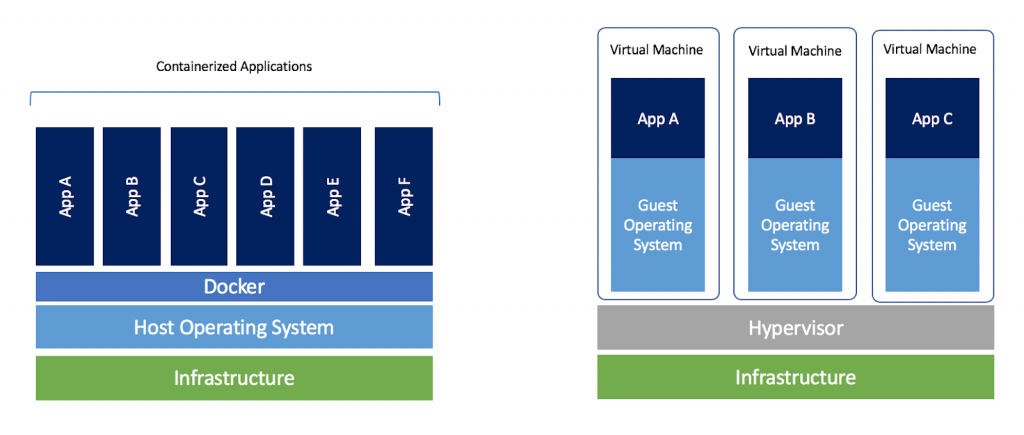
\includegraphics[width=1\textwidth,angle=0]{gfx/vmvsdocker2}
%\caption[Vergleich von Containern und virtuellen Maschinen]{Vergleich von Containern und virtuellen Maschinen % \cite{docker:vmvsdocker}}
%\label{fig:vmvsdocker}
%\end{figure}
%Gemeinsamkeiten finden sich darin, dass beide Technologien eine isolierte Umgebung für das Ausführen von Anwendungen bieten und dass sich sowohl VMs als auch Container aufgrund ihrer Beschaffenheit schnell und ohne Probleme zwischen verschiedenen Hosts umziehen lassen. Auch die Möglichkeit die Ressourcen für die Anwendung zu limitieren wird von beiden Technologien unterstützt.

\section{Kubernetes}
\label{sec:kube}
Kubernetes (griech. für Steuermann) ist eine von Google entworfene Plattform für das automatisierte Verwalten, Skalieren und Bereitstellen von Anwendungen in Containern. Google verwendet schon seit mehr als zehn Jahren Container in seinen Datencentern \cite{Burns2016BorgKubernetes}. Für die Verwaltung dieser wurde vorher die eigens entwickelte Plattform Borg und Omega genutzt. Als auch viele andere Entwickler begannen, sich für Linux-Container zu interessieren, wurde Kubernetes entwickelt \cite{Burns2016BorgKubernetes}. \medskip

Seit 2014 ist das System Open-Source und wird aktuell von der \ac{CNCF} gepflegt. Eine aktuelle Umfrage der \ac{CNCF} zeigt, dass Kubernetes zurzeit die führende Plattform ist und seine Konkurrenten wie Docker Swarm überholt hat \cite{kube:survey}. Ein Unterschied gegenüber anderen Lösungen ist, dass Kubernetes neben Docker auch andere Software für Container einsetzen kann, auf die in dieser Arbeit allerdings nicht weiter eingegangen wird.

\subsection{Kubernetes Architektur}
Ein Kubernetes Cluster besteht aus zwei Komponenten, welche sich in einer sogenannten Master-Slave-Architektur befinden. Die Architektur besteht aus einem Master, welcher aus einem oder mehreren Servern bestehen kann, und den von ihm verwalteten Slaves, in Kubernetes Nodes genannt (Abbildung \ref{fig:kubearchitektur}). Die Komponenten des Clusters können dabei sowohl lokal, auf physischen Servern oder virtuellen Maschinen als auch online auf Infrastruktur von Cloud-Computing Anbietern laufen.
\begin{figure}[htb]
\centering
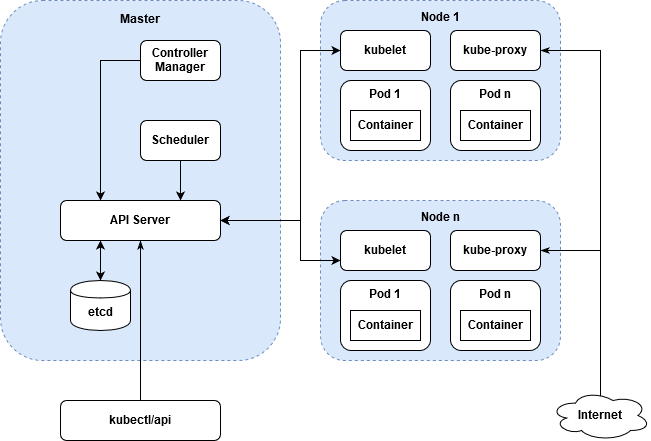
\includegraphics[width=0.8\textwidth,angle=0]{gfx/Kubernetes_Architektur}
\caption[Kubernetes Architektur]{Kubernetes Architektur}
\label{fig:kubearchitektur}
\end{figure}

\subsection{Master Node}
\label{masternode}
Der Master ist verantwortlich für die Verwaltung der Nodes im Cluster. Er leitet die Befehle vom Nutzer an die Nodes weiter. Er enthält mehrere für das Cluster wichtige Komponenten (vergleiche Abbildung \ref{fig:kubearchitektur}). Die Verwendung von mehreren Mastern ermöglicht es, ein hochverfügbares Cluster zu planen \cite[][]{9781788994729}. 

\subsubsection{API}
Der \textit{kube-apiserver} stellt die \ac{API} zur Verfügung, über die jegliche Kommunikation abläuft. Befehle, die der API Server über die Rest-Schnittstelle oder das \ac{CLI} erhält, verarbeitet er und reicht sie weiter \cite{Rensin2015Kubernetes43826}. Über die API ist es möglich, Kubernetes Objekte zu erstellen, zu bearbeiten und zu löschen.

\subsubsection{Controller Manager}
Auf dem \textit{kube-controller-manager} laufen die Controller. Auch wenn jeder Controller ein eigener Prozess sein könnte, werden sie, um die Komplexität zu reduzieren, in einem einzigen Prozess ausgeführt \cite{kube:components}. Dieser läuft auf dem Master und überwacht den Status des Clusters über die API. Verändert sich der gewünschte Status des Clusters, führen sie die nötigen Operationen aus, um das Cluster in den gewollten Status zu versetzen. Ein Beispiel hierfür wäre, wenn die Anzahl der geforderten Replicas nicht der Anzahl der existierenden entspricht. In diesem Fall würden neue Replicas gestartet werden. Der Controller Manager enthält unter anderem folgende Controller:
\begin{description}
\item[Replication Controller]
Der \textit{Replication Controller} ist dafür verantwortlich, die richtige Anzahl an Pods, welche eine logische Gruppe aus einem oder mehreren Containern darstellt (siehe \ref{kube:pod}), für jedes Replication Controller API Objekt beizubehalten.
\item[Endpoint Controller]
Erzeugt Endpoint Objekte, welche für die Verbindung von Services und Pods genutzt werden.
\item[Node Controller]
Bei dem Node Controller handelt es sich um einen Controller, welcher die Verfügbarkeit der Nodes im Clusters überwacht. Er reagiert, sobald ein Node nicht mehr verfügbar ist.
\item[Service Account \& Token Controller]
Dieser Controller er\-zeugt die Standard Accounts und verwaltet die Access Tokens \cite{kube:components}.
\end{description}

\subsubsection{Scheduler}
\label{kube:scheduler}
Um eine gleichmäßige Auslastung der Nodes zu gewährleisten, verteilt der Scheduler die Pods auf die Nodes. Dabei werden verschiedene Faktoren, wie die benötigten Ressourcen für die Anwendung und die Verfügbarkeit von Ressourcen auf dem Node bei der Auswahl der Nodes berücksichtigt. Abhängig vom Zustand des Clusters kann es auch vorkommen, dass Pods von einem Node auf einen anderen verschoben werden \cite{kube:components}.

\subsubsection{etcd}
Etcd\footnote{https://coreos.com/etcd/} ist ein leichtgewichtiger, verteilter Key-Value-Store, der die Konfiguration des Clusters sowie Informationen zu dessen Zustand speichert. Andere Komponenten des Clusters können über REST auf ihn zugreifen \cite[][]{9781788994729}. 

\subsubsection{Add-ons}
Bei Add-ons handelt es sich um Pods oder Services, welche die Funktionalität von Kubernetes erweitern. Ein Beispiel für ein Add-on ist das Web UI (Dashboard) für das Verwalten des Clusters und der Anwendungen, die dort laufen.
% raft consensus algortihm für HA \cite{Ongaro2014InVersion}

\subsection{Worker Node}
\label{workernode}
Sobald eine Anwendung im Cluster gestartet wird, werden die benötigten Pods auf den Nodes verteilt. Die Nodes stellen die Laufzeitumgebung für die Pods zur Verfügung. Jeder Node nutzt dabei dieselben Komponenten \cite{kube:components}. Die zwei wichtigsten Komponenten sind der Kube-Proxy und der kubelet \cite[][]{9781788994729}. 

\subsubsection{kubelet}
Der kubelet verwaltet die Pods und Container auf den Nodes. Er antwortet auf die Befehle vom Master und setzt diese um. Typische Befehle sind zum Beispiel das Erstellen, Überwachen und Zerstören von Containern auf dem Node \cite{Rensin2015Kubernetes43826}.
Eine weitere Aufgabe ist, den Status der Nodes an den Master zu melden.
% abgleich über endpoint/file path oder podscpec (yaml-&gt; updates

\subsubsection{Kube-Proxy}
Beim Kube-Proxy handelt es sich um einen Netzwerk Proxy, der Container und Service (siehe \ref{kube:service}) verbindet. Zusätzlich bietet er eine Lastverteilung. Der Proxy selbst unterstützt kein http, aber beherrscht dafür TCP und UDP Weiterleitung oder Round Robin für eine Lastverteilung.

\subsection{Pod}
\label{kube:pod}
Ein Pod ist die kleinste ausführbare Einheit in einem Kubernetes Cluster und repräsentiert eine laufende Anwendung. Innerhalb eines Pods ist es möglich, einen oder mehrere Container zu starten, welche miteinander gekoppelt sind. Diese teilen sich die Ressourcen wie Speicher, die IP-Adresse im Cluster oder das Netzwerk. Daher ist es Containern in einem Pod möglich, über \textit{localhost}\footnote{\label{foot:localhost}Standardisierter Domainname des aktuellen Computers} miteinander zu kommunizieren. Container in einem Pod werden beim Ausführen nicht über mehrere Nodes verteilt, sondern immer als eine Einheit auf einem Node ausgeführt. Der Node wird dabei durch den \textit{Scheduler} (siehe \ref{kube:scheduler}) anhand der Auslastung der Nodes und der vom Pods angeforderten Ressourcen gewählt.  \medskip

Wird eine Anwendung horizontal skaliert\footnote{\label{foot:scaleout}Erweitern der Kapazität durch zusätzliche Hard- oder Software}, startet ein zusätzlicher Pod, welcher eine eigenständige Instanz darstellt. Kubernetes empfiehlt, keine Pod Objekte von Hand zu erzeugen, und stattdessen ein Deployment (siehe \ref{kube:deployment}) oder für zustandsbehaftete Anwendungen ein StatefulSet (siehe \ref{kube:statefulset}) einzusetzen \cite{kube:pod2}. Ein manuell erzeugter Pod ist im Gegensatz zu von Controllern erzeugten und verwaltenden Pods nicht auf Beständigkeit ausgelegt und würde einen Absturz oder Fehler eines Nodes nicht überstehen.

\subsection{Services}
\label{kube:service}
Ein Service sorgt dafür, dass Pods für den Nutzer erreichbar sind. Ein Service ist ein REST API Objekt und bekommt eine IP-Adresse zugeteilt. Auch jeder Pod im Cluster hat seine eigene IP-Adresse, doch kann es passieren, dass sich ein Pod zum Beispiel durch den Replica Controller ändert. Dadurch würde der Pod eine neue Adresse zugeteilt bekommen. Um dies übersichtlicher zu gestalten und für den Nutzer zu vereinfachen, fügen Services eine zusätzliche Abstraktionsebene hinzu. Ein Service beschreibt dabei eine Regel, wie ein Pod erreicht werden kann. \medskip

Auf welche Pods ein Service weiterleitet, wird meistens über einen Label Selector festgelegt. Ein Label ist ein Key-Value Paar, welches einem Kubernetes Objekt wie einem Pod zugeordnet wird und selbst festgelegt werden kann. Über das Label ist so eine Identifikation des Objektes möglich.

\lstset{language=yaml}
\begin{lstlisting}[frame=hlrtb, caption={Beispiel: Kubernetes Service} ,backgroundcolor=\color{white}, label={lst:kubeservice}]
kind: Service
apiVersion: v1
metadata:
  name: app-service
spec:
  selector:
    app: App
  ports:
  - protocol: TCP
    port: 80
    targetPort: 8080
\end{lstlisting}
In dem Beispiel in Listing \ref{lst:kubeservice} wird ein Kubernetes Service Objekt erzeugt, welches den Namen \textit{app-service} hat. Der Service hat als Ziel Port 8080 bei jedem Pod mit dem Label \textit{App}. Das Ergebnis der Suche nach Pods mit dem festgelegten Label wird in ein Endpoint Objekt gespeichert. Zusätzlich bekommt der Service auch noch eine IP-Adresse im Cluster. Neben Services, welche als Proxy oder Loadbalancer agieren, gibt es in Kubernetes auch noch \textit{Headless Services}. Diese bieten die Möglichkeit, einen Pod direkt anzusprechen, und werden zum Beispiel für ein StatefulSet zwingend benötigt (siehe \ref{kube:statefulset}).
% clusterIP: None # erwähnen?

\subsection{Namespace}
Ein Namespace kann dafür genutzt werden, um verschiedene Bereiche auf dem Cluster, für verschiedene Projekte oder Teams abzugrenzen. Zur Identifizierung erhält der Namespace einen eindeutigen Namen. Durch Namespaces ist es ebenfalls möglich, Ressourcen zu limitieren.

\subsection{Ingresses}
Mit einem Ingress bietet Kubernetes eine einfache Möglichkeit, Zugriff auf Ressourcen des Clusters von außerhalb zu gewähren. Ein Kubernetes Cluster ist ein eigenes Netzwerk und isoliert grundsätzlich vor dem Zugriff von außen. In dem Ingress Objekt werden Regeln für das Routing über \ac{HTTP} oder \ac{HTTPS} von außerhalb sowie für die Konfiguration des Ingress gespeichert. Zusätzlich bietet er Optionen für Lastverteilung und SSL Termination. \medskip

Für den Ingress kann verschiedene Software benutzt werden. Im Kubernetes Projekt wird ein Nginx\footnote{\label{foot:nginx}Ein Open-Source Webserver, der auch als Reverse-Proxy genutzt werden kann} Ingress Controller und ein \ac{GCE} Ingress Controller unterstützt und gewartet.
%

\subsection{Controller}
Die unterschiedlichen Controller bieten für das Verwalten der Pods verschiedene Funktionen, die sich für verschiedene Einsatzzwecke eignen. Ein Controller läuft dabei in einer Kontrollschleife, welche den Zustand der von ihm verwalteten Pods über die Kubernetes API überwacht. Sollte der gewünschte Zustand vom aktuellen abweichen, führt er die nötigen Schritte aus, um den Zustand zu ändern.

\subsubsection{ReplicaSet \& ReplicationController}
Ein ReplicationController oder ReplicaSet sorgt dafür, dass mehrere Instanzen eines Pods existieren. Falls die Anzahl der angeforderten Replicas sich ändern sollte, sorgt der Controller dafür, dass weitere Replicas erzeugt oder entfernt werden. Durch diese Funktion lassen sich große Lasten verarbeiten oder eine höhere Verfügbarkeit erreichen. Eine Replica ist dabei eine Kopie eines Pods. Um die Anzahl der Replicas oder die Pods zu konfigurieren, wird ein sogenanntes Pod Template verwendet \cite{Rensin2015Kubernetes43826}. Trotz des Namens ist dieser Controller auch für einzelne Pods ohne Replicas sinnvoll, da er die Anzahl der Pods überwacht und so auf mögliche Abstürze reagiert.
Der bisher einzige Unterschied zwischen einem ReplicationController und dem neueren ReplicaSet ist die Art, wie sie Pods auswählen. Wird ein Controller entfernt bleiben die von ihm verwalteten Pods enthalten.
% Während der ReplicationController einen \textit{Equality Based Selector} verwendet, nutzt das ReplicaSet einen \textit{Set-Based Selector}.

\subsubsection{Deployment}
\label{kube:deployment}
Ein Deployment ist ein, in 2016 mit der Kubernetes Version 1.2 veröffentlichter Controller, der die Funktionalität eines ReplicaSets erweitert \cite[][]{9781788994729}. Für Pods die im Pod Template beschrieben sind, wird ein ReplicaSet erzeugt. Durch die zusätzliche Abstraktionsebene setzt er einige Funktionen wie zum Beispiel \textit{Rolling Updates} um. Dabei wird ein zusätzliches ReplicaSet für die neue Version des Pods gestartet und die alte erst entfernt, wenn die neue einwandfrei läuft. Kommt es zu Fehlern, wird das Update nicht ausgeführt.
Das Pod Template beschreibt, wie auch bei den anderen Controllern, einen gewünschten Zustand, den das Deployment überwacht und herstellt. Sollte ein Pod unerwartet abstürzen, wird er auch hier neu gestartet. \medskip

Das Listing \ref{lst:kubedeployment} zeigt beispielhaft eine YAML-Datei, welche dafür genutzt wird, ein Deployment Objekt, welches einen Postgres Datenbank Pod enthält, zu erzeugen.  \medskip
\newpage

\lstset{language=yaml}
\begin{lstlisting}[frame=hlrtb, caption={Beispiel: Kubernetes Deployment} ,backgroundcolor=\color{white}, label={lst:kubedeployment}]
apiVersion: apps/v1
kind: Deployment
metadata:
  name: postgres-deployment
spec:
  selector:
    matchLabels:
    app: postgres
  replicas: 2
  template:
    metadata:
      labels:
        app: postgres
    spec:
      containers:
      - name: postgres
        image: postgres:9.6
        ports:
        - containerPort: 5432
\end{lstlisting}
%empohlener Kontroller, RelicaSet nur wenn Updates selber machen will oder garkeine Braucht.

\subsubsection{StatefulSet}
\label{kube:statefulset}
Das \textit{StatefulSet} eignet sich besonders für Anwendungen, deren Zustand bewahrt werden soll. Im Gegensatz zu einem Deployment sorgt es dafür, dass Pods eine einzigartige Bezeichnung bekommen, welche über die Laufzeit hinweg bestehen bleibt. Anhand dieser Bezeichnungen werden dem StatefulSet auch die Ressourcen zugeteilt. Wird ein Pod mit denselben Spezifikationen erneut gestartet, bekommt er vom Controller dieselbe Bezeichnung und die gleichen Ressourcen zugeteilt. Darüber hinaus bieten StatefulSets die Möglichkeit, Pods geordnet zu starten.
Auch der StatefulSet Controller, welcher seit Version 1.9 in einer stabilen Version verfügbar ist, versucht, wie die anderen Controller, einen gewünschten Zustand herzustellen. Sollte der Zustand nicht der gewünschte sein, werden die nötigen Schritte, um ihn zu ändern, eingeleitet. Zusätzlich benötigt ein \textit{StatefulSet}, im Gegensatz zu einem ReplicaSet oder einem Deployment, noch einen \textit{Headless Service} (siehe \ref{kube:service}) für die Identifizierung im Netzwerk.
Das Entfernen eines StatefulSet löscht nicht die mit den Pods verbunden Ressourcen. So kann für zustandsbehaftete Anwendungen die Datensicherheit garantiert werden.

\subsubsection{DaemonSet}
Der Daemonset Controller sorgt dafür, dass auf jedem Node oder einem Teil der Nodes des Clusters eine Instanz eines Pods läuft. Daher eignet sich dieser Controller besonders gut für Daemons oder Agents. Sollte ein Node vom Cluster entfernt oder zum Cluster hinzugefügt werden, kümmert sich der Controller darum, die Anzahl der Instanzen an die Anzahl der Nodes anzupassen.

\subsection{Helm}
Helm ist ein Werkzeug zum Verwalten von Anwendungen in Kubernetes. In sogenannten Helm Charts wird der Zustand von Anwendungen definiert. Die Verwendung von Helm vereinfacht sowohl die Installation als auch die Wartung der Anwendungen. Dabei ist es möglich, Objekte dynamisch zu definieren, oder Werte, ohne direktes Bearbeiten der Dateien, zu überschreiben. Dadurch ist es zum Beispiel ohne Aufwand möglich, eine andere Version eines Docker Images einzubinden. Wie auch Kubernetes wird Helm von der \ac{CNCF} verwaltet \cite{Helm}. Helm bietet einen offiziellen Katalog, der Anwendungen in stabilen Charts zur Verfügung stellt und standardmäßig installiert wird \cite{helm:github}. Diese können durch den \textit{helm install} Befehl installiert werden.

\subsubsection{Helm Charts}
\label{helm:chart}
Die sogenannten Helm Charts bestehen aus einem Verbund mehrerer Dateien, welche die Anwendung und ihren Zustand definieren. Dabei werden verschiedene Charts über die Verzeichnisstruktur abgegrenzt. Wichtige Dateien sind die \textit{Charts.yaml}, welche allgemeine Informationen über den Chart enthält, die \textit {requirements.yaml}, welche Informationen über Abhängigkeiten enthält und die \textit{values.yaml}, welche für die Konfiguration der den Variablen zugeordneten Werten genutzt wird.

\section{Persistenz in Kubernetes}
Für die persistente Speicherung von Daten kann in Kubernetes zwischen einer Vielzahl an Möglichkeiten gewählt werden. Durch die Verwendung von Volume Plugins ist es möglich, Volumes dynamisch erzeugen zu lassen oder sie bereits vorher für die Verwendung zu erzeugen. \medskip
\begin{figure}[htb]
\centering
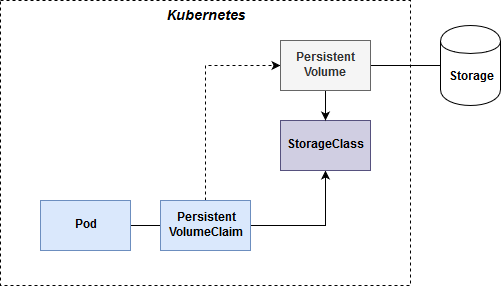
\includegraphics[width=0.8\textwidth,angle=0]{gfx/kubevolumelifecycle}
\caption{Zusammenhang Pod und Volume}
\label{fig:kubevolumelifecycle}
\end{figure}


Die Konfiguration des von Pods angeforderten Speichers geschieht direkt bei der Konfiguration des Pods über ein sogenanntes \ac{PVC}. Bei der statischen Bereitstellung von Volumes wird zunächst geprüft, ob ein \ac{PV} mit mindestens der geforderten Größe existiert, und das am besten passende eingebunden. Wird hier kein \ac{PV} gefunden und ist die dynamische Erstellung nicht konfiguriert, wird auf die Erzeugung eines Speichers gewartet \cite{kube:pv}. Die dynamische Methode bietet die Möglichkeit, das benötigte Volume durch das in der \ac{SC} Provisioner genannte Volume Plugin erzeugen zu lassen. \medskip

Die Abbildung \ref{fig:kubevolumelifecycle} zeigt den Ablauf der Erstellung eines \ac{PV}s. Fordert ein Pod durch eine \ac{PVC} Speicher an, so erstellt die \ac{SC} dynamisch ein \ac{PV}, welches der Konfiguration des \ac{PVC} entspricht.

\subsection{Persistent Volumes}
\label{kube:pv}
Ein PersistentVolume bietet in Kubernetes die Möglichkeit, Daten persistent zu speichern. So sind Daten erneut verfügbar sollte ein Pod aufgrund eines Fehlers neu gestartet werden. Die Verwendung von \ac{PV}s ermöglicht es, die Art und Weise wie der Speicher genutzt wird von der Bereitstellung abstrahiert zu betrachten. Für die Bereitstellung von \ac{PV}s gibt es zwei Möglichkeiten. Bei der statischen Provisionierung ist es nötig, dass alle \ac{PV}s manuell angelegt werden. Direkt nach dem Anlegen sind sie für die Nutzung verfügbar. Die zweite Möglichkeit ist das dynamische Provisionieren. Dabei wird ein neues Volume für die Anforderungen erzeugt. Dafür wird das \ac{PVC} des Pods betrachtet, in dem der angeforderte Speicher konfiguriert ist. Dort ist neben der Größe des Speichers und weiteren Einstellungen auch eine \ac{SC} definiert \cite[][]{9781788994729}. 

\subsection{Persistent Volume Claim}
\label{kube:pvc}
Durch ein \ac{PVC} ist es möglich, das gewünschte \ac{PV} näher zu spezifizieren. Es lässt sich bereits während der Erstellung des Pods konfigurieren. Dabei enthält ein \ac{PVC} Objekt einige Informationen wie einen Namen für die Identifikation, die Größe des benötigten Speichers und einige weitere Einstellungen für den Speicher (Listing \ref{lst:kubepvc}).  \medskip

Der Zugriffsmodus ist eine wichtige Einstellung, welche definiert, wie der Speicher eingebunden ist. Der Speicher kann nach Bedarf nur mit Leserechten oder mehrfach eingebunden werden. Dadurch lässt sich der Speicher unterschiedlichen Einsatzzwecken anpassen.
\begin{description}
\item[ReadWriteMany]
\ac{RWX} erlaubt es, den Speicher in einem oder mehreren Pods einzubinden. Dadurch ist es möglich, dass Pods über den Speicher Daten austauschen. Schreib- sowie Lesezugriff sind möglich.
\item[ReadWriteOnce]
\ac{RWO} erlaubt es, einen Speicher in genau einem Pod einzubinden. Schreib- sowie Lesezugriff sind möglich.
\item[ReadOnlyMany]
\ac{ROX} kann wie \ac{RWX} mehrfach eingebunden werden, allerdings sind nur Lesezugriffe möglich. Daher eignet es sich vorallem für statische Daten, die in mehreren Pods verfügbar sein sollen.
\end{description}
Die nächste wichtige Option ist die Wahl der \ac{SC}. Sie wird für die dynamische Erstellung von Speicher benötigt (siehe \ref{kube:sc}).
\lstset{language=yaml}
\begin{lstlisting}[frame=hlrtb, caption={Beispiel: Kubernetes PersistentVolumeClaim (PVC)} ,backgroundcolor=\color{white}, label={lst:kubepvc}]
kind: PersistentVolumeClaim
apiVersion: v1
metadata:
  name: claim
spec:
  accessModes:
  - ReadWriteOnce
  resources:
    requests:
      storage: 8Gi
  storageClassName: sc-name
\end{lstlisting}
Das Listing \ref{lst:kubepvc} zeigt eine beispielhafte Konfiguration eines \ac{PVC}. Dabei wird von der \ac{SC} \textit{sc-name} ein Speicher mit einer Kapazität von acht GB und dem Zugriffmodus \ac{RWO} angefordert.

\subsection{Storage Class}
\label{kube:sc}
Durch die Verwendung von mehreren \ac{SC}s ist es möglich, verschiedene Arten von Speicher anzubieten. So kann durch den Einsatz unterschiedlicher Technologien oder der Einbindung von unterschiedlicher Hardware auf unterschiedliche Anforderungen reagiert werden. \medskip

Es ist möglich, eine \ac{SC} als Standard zu benennen, welche immer wenn in einem \ac{PVC} keine \ac{SC} benannt wird genutzt wird.
Das \ac{SC} Objekt enthält Informationen wie das als Provisioner gewählte Volume-Plugin und Parameter, um ihn zu konfigurieren. Desweiteren lassen sich Regeln für eine erneute Beanspruchung von dynamisch erstellten Volumen oder zusätzliche Optionen für das Einbinden des Speichers konfigurieren. Mögliche Regeln für die erneute Beanspruchung sind Retain, Delete und Recyle.
\begin{description}
\item[Retain]
Retain bedeutet nach dem Löschen des \ac{PV} bleiben die Daten bestehen und müssen manuell auf dem System gelöscht werden. Durch ein erneutes Erstellen des dazugehörigen \ac{PV} lassen sich die Daten erneut nutzen.
\item[Delete]
Bei Delete werden durch das Löschen des dazugehörigen \ac{PV} die Daten auf dem System automatisch entfernt. Bei dynamisch erstellten \ac{PV}s werden die Regeln für eine erneute Beanspruchung der StorageClass verwendet. Falls in der StorageClass keine Regeln spezifiziert wurden, ist \textit{Delete} der Standardwert.
\item[Recycle]
Recycle ist eine veraltete Regel, welche durch das dynamische Provisionieren ersetzt wurde. Sie entfernt den Inhalt des eingebundenen \ac{PV}s. Dadurch ist es bereit, erneut eingebunden zu werden.
\end{description}
\lstset{language=yaml}
\begin{lstlisting}[frame=hlrtb, caption={Beispiel: Kubernetes StorageClass}
,backgroundcolor=\color{white}, label={lst:kubesc}]
kind: StorageClass
apiVersion: storage.k8s.io/v1
metadata:
  name: standard
provisioner: kubernetes.io/provisioner
reclaimPolicy: Retain
volumeBindingMode: Immediate
\end{lstlisting}
Das Listing \ref{lst:kubesc} zeigt beispielhaft die Erstellung einer \ac{SC} mit dem Namen \textit{standard}. Neben der Wahl des Provisioners \textit{kubernetes.io/provisioner} wird die Regel für die erneute Beanspruchung des Speichers auf \textit{Retain} gesetzt.

\subsection{Volume Plugin System}
Ohne Hilfe durch Tools müssten von Dritten erstellte Plugins fest in Kubernetes integriert und mit Kubernetes ausgeliefert werden. Um auch ohne diese Integration die Möglichkeit zu haben eigene Volume Plugins erstellen zu können, existieren derzeit zwei Möglichkeiten. Das seit Version 1.2 existierende Flex Volume, welches eine \ac{API} für externe Plugins bereitstellt, oder das seit Version 1.10 im Beta Status existierende \ac{CSI}.

\subsubsection{FlexVolume}
Bei FlexVolume handelt es sich um ein Tool, welches eine API für Volume Plugin von Dritten zur Verfügung stellt. Um die Speichertreiber zu nutzen, müssen die Nodes vorbereitet werden und die nötigen Daten auf das System kopiert werden. Dafür wird Zugriff auf alle Nodes des Clusters benötigt. Seit Version 1.8 erkennt FlexVolume, ohne einen Neustart der betroffenen Nodes, wenn neue Treiber hinzugefügt oder alte aktualisiert werden.

\subsubsection{Container Storage Interface}
Das \ac{CSI} ist eine Schnittstelle für Plattformen wie Kubernetes, um die Persistenzlösungen den Containern zugänglich zu machen. Es befand sich bis Version 1.12 im Beta Status und ist seit der Version 1.13 in einer stabilen Version verfügbar. \medskip

Eine Konfiguration des \ac{CSI} ist über Parameter möglich. Dort lassen sich der Treiber, der genutzt werden soll, die Art des Dateisystems und weitere Optionen konfigurieren.

\chapter{Anforderungsanalyse}
\label{cha:anfoderungen}
Dieses Kapitel der Thesis untersucht die Anforderungen an die persistente Speicherung von Daten. Dafür wird zunächst das Projekt betrachtet und die zu erwartenden Anwendungsfälle analysiert. Anschließend werden darauf aufbauend die Anforderungen für die Persistenzlösung formuliert.

\section{Das Projekt}
\label{projekt}
Die Idee der ALM v2.0 ist eine \ac{ALM} Umgebung für die automatisierte Installation und Konfiguration eines Atlassian Stacks durch eine Container Orchestration Lösung. Ziel ist, den Prozess der Bereitstellung, welcher vorher mehrere Tage in Anspruch genommen hat, auf eine möglich kurze Zeit zu reduzieren. Der Atlassian Stack ist eine Tool-Sammlung des Softwareherstellers Atlassian, welche den Prozess der Produkt- und Softwareentwicklung begleitet. \medskip

Um dieses Ziel umzusetzen, wurden die Prozesse der Installation und Konfiguration automatisiert und die grundlegende Infrastruktur verändert. Während zuvor für jede Anwendung eine einzelne virtuelle Maschine erstellt wurde, werden in der prototypischen Umsetzung der ALM v2.0 die containerisierten Anwendungen gestartet. Dafür wurden zunächst Container erstellt, die über ein Dockerfile (siehe \ref{subsec:dockerfile}) die Anwendungen installieren und für den ersten Start konfigurieren. Basierend auf diesen Containern wurden anschließend Helm Charts (siehe \ref{helm:chart}) entworfen, welche neben den Anwendungen selbst noch einen vorgefertigten Datenbank-Container und einen weiteren Container für die Erstkonfiguration der Anwendung durch ein in Python entworfenes Script enthalten. \medskip

Um den Zustand der ausgeführten Anwendungen zu bewahren, werden die Anwendung und die Datenbank als StatefulSet gestartet (siehe \ref{kube:statefulset}). Neben einer eindeutigen Identifizierung der Anwendung ermöglicht dies die erneute Zuteilung des dynamisch erstellten Datenträgers. Um die Helm Charts anschließend auszuführen, steht ein Kubernetes Cluster bereit, welches verteilt auf mehreren virtuellen Maschinen läuft. Für die persistente Speicherung der Daten wird zurzeit ein ebenfalls auf einer virtuellen Maschine laufender einzelner \ac{NFS} Server genutzt.
 
\section{Anwendungsfälle}
Bevor Anforderungen für das Projekt aufgestellt werden, muss betrachtet werden, in welchen Situationen die Lösung eingesetzt wird. Dies geschieht, indem die zu erwarteten Anwendungsfälle betrachtet werden. Für die Auswahl einer Lösung für die persistente Speicherung von Daten in einem Cluster werden dabei nicht nur Situationen während des Betriebs von Anwendungen sondern auch die Installation und die Wartung betrachtet. Aus den beispielhaften Szenarien werden anschließend die Anforderungen extrahiert.

\subsection{Auswahl, Installation und Betrieb der Speicherlösung}
Für die ausgewählte Persistenzlösung steht bestehende Infrastruktur bereit. Da auf der Infrastruktur sowohl das Kubernetes Cluster als auch verschiedene andere Anwendungen betrieben werden, ist zu überprüfen, welche Ressourcen zur Verfügung stehen, und mit dem Bedarf abzugleichen. Um auf mögliche Veränderungen der Infrastruktur oder der Auslastung des Clusters zu reagieren, soll die Lösung skalierbar sein.

\subsection{Ausführen von Stateful Anwendungen}
Die Hauptaufgabe des Kubernetes Clusters ist das Ausführen von Anwendungen. Dabei handelt es sich aktuell größtenteils um Stateful Anwendungen. Im späteren Verlauf des Projekts sollen einige Anwendungen selbst in einem Cluster ausgeführt werden, um neue Funktionen wie das Zero-Downtime Upgrade zu nutzen. Dafür muss, um die Daten der Anwendungen synchron zu halten, zusätzlich in jeder Instanz der Anwendung der gleiche Speicher eingebunden werden. Neben den Anwendungen selbst wird darüber hinaus oft noch eine Datenbank benötigt. Beide Pods benötigen das persistente Speichern ihrer Daten, um einen stabilen Betrieb zu gewährleisten. Um die Chance auf Ausfälle gering zu halten, soll die Software bereits in einer stabilen Version vorliegen.

\subsection{Veränderung von Dateien auf dem Dateisystem der Pods}
Neben dem Betrieb der Anwendungen selbst, ist vor allem die Konfiguration dieser wichtig. Einige Einstellungen lassen sich nur durch das Verändern der Daten auf Dateisystemebene der Anwendung konfigurieren. Ein Nutzer, der administrativen Zugriff auf die Anwendung hat, soll, ohne administrativen Zugriff auf das Kubernetes Cluster zu benötigen, die Daten anpassen können.

\subsection{Sicherheit der Daten}
Die persistent gespeicherten Daten sollen auch bei Ausfällen oder Fehlern im System erhalten bleiben. Unabhängig davon durch welche Funktionen oder Technologien dieses Problem gelöst wird, muss die Reaktion des Systems zuverlässig sein.

\section{Anforderungen}
Aufbauend auf den beispielhaften Anwendungsfällen lassen sich die Anforderungen ableiten. Diese werden näher beschrieben und in zwei Kategorien eingeteilt.

\subsection{Funktionale Anforderungen} % (fold)
\label{sec:funktionale}
Funktionale Anforderungen sind Anforderungen, welche Funktionen oder Dienste der Persistenzlösung näher spezifizieren. Um die Anzahl an möglichen Speicherlösungen einzugrenzen, werden sie zu Beginn anhand der funktionalen Anforderungen verglichen.

\subsubsection{Mehrfachzugriff auf den eingebundenen Speicher}
Um dem Nutzer die Möglichkeit zu geben, die Anwendung ohne administrativen Zugriff auf das Cluster selbst zu konfigurieren, ist es nötig, ihm Zugriff zum Speicher zu gewähren. Dabei soll es sich um eine Schnittstelle handeln, auf die ohne großen Aufwand zugegriffen werden können. Eine Option wäre es, Speicher zu verwenden, die mehrfach eingebunden werden können. Dies hätte ebenfalls zur Folge, dass die Speicherlösung im späteren Verlauf des Projekts, wenn die Anwendungen im Cluster ausgeführt werden, verwendet werden kann. Die Persistenzlösung soll daher eine Lösung sein, welche mehrfache Schreib- und Lesezugriffe unterstützt, also den Zugriffsmodus \ac{RWX} unterstützt (siehe \ref{kube:pvc}).

\subsubsection{On-Premises}
Eine weitere Anforderung ist das Verwenden der bestehenden Systeme. Die Software soll daher On-Premise, also lokal, im internen Netzwerk betrieben werden. Auch wenn zurzeit eine Verbindung zum Internet besteht, soll sie auch ohne diese funktional sein.

\subsection{Nichtfunktionale Anforderungen} % (fold)
\label{sec:nichtfunktionale}
Neben den funktionalen Anforderungen, welche sich oft aus einer Funktion oder einem Dienst ableiten, gibt es die nichtfunktionalen Anforderungen. Diese enthalten zusätzliche Voraussetzungen wie Qualitätsmerkmale oder Einschränkungen.

\subsubsection{Ausfallsicherheit}
Um einen fehlerfreien Betrieb zu gewährleisten, sollte die Software eine hohe Verfügbarkeit aufweisen. Durch eine hochverfügbare Architektur und das Verwenden von Redundanzen kann auf Ausfälle von einzelnen Festplatten oder ganzen Servern reagiert werden. Dabei ist darauf zu achten, dass die Redundanzen auf möglichst vielen verschiedenen Servern platziert werden, um einen \ac{SPoF} zu vermeiden. \medskip

Die Ausfallsicherheit gilt als erfüllt, wenn die Software sowohl automatisch Redundanzen erzeugt als auch eine hochverfügbare Architektur aufweist oder andere technische Vorkehrungen für eine hohe Verfügbarkeit trifft. 

\subsubsection{Datensicherung}
Für die Evaluation der Persistenzlösung werden hier die technischen Maßnahmen für Sicherungen der Daten betrachtet. Dafür ist zu prüfen, mit welchem Aufwand automatische, regelmäßige Datensicherungen erstellt werden können, sowie um welche Art von Backup es sich handelt. Unterschieden werden kann hier zwischen vollständigen und inkrementellen Backups. Auch der Wiederherstellungsprozess soll einfach ausführbar sein. Neben Sicherungen können Funktionen wie Snapshots für Tests der im Cluster laufenden Anwendungen hilfreich sein, da sie ermöglichen zwischen verschiedenen Ständen der Daten zu wechseln.  \medskip

Die Anforderung gilt daher als erfüllt, wenn die Speicherlösung automatisierte Sicherungen erstellen und wiederherstellen kann. Zusätzlich sollte sie ebenfalls eine Funktion zum Erstellen von Snapshots bieten.

\subsubsection{Datenintegrität}
Die Datenintegrität stellt die Unversehrtheit der Daten dar. Die Software soll automatisiert fehlerhafte Daten erkennen und entweder den Anwender benachrichtigen oder sie korrigieren. Dafür ist zu betrachten, welche Funktionen oder Algorithmen existieren, um korrupte Daten aufzuspüren.

\subsubsection{Skalierbarkeit}
Um auf Änderungen der vom Cluster benötigten Speicherkapazität oder Leistung reagieren zu können, sollte die Lösung skalierbar sein. Die Lösung sollte sich sowohl vertikal, durch das Hinzufügen von Ressourcen zu einem bestehenden Server, als auch horizontal, durch das Hinzufügen von weiteren Servern, erweitern lassen.

\subsubsection{Geringer Ressourcenbedarf}
Die Software soll auf einem bereits bestehenden System eingesetzt werden. Um dabei einen stabilen Betrieb des Kubernetes Clusters sowie auch anderer Anwendungen zu gewährleisten, muss auf den Ressourcenbedarf geachtet werden. \medskip 

Die Speicherlösung soll, unabhängig von der Anzahl der Nodes und der Kapazität der Festplatte, vorerst nicht mehr als vier Gigabyte Arbeitsspeicher und vier Prozessorkerne benötigen.

\subsubsection{Benutzerfreundlichkeit}
Um die Benutzerfreundlichkeit näher zu bewerten, ist zu klären, aus welcher Perspektive diese bewertet wird. Den Nutzern der Anwendungen des Kubernetes Clusters bleibt die Speicherlösung bis auf das Einbinden des Speichers eines Pods, um Dateien über ein Protokoll wie \ac{NFS} zu modifizieren, verborgen. Daher bewertet die Benutzerfreundlichkeit vor allem die Einfachheit der Installation und Wartung während des Betriebs.  \medskip

In der folgenden Evaluation wird vor allem das Vorhandensein einer Dokumentation und von Scripts für eine automatische Installation und Wartung betrachtet. 

\subsubsection{Wartbarkeit}
Neben der Einfachheit der Wartung gibt es vieles, um die Fehleranfälligkeit zu verringern und somit die Wartbarkeit zu verbessern. So bietet eine Persistenzlösung, welche bereits lange am Markt etabliert ist, viele Erfahrungsberichte und oft auch eine gute Dokumentation. Auch kann die Nutzung einer als stabil markierten Version die Fehleranfälligkeit verringern und so für eine seltenere Wartung sorgen. Zusätzlich ist zu betrachten, ob die Lösung Open-Source ist oder von einem Unternehmen entwickelt wird. Ist eine Lösung Open-Source, so kann die Community den Quellcode einsehen und an der Entwicklung oder Korrektur von Fehlern teilhaben. Zusätzlich kann eine Schnittstelle für Monitoring die Fehlersuche erleichtern.

\section{Zusammenfassung der Anforderungen} % (fold)
\label{sec:uebersichtanfoderungen}
In der Tabelle \ref{listeanforderungen} werden die in \ref{sec:funktionale} und \ref{sec:nichtfunktionale} genannten Anforderungen aufgelistet.
Neben einer Nummer für die Identifizierung erhalten die nichtfunktionalen Anforderungen eine weitere Spalte mit technischen Anforderungen. Werden diese erfüllt, gilt die nichtfunktionale Anforderung ebenfalls als erfüllt.

%Aufgrund der, im Vergleich zu den anderen Anforderungen, geringen Priorität, fließt diese Anforderung allerdings nicht direkt in die Bewertung rein und wird vor allem in der Zusammenfassung der Bewertung, sowie in der Handlungsempfehlung erwähnt.
%evtl erweitern um zukunftsicherherug

\begin{table}[htbp]
\centering
\resizebox{\linewidth}{!}{%}
\begin{tabular}{lll}\hline
\textbf{ID} & \textbf{Beschreibung} &  \\ \hline
\multicolumn{3}{l}{Funktionale Anforderungen}\\ \hline
01 & On-Premises Hosting & \\
02 & Mehrfaches Einbinden des Speichers & \\
\\ \hline
\multicolumn{2}{l}{Nichtfunktionale Anforderungen} & Technische Anforderungen\\ \hline
03 & Ausfallsicherheit & \\ \hline
&& Redundanzen\\
&& Hochverfügbarkeit\\ \hline
04 & Datensicherung & \\ \hline
&& Automatische Sicherung\\
&& Fehlerfreie Wiederherstellung \\
&& Snapshots \\ \hline
05 & Datenintegrität & \\ \hline
&& Fehlererkennung\\
&& Fehlerkorrektur\\ \hline
06 & Skalierbarkeit & \\ \hline
&& Vertikale Skalierbarkeit \\
&& Horizontale Skalierbarkeit \\ \hline
07 & Geringer Ressourcenbedarf & \\ \hline
&& Ressourcenbedarf maximal\\
&& vier Cores und vier GB Arbeitsspeicher \\ \hline
08 & Benutzerfreundlichkeit&  \\ \hline
&& Automatisierte Installation\\
&& Automatisierte Wartung \\ \hline
09 & Wartbarkeit &  \\ \hline
&& Stabile Version\\
&& Etablierte Software \\
&& Dokumentation \\
&& Open-Source \\
\end{tabular}}
\caption{Liste der Anforderungen}
\label{listeanforderungen}
\end{table}


% Kosten?
% Zukunftsicherheit
% evtl - o + 
% negativ = nicht vorhanden, o durch zusätzliche Software und + bereits intergriert.
% Bewertung erklären oder bei evaluation
%evtl erweitern um zukunftsicherherug
%@Wartbarkeit
%Opensoucrce, Öffentlich Dokumentation
%	Vorerst verzicht auf bezahlten Support
%Stabile Vertsion? % 
%Kosten?
% Zukunftsicherheit
% evtl - o + 
% Split brain?
% negativ = nicht vorhanden, o durch zusätzliche Software und + bereits intergriert.
% Bewertung erklären oder bei evaluation

\chapter{Evaluation}
\label{cha:evaluation}

Dieser Abschnitt widmet sich der Evaluation der in Kubernetes existierenden Persistenzlösungen. Dafür werden zuerst die in der Kubernetes Dokumentation genannten Volume Plugins näher betrachtet. Die Lösungen, welche die funktionalen Anforderungen aus \ref{sec:funktionale} erfüllen, werden anschließend analysiert und danach anhand der in \ref{sec:nichtfunktionale} genannten nicht-funktionalen Anforderungen bewertet. Abschließend wird eine Handlungsempfehlung basierend auf den Ergebnissen der Evaluation formuliert.

\section{Marktübersicht}
Die Tabelle \ref{marktuebersicht} im Anhang zeigt die in der Kubernetes Dokumentation genannten Persistenzlösungen \cite{kube:volumes}. Für Lösungen, welche die \ac{CSI} oder Flexvolume Schnittstelle nutzen, wurde universal ein entsprechender Eintrag erstellt. Zusätzlich zu den Namen der Volume Plugins wurden Spalten für die funktionalen Anforderungen, also die Zugriffmodi und das On-Premise Hosting, erstellt. Dadurch ist bereits hier eine Eingrenzung möglich.

% Mehr auf Tabelle im Ahang eingehen und weg zur zweiten Tabelle erklären
% Kein CSI / FLexvolume da keine spezifische Lösung sondern platzhalter

\begin{table}[h!]
\centering
\begin{tabular}{lcccc} \hline
\textbf{Volume Plugin} & \textbf{On-Premises} & \textbf{RWO} & \textbf{ROX} & \textbf{RWX}\\ \hline
CephFS & x & x & x & x\\
CSI & \multicolumn{4}{c}{Abhängig von Treiber} \\
Flexvolume & \multicolumn{4}{c}{Abhängig von Treiber} \\
GlusterFS & x & x & x& x\\
Quobyte & x & x & x& x\\
NFS & x & x & x& x\\
PortworxVolume & x & x & & x \\

\end{tabular}
\caption{Persistenzlösungen, welche die funktionalen Anforderungen erfüllen}
\label{marktuebersicht2}
\end{table}
Die Tabelle \ref{marktuebersicht2} zeigt die Lösungen, welche die funktionalen Anforderungen bereits erfüllen, und sich so für das existierende System eignen. Sowohl \ac{CSI} als Flexvolume bieten durch das Einbinden einer eigens oder von Dritten entwickelten Lösung, die Möglichkeit, die Anforderungen zu erfüllen. Da es sich dabei allerdings um keine spezifische Speicherlösung handelt, werden diese in der Evaluation nicht näher betrachtet. 

\subsection{NFS}
Das \ac{NFS} ist ein UNIX-Protokoll, welches den Zugriff auf Dateien über das Netzwerk ermöglicht. Dabei kann der Server Teile seines eigenen Dateisystems freigeben. Auf Clientseite wird ein Pfad über einen Befehl eingebunden. Anschließend kann auf die im eingebundenen Verzeichnis existierenden Ordner und Dateien zugegriffen werden, als wären sie eine lokal existierende Festplatte. Da es sich um ein Protokoll handelt, können die Daten von unterschiedlichen Programmen zur Verfügung gestellt werden, welche unterschiedliche Features ermöglichen.
% Client Server, Speichern an zentralen Ort

\subsubsection{Einbinden in Kubernetes}
\label{eva:nfskube}
Um einen bereits existierenden NFS Server in Kubernetes einzubinden und ihn für die dynamische Erstellung von Speicher zu Nutzen, wird neben einer \ac{SC} die Anwendung \textit{nfs-client-provisioner} benötigt. Dieser kann unter Hilfe von einem gleichnamigen Helm Chart installiert werden.
\lstset{language=bash}
\begin{lstlisting}[frame=hlrtb, caption={nfs-client-provisioner: Installation} ,backgroundcolor=\color{white}, label={lst:nfs}]
$ helm install stable/nfs-client-provisioner --set nfs.server=172.168.10.100 --set nfs.path=/data/kubernetes
\end{lstlisting}
Für die Installation ist nur ein Kommando notwendig (Listing \ref{lst:nfs}). Über dieses Kommando werden zusätzliche Parameter wie die Netzwerkadresse des Servers, der Pfad der eingebunden werden soll und auch der Name der erstellten StorageClass (Listing \ref{lst:nfssc}) definiert.
\lstset{language=yaml}
\begin{lstlisting}[frame=hlrtb, caption={StorageClass nfs-client-provisioner} ,backgroundcolor=\color{white}, label={lst:nfssc}]
apiVersion: storage.k8s.io/v1
kind: StorageClass
metadata:
  name: nfs-sc
provisioner: nfs-client-provisioner
parameters:
  archiveOnDelete: "false"
\end{lstlisting}

\subsection{GlusterFS}
\label{subsec:gluster}
Bei GlusterFS handelt es sich um eine Open-Source Persistenzlösung, welche ein skalierbares und verteiltes Dateisystem erzeugt, das es ermöglicht, Speicher von mehreren Servern als virtuelles Laufwerk zur Verfügung zu stellen \cite{Bertsche2018ClusterPostgreSQL}. Um ein vorhandenes System zu skalieren, kann die Speicherkapazität der einzelnen Nodes erweitert oder neue Nodes in das Cluster hinzugefügt werden. Im Gegensatz zu anderen Lösungen nutzt Gluster weder einen zentralen, noch einen verteilten Server für die Metadaten, sondern setzt den \ac{EHA} ein \cite{GlusterCloudArchitecture2}. Über diesen Algorithmus wird der Speicherort dem Dateinamen zugeordnet \cite{Peddemors2010SurveyStorage}. Um den Zugriff auf verschiedene Redundanzen von Daten zu ermöglichen, wird ein Load-Balancing verwendet. \medskip

Gluster bietet für die virtuellen Laufwerke verschiedene Modi. Darunter befindet sich neben dem standardmäßig aktiven Verteilen über mehrere Server auch die Möglichkeit, Daten auf mehrere Server zu replizieren. Zusätzlich zu diesen Modis bietet die Lösung auch viele weitere Funktionen, wie Snapshots, Replikationen oder Quotas, um den Speicher von virtuellen Laufwerken oder auch Ordnern zu limitieren.

\subsubsection{Einbinden in Kubernetes}
Für die einfache Integration von GlusterFS in Kubernetes stehen mit \textit{gluster-kubernetes} einige Dateien und Skripte zur Verfügung \cite{gluster-kubernetes}. Dabei kann entweder ein bestehender GlusterFS-Verbund eingebunden oder in einem Kubernetes Clusters als DaemonSet gestartet werden. \medskip

Das Listing \ref{lst:glustersc} zeigt beispielhaft eine \ac{SC} für GlusterFS. Hier wird über die Parameter der Zugriff auf das GlusterFS-Cluster konfiguriert. Dabei kann die Art der Authentifizierung sowie die Art des Speichers festgelegt werden.
\lstset{language=yaml}
\begin{lstlisting}[frame=hlrtb, caption={StorageClass GlusterFS} ,backgroundcolor=\color{white}, label={lst:glustersc}]
kind: StorageClass
apiVersion: storage.k8s.io/v1
metadata:
  name: gluster-sc
provisioner: kubernetes.io/glusterfs
parameters:
  resturl: "http://172.168.10.100:8080"
  restuser: ""
  secretNamespace: ""
  secretName: ""
  restauthenabled: "false"
  volumetype: "replicate:2"
allowVolumeExpansion: true
\end{lstlisting}

\subsection{Ceph}
Ceph ist eine skalierbare, verteilte Speicher-Lösung \cite{Weil:2006:CSH:1298455.1298485}. Sie ist Open-Source und bietet eine aktive Community und vielversprechende Entwicklung \cite{Du2018Cider:Storage}. Die Anwendung bietet Interfaces für drei verschiedene Arten von Speicher (siehe \ref{sec:persitenz}). Darunter mit dem Ceph Object Gateway, ein S3-Kompatibler Object-Storage, mit CephFS, ein File-Storage und mit dem RADOS Block Device (RBD), ein Block-Storage. \medskip

Ein Ceph Speicher-Cluster lässt sich in verschiedene Teile zerlegen. Für die Speicherung der Daten sind die intelligenten Object-Storage Devices (OSDs) zuständig \cite{Weil:2006:CSH:1298455.1298485}. Neben der Speicherung der Daten sind sie auch für die Migration, Replikation und Fehlerbehandlung von Daten sowie die Kommunikation untereinander zuständig. Die Metadaten werden auf den Metadata Servers (MDSs) gespeichert. Diese bearbeiten Zugriffe von Clients auf die Metadaten. Um eine Datei auf einem OSD zu finden, nutzen die MDSs, da sie den Ort der Datei nicht kennen, einen Algorithmus namens CRUSH. Dieser dient der pseudo-zufälligen Berechnung der Speicherorte von Objekten. Neben den OSDs und MDSs gibt es noch einen weiteren Daemon, der für die Überwachung des Zustands der Nodes zuständige Monitoring Software (MON) \cite[][]{cephcookbook}. 
%evtl Crush erklären
% Rados evtl
% ack Commit \cite{Peddemors2010SurveyStorage}

\subsubsection{Einbinden in Kubernetes}
Ceph bietet mit \textit{ceph-helm} einen Helm-Chart, der das Erzeugen eines neuen Ceph Clusters auf den Nodes des Kubernetes-Clusters vereinfacht. Dabei wird über die Datei \textit{ceph-overrides.yaml} das Ceph Cluster konfiguriert. Anschließend wird ein Namespace für Ceph erstellt und die bereits existierenden Nodes, abhängig von ihrer Aufgabe, mit den Labeln \textit{ceph-mon=enabled}, \textit{ceph-mgr=enabled}, \textit{ceph-osd=enabled } und \textit{ceph-osd-<device>=enabled } versehen. \medskip

Der Befehl in Listing \ref{lst:cephinstall} installiert schließlich basierend auf der vorherigen Konfiguration ein Ceph-Cluster.
\lstset{language=bash}
\begin{lstlisting}[frame=hlrtb, caption={Ceph: Installation} ,backgroundcolor=\color{white}, label={lst:cephinstall}]
$ git clone https://github.com/ceph/ceph-helm
$ helm install --name=ceph local/ceph --namespace=ceph  -f ceph-overrides.yaml
\end{lstlisting}

Das Listing \ref{lst:cephsc} zeigt beispielhaft eine StorageClass für CephFS. Hier wird über die Parameter der Zugriff auf das Ceph-Cluster konfiguriert.

\lstset{language=yaml}
\begin{lstlisting}[frame=hlrtb, caption={StorageClass CephFS} ,backgroundcolor=\color{white}, label={lst:cephsc}]
kind: StorageClass
apiVersion: storage.k8s.io/v1
metadata:
  name: cephfs-sc
provisioner: ceph.com/cephfs
parameters:
  monitors: 172.168.10.100:6789
  adminId: admin
  adminSecretName: ceph-secret-admin
  adminSecretNamespace: "kube-system"
  claimRoot: /volumes/kubernetes
\end{lstlisting}

\subsection{Portworx}
Ähnlich wie die Lösungen zuvor wird bei Portworx der vorhandene Speicher mehrerer Nodes gebündelt und zur Verfügung gestellt. Die Lösung steht dabei in zwei verschiedenen Versionen zur Verfügung. Darunter die frei verfügbare px-dev Version und die kostenpflichtige px-enterprise Version, wobei Erstere in ihrem Funktionsumfang reduziert wurde. \medskip

Portworx bietet die Möglichkeit, Funktionen wie Replikationen oder geplante regelmäßige Snapshots zu konfigurieren. Dadurch lässt sich die Persistenzlösung den Bedürfnissen anpassen und so zum Beispiel eine höhere Verfügbarkeit garantieren.
Für die Verwaltung der in Portworx erstellten Volumes gibt es das Tool pxctl, welches über die \ac{CLI} sowohl die Volumes und deren Snapshots oder das Portworx Cluster managen kann. Auch ermöglicht es Zugriff auf Informationen des Speicherverbrauchs einzelner Nodes oder des gesamten Clusters.

\subsubsection{Einbinden in Kubernetes}
Neben den bereits aus den vorherigen Lösungen bekannten Helm Chart bietet Portworx zusätzlich die Möglichkeit, über die eigene Webseite die Konfiguration durchzuführen. Dieser Weg generiert einen Konsolen-Befehl, der für die Installation genutzt werden kann. Portworx benötigt bereits vor der Installation einen etcd Server, welcher während der Installation angegeben werden muss. Die Möglichkeit einen Built-In Server zu verwenden, befindet sich derzeit im Beta Status. \medskip

Um Portworx mit Helm zu installieren, müssen die in Listing \ref{lst:portworxinstall} genannten Befehle ausgeführt werden.
\lstset{language=bash}
\begin{lstlisting}[frame=hlrtb, caption={Portworx: Installation} ,backgroundcolor=\color{white}, label={lst:portworxinstall}]
$ git clone https://github.com/portworx/helm.git
$ helm install --debug --name portworx --set etcdEndPoint=etcd:http://172.168.10.100:2379, clusterName=$(uuidgen) ./helm/charts/portworx/
\end{lstlisting}

Das Listing \ref{lst:portworxsc} zeigt beispielhaft eine StorageClass für Portworx. Hier lassen sich über die Parameter Einstellungen wie das Dateisystem, die Anzahl an Replikationen, eine Regelung für regelmäßige Snapshots oder auch ob ein mehrfacher Zugriff auf den Speicher möglich ist konfigurieren.

\lstset{language=yaml}
\begin{lstlisting}[frame=hlrtb, caption={StorageClass Portworx} ,backgroundcolor=\color{white}, label={lst:portworxsc}]
kind: StorageClass
apiVersion: storage.k8s.io/v1beta1
metadata:
    name: portworx-sc
provisioner: kubernetes.io/portworx-volume
parameters:
  repl: "2"
\end{lstlisting}
% Wichtioge paramter
% Snap Shedule
% Shared

\subsection{Quobyte}
Quobyte ist eine Softwarelösung für ein verteiltes Speichersystem. Der Speicher mehrerer Server wird gebündelt und zusammen über verschiedene Protokolle wie NFS und S3 zur Verfügung gestellt. Auch ist es möglich, verschiedene Arten von Storage zu nutzen, wie einen Object-Storage, ein File-Storage oder auch Block-Storage zum Beispiel für Datenbanken. Das System bietet drei Services, welche zwar auf einem Node gleichzeitig laufen können, aber bei größeren Systemen oft getrennt werden. Die Registry Services, welche auf mindestens vier Nodes laufen und die für die Registrierung von Geräten genutzt werden. Die Metadata Services, welche alle Informationen außer die Daten selbst enthalten. Dazu zählen Attribute, Berechtigungen und Speicherort der Datei. Und die Data Services, welche für das Lesen und Schreiben der Daten zuständig sind. Davon existiert ein Service pro Node. \medskip

Um auf eine Veränderung der Anforderungen an die Lösung zu reagieren, kann das System ohne Downtime horizontal über das Hinzufügen neuer Nodes skaliert werden. Durch eine Parallelisierung der Lese- und Schreibanfragen erhöht der neue Node so ebenfalls die Performance des Clusters. Über Richtlinien lassen sich das Dateilayout oder die Regeln für die Platzierung von Dateien festlegen und durch Namespace lassen sich Daten voneinander isolieren.
% Self managing, regiaert auf hardwarefehler und disk corruptiobn
% web consoel oder rest api /cli
% Quotas
% Live updates
%mirroring als disaster recovery oder backup source

\subsubsection{Einbinden in Kubernetes}
Auch Quobyte stellt für die Verwendung in Kubernetes eine Anleitung sowie einige Dateien zur Unterstüzung zur Verfügung. Nach der Konfiguration über die Dateien kann ein Quobyte-Cluster mit wenigen Befehlen gestartet werden.

\lstset{language=bash}
\begin{lstlisting}[frame=hlrtb, caption={Quobyte: Installation} ,backgroundcolor=\color{white}, label={lst:quobyteinstall}]
$ kubectl label node boostrap_node quobyte_registry="true"

$ kubectl create -f quobyte-ns.yaml
$ kubectl -n quobyte create -f config.yaml
$ kubectl -n quobyte create -f quobyte-services.yaml

$ kubectl -n quobyte create -f registry-ds.yaml
$ kubectl -n quobyte create -f data-ds.yaml
$ kubectl -n quobyte create -f metadata-ds.yaml

$ kubectl create -f webconsole-deployment.yaml
$ kubectl create -f qmgmt-pod.yaml

$ kubectl port-forward webconsole-pod 8080:8080
\end{lstlisting}
Das Listing \ref{lst:quobyteinstall} zeigt die Befehle. Dort wird zuerst der Node, der zu Beginn als Registry genutzt werden soll, mit einem Label versehen, und der Quobyte Namespace in Kubernetes erzeugt. Danach wird die Konfiguration geladen und die Services erzeugt. Nachdem die Services gestartet sind, werden die Webconsole und die API gestartet. Der Geräteinspektor der Webconsole ermöglicht nach dem initialen Aufsetzen das Hinzufügen von neuen Nodes. Dafür müssen diese lediglich mit einem Label entsprechend ihrerer Funktion versehen werden. \medskip

Das Listing \ref{lst:quobytesc} zeigt beispielhaft eine StorageClass für Quobyte. Über die Parameter werden Einstellungen, wie die URL der API und Registry, aber auch die Daten für den Zugriff auf das System konfiguriert. \medskip

\lstset{language=yaml}
\begin{lstlisting}[frame=hlrtb, caption={StorageClass Quobyte} ,backgroundcolor=\color{white}, label={lst:quobytesc}]
apiVersion: storage.k8s.io/v1
kind: StorageClass
metadata:
  name: quobyte-sc
provisioner: kubernetes.io/quobyte
parameters:
  quobyteAPIServer: "http:/172.168.10.100:7860"
  registry: "172.168.10.100:7861"
  adminSecretName: "quobyte-admin-secret"
  adminSecretNamespace: "kube-system"
  user: "root"
  group: "root"
  quobyteConfig: "BASE"
  quobyteTenant: "DEFAULT"
  createQuota: "False"
\end{lstlisting}

\section{Bewertung}
In dem vorherigen Abschnitt wurden die Persistenzlösungen, welche die funktionalen Anforderungen erfüllen, näher betrachtet. Um eine Lösung zu finden, werden die Lösungen anhand der nicht-funktionalen Anforderungen verglichen und bewertet. Anschließend wird eine Handlungsempfehlung formuliert und in Kapitel \ref{cha:implementierung} diese für das bestehende System praktisch umgesetzt und abschließend ein Fazit erarbeitet.

\subsection{NFS}
Im Gegensatz zu den anderen hier evaluierten Lösungen handelt es sich bei \ac{NFS} um keine allumfassende Software, sondern lediglich um ein Protokoll, um Daten über das Netzwerk zur Verfügung zu stellen. Einige der anderen vorgestellten Lösungen können zusätzlich zu den eigenen Volume Plugins auch über \ac{NFS} eingebunden werden. Standardmäßig denkt der Nutzer bei \ac{NFS} an einen zentralen Server, der seinen Clients Daten zur Verfügung stellt. Allerdings lässt sich ein \ac{NFS} Server durch weiterführende Konfiguration oder zusätzliche Software um viele Funktionen erweitern. 
Zusätzlich bietet er durch seinen Verbreitungsgrad die perfekte Grundlage für Weiterentwicklungen. Einige Forscher haben bereits das NFS Protokoll verbessert und erweitert. Ein paar Beispiele sind nfsp \cite{Lombard2002Nfsp:Workstations}, IncFS \cite{Yi2006IncFS:NFS} und FT-NFS \cite{Peyrouze1996FT-NFS:Workstations}.

\subsubsection{Ausfallsicherheit}
Um ein hochverfügbares \ac{NFS}-Cluster zu planen, wird neben mehreren \ac{NFS}-Servern zusätzliche Software benötigt. Die Software Pacemaker ist ein Open-Source Cluster-Manager für Linux, welche ein aus mehreren \ac{NFS}-Servern ein hochverfügbares \ac{NFS}-Cluster machen kann. Für die Kommunikation zwischen den einzelnen Servern kann zum Beispiel die Software Corosync, welche ebenfalls eine Open-Source Anwendung ist, eingesetzt werden. Zusätzlich ermöglicht die Verwendung von der Software Distributed Replicated Block Device (DRBD) das Spiegeln eines Servers auf einen zweiten in Echtzeit.
Auch wenn im \ac{NFS}-Protokoll selbst die Funktionen, um die Anforderungen an die Ausfallsicherheit zu erfüllen, nicht standardmäßig integriert sind, lässt sich durch die Verwendung von freier Software diese Funktionalität ergänzen.

\subsubsection{Datensicherung}
Das Erstellen von Sicherungen ist bei einem \ac{NFS}-Server oder \ac{NFS}-Cluster möglich. Das Dateisystem oder Teile davon lassen sich durch gängige Tools, wie zum Beispiel rsync, synchronisieren. Dadurch lassen sich durch die Verwendung vorgefertigter oder selbst entworfener Skripte automatisierte Sicherungen anfertigen. Die Funktionen wie Snapshots oder auch inkrementelle Backups lassen sich durch das Verwenden geeigneter Software umsetzen. Wird ZFS als Dateisystem verwendet, ermöglicht es das Erstellen von Snapshots. Zusätzlich bietet ZFS die Möglichkeit, die Unterschiede zwischen Snapshots festzustellen, und diese nach der ersten Sicherung zu speichern.

\subsubsection{Datenintegrität}
Neben den Vorkehrungen, welche \ac{NFS} für eine Sicherstellung der Integrität der Daten trifft, bietet sowohl das Protokoll TCP und die Verwendung von Ethernet zwei Stellen, welche Checksummen benutzen. Seit \ac{NFS} v4 ist es möglich, durch die Verwendung von Kerberos im Modus krb5i jeder Transaktion, um die Integrität zu verbessern, einen Hash hinzuzufügen. Dieser Modus alleine bietet allerdings keine Ende-zu-Ende Integrität.

\subsubsection{Skalierbarkeit}
Auch wenn \ac{NFS} oft mit einem zentralen Server verbunden wird, lässt sich dieser sowohl in der Performance als auch der Speicherkapazität skalieren. Während die Skalierung des zur Verfügung stehenden Speichers über das Vergrößern der vorhandenen Festplatten oder das Installieren neuer Festplatten gelöst werden kann, muss für eine Skalierung der Performance ein wenig mehr Aufwand betrieben werden. Eine Möglichkeit ist, dass mit \ac{NFS} v4.1 veröffentlichte \textit{pnfs}, welches \ac{NFS} parallelisiert. Dabei ist ein zentraler Server nur noch für den Kontakt zwischen den Clients und den \ac{NFS}-Speichern zuständig.

\subsubsection{Ressourcenbedarf}
Der Ressourcenbedarf eines einfachen \ac{NFS} Servers ist in unseren Fall vernachlässigbar. Wird die Funktionalität durch die Konfiguration oder zusätzliche Software erweitert, so steigt der Bedarf an Ressourcen ebenfalls und muss im Einzelfall überprüft werden.

\subsubsection{Benutzerfreundlichkeit}
Da es sich bei \ac{NFS} um ein im Linux-Betriebssystem integriertes Protokoll handelt, ist das Einbinden für Nutzer ohne großen Aufwand möglich. Auch das Entwerfen oder die Nutzung von Skripten für die automatische Installation ist möglich. Wird \ac{NFS} durch Software für unsere Anforderungen erweitert, ist dies beim Entwurf der Skripte zu berücksichtigen.

\subsubsection{Wartbarkeit}
Von den evaluierten Speicherlösungen ist \ac{NFS} die Software, welche am längsten am Markt ist. Bereits 1985 wurde \ac{NFS} v2 veröffentlicht, wobei die erste Version nie öffentlich verfügbar war \cite{Pawlowski1994NFSImplementation}. In der Zeit seit Veröffentlichung hat sich die Software fest am Markt etabliert, wodurch eine große Anzahl an Erfahrungsberichten und eine ausführliche Dokumentation existiert. Inzwischen liegt \ac{NFS} in der Version 4 vor, welche die Software um neue Funktionen wie zum Beispiel pnfs erweitert.

\subsubsection{Zusammenfassung}
Mit \ac{NFS} lassen sich durch die hohe Erweiterbarkeit und den vorhandenen Erfahrungen viele Anwendungsfälle abdecken. Vor allem, wenn bereits ein \ac{NFS}-Server im Unternehmen zur Verfügung steht, bietet es sich an, diesen zu nutzen. Wird die Funktionalität durch mehrere externe Programme erweitert, steigt die Komplexität des Systems exponentiell. Durch eine hohe Komplexität wird unter anderem die Suche von Fehlern bei Ausfällen oder die Wartung aufwendig.
%Kerberos Nutzerauthefikation
%NFs exports für Server auth
%Modizierungen noch nennen ink Papper
% 

\subsection{GlusterFS}
GlusterFS ist eine Open-Source-Software, welche es ermöglicht ein Speichercluster bestehend aus mehreren Nodes aufzusetzen. Dabei wird der Speicher der Nodes als einheitliches Dateisystem präsentiert. Dabei können die in GlusterFS erstellten Volumes unter Linux per NFS und unter Windows über CIFS eingebunden werden.

\subsubsection{Ausfallsicherheit}
Der Speicher wird von GlusterFS über mehrere Nodes verteilt und abhängig von der Konfiguration als ein einzelner oder mehrere zusammenhängende Speicher zur Verfügung gestellt. Dadurch bietet das System durch den Verzicht zentralisierter Strukturen keinen \ac{SPoF}. Beim Erstellen dieses Laufwerks ist es möglich, den Modus auszuwählen, und die Daten über mehrere Server zu replizieren (siehe \ref{subsec:gluster}). Zusätzlich bietet die Software die Möglichkeit, die Nodes in Zonen einzuteilen. Werden Redundanzen erzeugt, werden diese soweit möglich über die Zonen verteilt. So lässt sich durch die Verwendung mehrerer Replikationen ein hochverfügbares Cluster entwerfen.

\subsubsection{Datensicherung}
Für eine Datensicherung bietet GlusterFS ähnlich wie NFS keinen integrierten Weg. Durch die Verwendung von Skripten oder der direkten Verwendung von einem Tool wie rsync ist es allerdings möglich, das Dateisystem vollständig zu sichern. Wird zusätzlich noch das in der Software integrierte Tool \textit{glusterfind} benutzt, kann eine Liste der Dateien, welche sich geändert haben, erstellt werden. Mithilfe dieser Liste kann nach dem ersten vollständigen Backup eine inkrementelle Sicherung erstellt werden.
Die Erstellung von Snapshot ist ohne weiteren Aufwand möglich und bereits in GlusterFS integriert.

\subsubsection{Datenintegrität}
Die Software bietet neben der bereits in den Protokollen integrierten Fehlererkennung Möglichkeiten, Fehler zu erkennen und zu beheben. Werden Redundanzen verwendet, sorgt der Self Heal Daemon (shd) dafür, dass sobald ein Node nach einem Fehler erneut gestartet wird, der aktuelle Stand der Daten synchronisiert wird. Zusätzlich kann manuell auch ein Full Heal ausgeführt werden, welcher den kompletten Datenbestand kopiert. \medskip

Eine weitere Möglichkeit ist die Bit Rot Detection, welche die Cheksumme jeder Datei und jedes Objektes abgleicht, um dadurch Fehler zu erkennen. Die Ergebnisse werden anschließend in einer Log-Datei gespeichert.
% Um die Chance auf eine lässt sich zum Beispiel die Chance auf eine Split-Brain Situation, bei der zwei unterschiedliche Stände an Daten zur Verfügung stehen verhindern.
% self heal daemon? Info befehl erkennt split brain


\subsubsection{Skalierbarkeit}
Um auf veränderte Anforderungen an die Persistenzlösung zu reagieren, ist es möglich, GlusterFS sowohl durch das Vergrößern oder das Hinzufügen von Festplatten als auch durch das Ergänzen um zusätzliche Nodes zu erweitern. Anschließend an das Hinzufügen muss über einen Befehl entweder ein bestehendes virtuelles Laufwerk erweitert oder ein neues erstellt werden.
%gluster volume add-brick www replica 3 192.168.0.3:/srv/.bricks/www

\subsubsection{Ressourcenbedarf}
Um ein Speichercluster mit GlusterFS zu entwerfen, werden mindestens zwei Nodes benötigt. Neben dieser Anforderung wird empfohlen, bei Bare-Metal Servern zwei Gigabyte Arbeitsspeicher \cite{gluster:bm} und bei virtuellen Maschinen mindestens ein Gigabyte Arbeitsspeicher \cite{gluster:vm} zu installieren. Abhängig von der Last der Server und dem Einsatzzweck ist zu überprüfen, ob die minimalen Anforderungen ausreichend sind oder ob das System skaliert werden muss.

\subsubsection{Benutzerfreundlichkeit}
Gluster selbst bietet mit \textit{gluster-kubernetes} eine Möglichkeit, GlusterFS einfach in einem bestehenden Kubernetes Cluster bereitzustellen. Dabei besteht die Möglichkeit, entweder GlusterFS innerhalb des Kubernetes Clusters aufzusetzen oder ein externes existierendes GlusterFS einzubinden. Entscheidet der Nutzer sich, GlusterFS extern auf virtuellen Maschinen oder Bare-Metal Server aufzusetzen, stehen auch hierfür Skripte zum Beispiel für Ansible zur Verfügung.

\subsubsection{Wartbarkeit}
Gluster wurde 2005 als Open-Source Projekt gestartet \cite{XiaoD.ZhangC.Li2015TheStorage}, ist daher schon einige Zeit am Markt und hat sich inzwischen etabliert. Der Updatezyklus von GlusterFS sieht ein Major Release alle vier Monate, sowie jeden Monat Updates für die bereits veröffentlichten Major Releases vor \cite{gluster:release}. Durch die Dokumentation und die zahlreichen Erfahrungsberichte wird die Wartung vereinfacht.

\subsubsection{Zusammenfassung}
Im Vergleich mit \ac{NFS} bietet GlusterFS ohne die Verwendung von externer Software bereits viele Funktionen, lediglich für das Erstellen von Sicherungen muss auf Skripte oder die manuelle Verwendung externer Tools ausgewichen werden. Ein weiterer Nachteil ist, dass in der Software kein WebUI für die einfache Verwaltung der Software vorhanden ist. Dadurch ist es nötig das System entweder durch Skripte oder das manuelle Ausführen von Befehlen zu verwalten oder auf eine externe Lösung wie oVirt\footnote{Eine Open-Source Lösung für Virtualisierung} zu setzen. \medskip

Durch die verteilte Architektur und das Verwenden von Redundanzen besitzt die Speicherlösung keinen \ac{SPoF}. Zudem bietet der Verzicht auf Server für Metadaten eine vereinfachte Struktur und erleichtert die Planung.
Zusätzlich bietet die Open-Source-Software einen transparenten Updatezyklus und eine aktive Entwicklung.

\subsection{CephFS}
Ähnlich wie GlusterFS ist auch Ceph eine Open-Source-Software für das Bereitstellen von Speicher. Dabei ist die Software unabhängig von der Art der Hardware und kann auf nahezu jedem System genutzt werden \cite{cephcookbook}. Ceph wird standardmäßig vom Linux-Kernel unterstützt und kann so ohne weitere Software über den mount Befehl eingebunden werden.
% integirert in smb und cifs.  Durch die verwendung eines nfs servers auch über nfs teilbar

\subsubsection{Ausfallsicherheit}
Auch Ceph bietet durch seine verteilte Struktur eine hohe Ausfallsicherheit. So ist es durch Redundanzen möglich, auf Ausfälle von einzelnen Nodes ohne einen Ausfall des Systems zu reagieren. Um ein hochverfügbares System aufzubauen, wird empfohlen, eine ungerade Anzahl an MONs zu verwenden \cite{cephcookbook}. Durch die ungerade Anzahl ist es möglich, dass die MONs im Quorum eine Mehrheit bilden können. Wie auch bei GlusterFS bietet sich durch die redundanten Systeme kein \ac{SPoF}.
%Paxos

\subsubsection{Datensicherung}
Um ein CephFS Speicher zu erstellen, werden zwei sogenannte RADOS Pools benötigt, einen für die Metadaten und einen für die Daten. Während des Erstellens eines Pools lässt sich unter anderem die Anzahl an Redundanzen einstellen. Zudem ist es möglich, Snapshots dieser Pools zu erstellen. Snapshots vom CephFS direkt zu erstellen ist bisher nur in einer Version möglich, die sich aktuell noch in Entwicklung befindet.
Ähnlich wie GlusterFS und \ac{NFS} gibt es für CephFS keinen integrierten Weg um Sicherungen zu erstellen, allerdings ist es auch hier möglich manuell oder durch Skripte eine automatisierte Sicherung auf Dateisystemebene zu konfigurieren. Durch Überprüfen der Attribute der Verzeichnisse kann festgestellt werden, ob sich Daten in dem Verzeichnis geändert haben und so eine Liste der Veränderungen für ein inkrementelles Backup erstellt werden.
%Snapshots möglich wenn man im .snap ordner ein verzeichnis erstellt aber nur dev Version
%Für rbd gibt es tools für backups -&gt; auch inkrementell
%ec ?

\subsubsection{Datenintegrität}
Auch Ceph integriert bereits in der Software einige Funktionen für die Erkennung von Fehlern. So wird die Datenintegrität durch sogenannte Scrubbing Placement Groups sichergestellt. Dabei erzeugt Ceph für jede Gruppe eine Liste von allen Objekten und vergleicht die primären Objekte mit ihren Redundanzen. Dadurch lassen sich fehlende oder fehlerhafte Objekte aufspüren. Ceph bietet zwei Arten von Scrubbing. Täglich wird einmal Light Scrubbing ausgeführt, welche lediglich die Attribute und Größe der Objekte überprüft und einmal wöchentlich mit Deep Scrubbing werden alle Daten anhand von Checksummen verglichen.

\subsubsection{Skalierbarkeit}
Verändern sich die Anforderungen an die Persistenzlösung, kann Ceph um zusätzlichen Speicher oder auch Nodes erweitert werden. So lassen sich alle Bestandteile des Clusters, also sowohl die OSDs, MDSs, als auch die MONs skalieren. Dadurch lässt sich das System linear skalieren und dem realen Bedarf anpassen. Das Hinzufügen neuer Nodes erhöht dabei nicht nur die Kapazität, sondern kann auch die Performance erhöhen.
%Einfach erweiterbar über ceph-ansible

\subsubsection{Ressourcenbedarf}
Für die Installation von Ceph wird lediglich eine gängige Linux Distribution benötigt. Auch wenn Ceph keine minimale Anzahl an Nodes benötigt und alle Daemons somit auf einem einzigen laufen könnten, wird empfohlen die Daemons auf unterschiedlichen Nodes zu verteilen. Um ein hochverfügbares Cluster aufzubauen, werden zudem mindestens zwei Nodes benötigt.
Zusätzlich wird empfohlen mindestens ein Gigabyte Arbeitsspeicher für jeden Daemon, der auf dem Node läuft, bereitzustellen. Handelt es sich dabei um OSDs wird empfohlen, ein Gigabyte Arbeitsspeicher je Terabyte Speicher zu verwenden.

\subsubsection{Benutzerfreundlichkeit}
Ähnlich wie zuvor GlusterFS bietet Ceph mit ceph-helm eine Möglichkeit, ein neues Ceph Cluster innerhalb eines bestehenden Kubernetes Clusters aufzusetzen. Dieser Helm Chart befindet sich zurzeit allerdings noch in Entwicklung. Um ein Ceph auf virtuellen Maschinen oder Servern außerhalb eines Kubernetes Clusters aufzusetzen, steht mit ceph-ansible eine Sammlung an Skripten bereit, um das Cluster aufzusetzen, zu erweitern und zu warten.

\subsubsection{Wartbarkeit}
Die erste \ac{LTS} Version der Open-Source-Software Ceph wurde am 03. Juli 2012 veröffentlicht \cite{ cephcookbook}. Seitdem hat die Software sich stetig weiterentwickelt und etablierte sich am Markt. Zudem bietet Ceph eine aktive Community \cite{Du2018Cider:Storage} und besitzt einen transparenten Zeitplan für Veröffentlichungen. Der erste \ac{LTS} Release der aktuellen Version 12.2 wurde bereits 2017 veröffentlicht.
Neben einer Dokumentation bietet Ceph aufgrund der aktiven Community viele Erfahrungsberichte, was bei der Suche nach Fehlern und der Planung eines stabilen Systems hilfreich ist.


\subsubsection{Zusammenfassung}
Ceph ist eine Software, welche sich aufgrund ihres Funktionsumfangs für nahezu jeden Einsatzzweck eignet. Durch ihren hochverfügbaren Aufbau und verteilten Aufbau bietet die Speicherlösung eine gute Skalierbarkeit. Allerdings befinden sich einige Funktionen wie ceph-helm oder speziell bei CephFS Snapshots noch in Entwicklung. Anders als GlusterFS bietet Ceph durch das Dashboard Plugin ein WebUI.

\subsection{Portworx}
Bei dem 2014 veröffentlichten \cite{portworx:date} handelt es sich eine Speicherlösung, welche sowohl von der Infrastruktur als auch von der Container Orchestration Lösung unabhängig ist. Neben Kubernetes kann sie zum Beispiel auch direkt mit Docker oder mit Mesophere\footnote{Plattform für das Ausführen von Containern} verwendet werden. Dabei bietet die Software zwei unterschiedliche Versionen. Eine kostenlose Version, genannt px-dev, welche in ihrem Funktionsumfang reduziert ist und eine kostenpflichtige Version, genannt px-enterprise, welche neben dem vollen Funktionsumfang auch Unterstützung für größere Systeme bietet.
%px-dev eignet sich nicht

\subsubsection{Ausfallsicherheit}
Die Software Portworx bietet die Möglichkeit, durch eine verteilte Struktur und Redundanzen ein hochverfügbares Cluster aufzubauen. Redundanzen werden beim Erstellen von virtuellen Datenträgern über eine Replication Factor genannte Einstellung konfiguriert. Durch einen hochverfügbares Speicherclusters lässt sich mit Portworx auf Fehler von Hardware oder von den Nodes selbst ohne Downtime reagieren.
%. Bei Portworx handelt es sich, im Gegensatz zu den vorherigen Lösungen, um eine Lösung, welche für die persistente Datenspeicherung im Containerumfeld entwickelt wurde.

\subsubsection{Datensicherung}
Während beide Versionen das Erstellen von Snapshots ermöglichen, wird die Cloud Snap genannte Funktion, um Backups von Volumen auf einen zweiten S3 Kompatiblen System abzulegen, nur von der kostenpflichtigen px-enterprise Version unterstützt. Dabei ist das erste Backup ein vollständiges Backup und danach die nächsten sechs inkrementell. Das folgende Siebte ist wieder ein vollständiges Backup. Eine Wiederherstellung dieser Sicherungen ist ohne Aufwand direkt durch den \textit{cloudsnap} Befehl möglich. Zusätzlich ist es möglich, Snapshots zu planen und regelmäßig automatisch zu erstellen.

\subsubsection{Datenintegrität}
Wird Portworx auf Bare-Metal Servern installiert kann es die Laufwerke auf Fehler überprüfen und bei gefunden Fehlern den Anwender benachrichtigen oder diese reparieren. Neben den in den Protokollen integrierten Mechanismen, um die Integrität sicherzustellen, kann durch Verwendung von einem Dateisystem, welches eine Überprüfung der Datenintegrität bereits enthält, die Erkennung von Fehlern sowie auch die Korrektur dieser verbessert werden.

\subsubsection{Skalierbarkeit}
Ändern sich die Anforderungen an die persistente Speicherung kann Portworx ähnlich wie Gluster oder Ceph ohne großen Aufwand skaliert werden. Durch das Hinzufügen neuer Festplatten lässt sich die Gesamtspeicherkapazität erweitern und durch das Hinzufügen neuer Nodes die Performance steigern. Features wie eine für Container optimierte elastische Skalierung von Volumes ermöglichen eine zusätzliche Art Skalierung.
%px dev beschrenkt anzhak nodes und speicher

\subsubsection{Ressourcenbedarf}
Um ein Portworx Cluster zu erstellen, werden neben einer gängigen Linux Distribution mindestens drei Nodes benötigt. Empfohlen werden für jeden dieser Nodes mindestens vier Prozessorkerne und mindestens vier Gigabyte Arbeitsspeicher. Zusätzlich zu den Anforderungen für die Portworx Nodes wird noch eine Key-Value Datenbank benötigt. Für eine produktive Umgebung empfiehlt Portworx ein etcd Cluster mit mindestens drei Nodes. Dabei sollte jeder dieser Node acht Gigabyte Arbeitsspeicher und mindestens 100 Gigabyte Festplattenspeicher haben. Ab Version 2.0 kann automatisch ein Key-Value Datenbank bei der Installation von Portworx erzeugt werden. Die kostenlose Version px-dev ist auf ein Maximum von einem Terabyte Speicher und drei Nodes beschränkt.
%https://docs.portworx.com/reference/knowledge-base/etcd/

\subsubsection{Benutzerfreundlichkeit}
Neben einem Helm Chart steht für die Installation über die Webseite von Portworx mit dem Kubernetes Spec Generator ein Tool bereit, um Portworx zu konfigurieren und ein Skript für die Installation in einem Kubernetes Cluster zu erstellen. Dadurch lässt sich Portworx einfach und ohne zusätzlichen Aufwand installieren.
Im Gegensatz zu den vorherigen Lösungen wird Portworx typischerweise durch den Container Orchestrator bereitgestellt.
Für die Verwaltung des Speicherclusters und der erzeugten Datenträger steht mit Lighthouse eine WebUI zur Verfügung.

\subsubsection{Wartbarkeit}
Portworx bietet eine Speicherlösung, welche im Vergleich mit den anderen Lösungen die kürzeste Zeit am Markt ist. Dennoch bietet sie eine Dokumentation und aktive Community. Allerdings bietet die Software daher auch weniger Erfahrungsberichte. Zusätzlich fehlt eine transparente Darstellung des Zeitplans für Veröffentlichungen.

\subsubsection{Zusammenfassung}
Im Gegensatz zu den vorherigen Lösungen bietet Portworx, welches für die persistente Datenspeicherung von Container entwickelt wurde, bereits von Anfang an eine gute Integration in Container Infrastruktur. Weitere Funktionen wie das elastische Skalieren von erstellten Datenträgern oder das Verschlüsseln der Datenträger mit selbst bereitgestellten Schlüsseln machen diese Persistenzlösung zu einer umfangreichen Software für die Datenspeicherung.
Allerdings benötigt Portworx im Vergleich mit den anderen Lösungen eine große Menge an Ressourcen und aufgrund der kürzeren Zeit am Markt existieren für diese Software weniger Erfahrungsberichte.

\subsection{Quobyte}
Die letzte evaluierte Persistenzlösung Quobyte ist ebenfalls eine reine Software Lösung, welche den Speicher mehrerer Nodes gebündelt zur Verfügung stellt. Dabei versucht Quobyte mit einem wartungsarmen für Datencenter geeignetem System, viele Anwendungsfälle abzudecken. Die Software bietet Schnittstellen für Protokolle wie NFS, S3 und SMB. Dadurch ermöglicht sie das Zusammenfassen verschiedener Speicheranwendungen in einem System.

\subsubsection{Ausfallsicherheit}
Quobyte bietet wie auch GlusterFS, CephFS und Portworx ein integriertes, automatisches Erstellen von Redundanzen. Dadurch kann ein hochverfügbares System konzipiert werden, bei dem sowohl Metadaten als auch die eigentlichen Daten redundant sind. Durch manuell festlegbare Richtlinien lässt sich die Platzierung der Daten zusätzlich beeinflussen und so sicherstellen, dass sie auf unterschiedlichen Systemen oder an unterschiedlichen Orten gespeichert werden. Diese Architektur ermöglicht es, einen \ac{SPoF} zu vermeiden \cite{quobyte:whitepaper}. Bei einem Fehler wie Festplattenversagen oder der Verschiebung der Daten ändert die Software automatisch das Routing der Dateien, sodass sie ohne Downtime weiter verwendet werden können. Funktionen wie Rolling Updates ermöglichen es, während des Betriebs ohne Downtime defekte Hardware auszutauschen oder Updates auszuführen.
% wird bei Festplattenversagen oder bei der Verschiebung von Daten das Routing auf eine Redundanz geändert, so dass die Daten weiter verwendet werden können.
%https://www.quobyte.com/blog/2018/05/10/checksums-in-storage-systems-and-why-you-should-care/
% no single point of failure anywhere \cite{quobyte:whitepaper}
%policys -&gt; bis aud dateiebene -&gt; data placement ZB nach endung

\subsubsection{Datensicherung}
Das Erstellen von Datensicherungen ist unabhängig von der Art des verwendeten Speichers durch gängige Tools für Sicherungen von Dateisystemen wie rsync oder fsync möglich. Auch wenn es sich um Block- oder Object-Storage handelt ist es möglich, diese als Dateisystem einzubinden. Eine weitere Option ist das asynchrone Synchronisieren der Daten auf ein anders Cluster. Externe Tools wie die Open-Source Anwendung Duplicati\footnote{https://www.duplicati.com/} machen ein verschlüsseltes Backup über den S3-Service von Quobyte möglich. Für das Erstellen und Verwalten von Snapshots steht eine in Quobyte integrierte Funktion bereit. Erstellte Snapshots werden innerhalb eines \textit{.snapshots} genannten Verzeichnisses gespeichert.

\subsubsection{Datenintegrität}
Für einen wartungsarmen und fehlerfreien Betrieb verwendet die Software, um die Datenintegrität zu gewährleisten, Checksummen, welche auf den Client generiert und mit jedem Datenblock gespeichert werden \cite{quobyte:whitepaper}. Zusätzlich führt der Health Manager in regelmäßigen Abständen automatisch Data Scrubbing, also die Prüfung von Dateien auf dem Laufwerk auf Fehler und die Korrektur dieser durch die Redundanzen durch. Um den produktiven Betrieb dabei nicht zu stören, ist es möglich, Zeitfenster für diese Wartungen einzustellen. 
Besteht Zweifel an der Konsistenz der Daten, wie zum Beispiel während eines Split Brain Zustandes, bei dem zwei unterschiedliche Stände an Daten zur Verfügung stehen, werden diese nicht ausgeliefert bis dieser Zustand geklärt ist \cite{quobyte:whitepaper}.
%automated data scrubbing, rebalancing und enforcing policies -> health manager

\subsubsection{Skalierbarkeit}
Auch diese verteilte Speicherlösung bietet eine gute Skalierbarkeit. Die Gesamtkapazität lässt sich durch das Hinzufügen neuer oder Vergrößern bestehender Festplatten skalieren. Das Hinzufügen neuer Nodes dagegen kann neben der Kapazität auch die Performance steigern.

\subsubsection{Ressourcenbedarf}
Wie auch die Speicherlösungen zuvor benötigt Quobyte für die Installation ein System mit einer unterstützen Linux Distribution \cite{quobyte:whitepaper}. Allerdings benötigt die Software als minimale Systemanforderungen mehr Ressourcen als die vorherigen Persistenzlösungen. Es werden mindestens vier Server benötigt, welche jeweils mit mindestens vier Prozessorkerne und 16 Gigabyte Arbeitsspeicher ausgestattet sind. Zusätzlich werden mindestens zwei leere Datenträger mit einer Kapazität von mindestens 50 Gigabyte benötigt.
%nahezu jede gängige linux distribution \cite{quobyte:whitepaper}

\subsubsection{Benutzerfreundlichkeit}
Im Gegensatz zu den vorherigen Lösungen existiert für Quobyte kein Helm Chart für die Installation in einem bestehenden Kubernetes Cluster. Für die Installation auf Servern oder virtuellen Maschinen wird ein Installer ausgeliefert, der durch die Installation begleitet und eine einfache Installation in weniger als einer Stunde ermöglichen soll \cite{quobyte:whitepaper}. Nach der erfolgreichen Installation durch den Installer ist es möglich, über das WebUI die existierenden Datenträger zu formatieren. Dabei kann ausgewählt werden, ob der Datenträger Metadaten oder Daten enthält. Quobyte empfiehlt, auf jedem Server mindestens ein Laufwerk für Metadaten zu verwenden. Anschließend ist die Software für die Verwendung bereit, und es können sowohl manuell über das WebUI als auch über die dynamische Erstellung von Kubernetes Volumes erzeugt werden. Das WebUI kann neben der \ac{CLI} auch für die Wartung und die Konfiguration der Software verwendet werden.
%simple install, up and running in less than a hour \cite{quobyte:whitepaper}

\subsubsection{Wartbarkeit}
Die Software Quobyte, welche von der gleichnamigen in 2013 gegründeten \cite{quobyte:about} Firma vertrieben wird, ist die einzige der evaluierten Persistenzlösungen, die keine frei verfügbare Version anbietet. Das Unternehmen entstand aus Entwicklern des objektbasierten verteilten Dateisystems XtremeFS\footnote{http://www.xtreemfs.org/}. Aufgrund des Fehlens einer frei verfügbaren Version, dem Verzicht auf eine Open-Source Veröffentlichung und der ähnlich wie Portworx kurzen Zeit am Markt existieren wenig Erfahrungsberichte. Durch den Erwerb der Software erhält der Nutzer Zugriff auf die Dokumentation und Support durch das Unternehmen.
%founded in 2013 \cite{quobyte:about}
%automated monitoring

\subsubsection{Zusammenfassung}
Die Anwendung bietet wie die anderen Speicherlösungen eine umfangreiche Lösung, welche vor allem bei großen Systemen oder Datencentern seine Vorteile ausspielen kann. Durch die Möglichkeit, mehrere Anwendungen in eine einzelne wartungsarme Software zusammenzulegen, kann aus einem bestehenden System viel Komplexität genommen werden und somit der Betrieb erleichtert werden. Dabei ist es möglich, die erstellten virtuellen Datenträger durch unterschiedliche Namespaces voneinander zu trennen. Für eine einfache Wartung stehen neben automatischer Fehlerkennung und Korrektur auch Echtzeit- und Langzeitstatistiken bereit.
%real time analytics - Latennz iops durchsatz - Langzeit statistic

\subsection{Zusammenfassung der Ergebnisse}
Durch den Vergleich der fünf Persistenzlösungen zeigen sich die Vor- und Nachteile dieser. Die Tabelle \ref{tbl:evaluationsübersicht} zeigt dabei eine Übersicht der Anwendungen und die einzelnen technischen Anforderungen (siehe Tabelle \ref{listeanforderungen}). Ein \textit{+} wurde vergeben, wenn die Anforderung in der Software integriert ist und ohne die Verwendung von externen Tools erfüllt wurde. Ein \textit{o} erhielt eine Speicherlösung, wenn die Anforderung nur durch die Verwendung externer Tools erfüllt wurden konnte und ein \textit{-} , wenn die Anforderung sich weder durch die Software selbst, noch durch externe Anwendungen erfüllen ließ. \medskip


Durch ein näheres Betrachten der Tabelle lässt sich feststellen, dass ein großer Teil der Persistenzlösungen viele Funktionen bereits in der Software integriert. Eine Ausnahme bildet das Protokoll NFS, welches nur wenige Features direkt integriert und daher auf die Verwendung externer Tools angewiesen ist. Die größten Unterschiede zeigen sich im Ressourcenbedarf sowie der Zeit der Anwendungen am Markt. Basierend auf den Anforderungen ist GlusterFS, welches bis auf die Datensicherung jede Anforderung ohne das Verwenden externer Software erfüllt, die geeignetste Lösung.

\begin{table}[ht!]
\centering
\resizebox{\linewidth}{!}{%}
\begin{tabular}{clccccc} \hline
\textbf{ID} & \textbf{Feature} & \textbf{NFS} & \textbf{GlusterFS} & \textbf{CephFS} & \textbf{Portworx} & \textbf{Quobyte}\\ \hline\hline
03 & Ausfallsicherheit &  &  &  &  &  \\\hline
& \multicolumn{1}{r}{Redundanzen} & o & + & + & + & + \\
& \multicolumn{1}{r}{Hochverfügbarkeit} & o & + & + & + & + \\\hline
04 & Datensicherung &  &  &  &  &  \\\hline
& \multicolumn{1}{r}{Automatische Sicherung} & o & o & o & + & o \\
& \multicolumn{1}{r}{Wiederherstellung} & o & o & o & + & o \\
& \multicolumn{1}{r}{Snapshots} & o & + & + & + & + \\\hline
05 & Datenintegrität &  &  &  &  &  \\\hline
& \multicolumn{1}{r}{Fehlererkennung} & o & + & + & + & + \\
& \multicolumn{1}{r}{Fehlerkorrektur} & o & + & + & + & + \\\hline
06 & Skalierbarkeit &  &  &  &  & \\\hline
& \multicolumn{1}{r}{Vertikal} & o & + & + & + & + \\
& \multicolumn{1}{r}{Horizontal} & o & + & + & + & + \\\hline
07 & Ressourcenbedarf &  &  &  &  &  \\\hline
& \multicolumn{1}{r}{Erfüllt Anforderung} & + & + & - & - & - \\\hline
08 & Benutzerfreundlichkeit &  &  &  &  &  \\\hline
& \multicolumn{1}{r}{Automatische Installation} & o & + & + & + & + \\
& \multicolumn{1}{r}{Automatische Wartung} & o & + & + & + & +\\\hline
09 & Wartbarkeit&  &  &  &  &  \\\hline
& \multicolumn{1}{r}{Stabile Version} & + & + & + & + & + \\
& \multicolumn{1}{r}{Etablierte Software} & + & + & + & o & o \\
& \multicolumn{1}{r}{Dokumentation} & + & + & + & + & + \\
& \multicolumn{1}{r}{Open-Source} & + & + & + & o & - \\
\end{tabular}}
\caption{Zusammenfassung: Bewertung der Persistenzlösungen}
\label{tbl:evaluationsübersicht}
\end{table}
% evtl 1-3 Punkte verteilen pro Punkt * Gewichtung um so auf unterschiedlcihe anzahl Features einzugenen?
% in der Beschreibung Bewertungskriterien erklären und welche features punkte geben
\section{Handlungsempfehlung}
Basierend auf der Evaluation der Speicherlösungen zeigt sich, dass die im Kapitel \ref{cha:anfoderungen} für das Projekt erarbeiteten Anforderungen durch die Verwendung von GlusterFS nahezu ohne das Verwenden zusätzlicher Software abgedeckt werden können. \medskip

Durch den Wechsel von einem zentralen \ac{NFS} Server auf eine verteilte Persistenzlösung wird ein möglicher \ac{SPoF} beseitigt. Die Open-Source-Software bietet durch ihre Zeit am Markt und einem transparenten Veröffentlichungszyklus gute Voraussetzungen für eine langfriste Nutzung. Durch den geringen Ressourcenbedarf ist es möglich, ohne den Kauf zusätzlicher Hardware ein System aufzusetzen, welches durch die Skalierbarkeit bei sich veränderten Anforderungen während der Weiterentwicklung des Projekts einfach erweitert werden kann. \medskip

Lediglich für das Erstellen von Datensicherungen ist bei GlusterFS ein zusätzliches Konzept nötig. Allerdings bieten gängige Tools wie zum Beispiel rsync die nötige Funktionalität, um ein Backup auszuführen. Für ein automatisiertes Erstellen von Sicherungen empfiehlt es sich, ein Script für diesen Zweck zu entwerfen.

%Aufbauend auf der Evaluation zeigt sich, dass die in Kapitel \ref{cha:anfoderungen} erarbeiteten Anforderungen, von den Persistenzlösungen erfüllt werden können. Während Funktionen wie die Datensicherheit von jeder der fünf Lösungen erfüllbar sind, unterscheidet sie sich jedoch im Ressourcenbedarf und Wartungsaufwand. Dabei bietet NFS und darauf folgend GlusterFS die Software mit dem niedrigsten Bedarf an Ressourcen. Wird NFS allerdings mit allen gewünschten Funktionen umgesetzt, ist zusätzliche Software nötig. Dies hat zur Folge, dass die Komplexität steigt und die Wartung aufwendig wird. GlusterFS dagegen bietet viele der Funktionen bereits ohne zusätzliche Software und ist daher der Lösung NFS vorzuziehen. Durch die Verwendung von GlusterFS werden alle Anforderungen mit vertretbaren Ressourcenbedarf erfüllt.

%Decission Analysis:
%-          Problem definieren (allgemeines Verständnis schaffen)
%-          Anforderungskatalog aufstellen
%o   Performance
%o   Support 
%o   Ressourcen
%-          Aufteilung  in MUST und WANT -> Was MUST nicht erfüllt fällt raus
%-          Weighted WANT -> Gewichtung der WANT Kriterien (oft mit Punkten von 1 – 10)
%-          Evaluation -> Welche Alternative erfüllt die Anforderungen am besten?
%-          [Risk analysis -> Was passiert wenn wir die falsche Entscheidung getroffen haben?]
%-          Entscheidung treffen 
%Für die Arbeit:
%-          Anfangen mit der Frage, warum ich die zu betrachtenden Technologien ausgewählt habe 

% Evaluationmatrix
% vor und nachteile?
% qualentative einschätzung 
% evtl special features

% Warbarkeit & Dings hinzufügen
% Semigut bewerten, vorhandensein einerdoku, open source

%\section{Ist-Zustand}
%Das aktuelle System ist eine prototypische Weiterentwicklung der :em ALM. Das Projekt ist eine Weiterentwicklung der auf Atlassian Tools basierenden Application Lifecycle Managment (ALM) Umgebung, die in der DMZ der :em AG gehostet wird. Diese beinhaltet zurzeit die manuell installierten Atlassian Tools Jira, Confluence, Bitbucket und Crowd auf einzelnen VMs. Im Gegensatz dazu werden Anwendungen in der :em ALM v2 in einem Kubernetes Cluster bereitgestellt. Dafür wurden basierend auf bereits existierenden Containern der Atlassian Tools Helm Charts erstellt. Dieser Helm Chart enthält neben der Anwendung selbst und einer Datenbank auch einen Container, welcher ein Script für die Initiale Einrichtung über den Setup-Wizard, sowie die anschließende Konfiguration vornimmt. So ist es möglich innerhalb einer kurzen Zeit bei Bedarf eine für Instanz einer Anwendung bereitzustellen. Dadurch ist es nicht mehr nötig mehrere Bereiche innerhalb einer Anwendung für verschiedene Kunden zu erstellen, sondern für jeden kann eine eigene bereitgestellt werden.
%Die :em AG ist offizieller Atlassian Silver Solution Partner und bietet u. A. verschiedene Dienstleistungen rund um Atlassian Produkte an. Die ":em ALM" ist eine auf Atlassian Tools basierte ALM (Application Lifecycle Management) Umgebung die durch die :em AG zur Zusammenarbeit mit Kunden auf eigener Hardware :em DMZ gehostet wird. Aktuell beinhaltet sie die manuell installierten Atlassian Tools JIRA, Confluence, Bitbucket und Crowd auf einzelnen VMs. Seitens unserer Kunden ist verstärktes Interesse an Containerlösungen und DevOps Ansätzen zu beobachten. Aus diesem Grund besteht der Inhalt dieser Bachelorarbeit in der vollautomatisierten Bereitstellung unserer eigenen ALM Umgebung mit Containern. Eine prototypische Realisierung, die im Rahmen einer Studienarbeit entstanden ist bereits vorhanden. Die Praxisphase + Bachelorarbeit beinhaltet die Fertigstellung der prototypischen Realisierung und folgende zusätzliche Aspekte (Teilmenge möglich)

\chapter{Implementierung}
\label{cha:implementierung}
Das vorherige Kapitel widmete sich der Evaluation der in Kubernetes existierenden Persistenzlösungen. Dafür wurden die in der Kubernetes Dokumentation genannten Volume Plugins anhand der vorher aufgestellten Anforderungen bewertet und basierend auf dieser eine Handlungsempfehlung gegeben. In diesem Abschnitt wird die Umsetzung der Handlungsempfehlung für das aktuelle System geplant und ausgeführt. Abschließend wird die finale Umsetzung betrachtet und ein Fazit erarbeitet.

\section{Ist-Zustand}
Die Abbildung \ref{fig:clusteralt} zeigt den aktuellen Aufbau des Kubernetes Cluster der prototypischen Umsetzung der ALM v2.0 (siehe \ref{projekt}). Dieses besteht, um eine möglichst hohe Trennung der Anwendungen selbst von der Verwaltung zu erreichen, aus vier virtuellen Maschinen, wobei zwei davon als Worker Nodes (siehe \ref{workernode}) die eigentlichen Pods der Anwendungen ausführen. Die zwei Worker Nodes verfügen mit je 24 Gigabyte Arbeitsspeicher und sechs Prozessorkernen über eine wesentlich bessere Ausstattung als die zwei Master Nodes (siehe \ref{masternode}) mit vier Prozessorkernen und vier Gigabyte Arbeitsspeicher.
%In einer vorherigen Version der Umsetzung bestand das Cluster aus drei Nodes auf virtuellen Maschinen, welche alle Rollen zugeteilt bekamen.
%evlt warum der wechsel
\begin{figure}[htb]
\centering
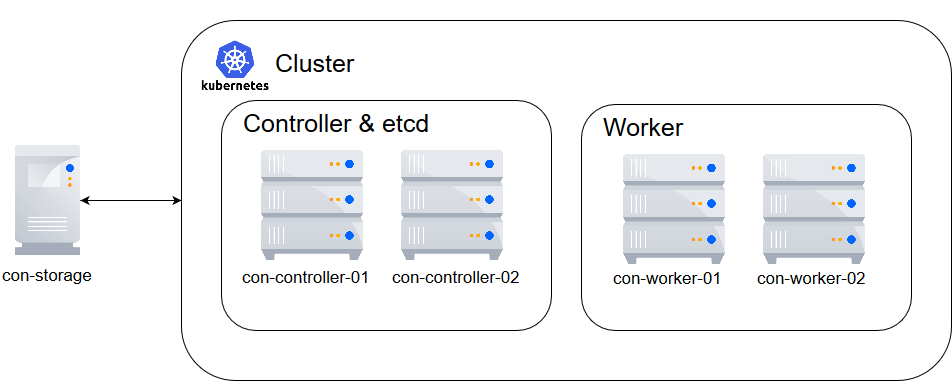
\includegraphics[width=1\textwidth,angle=0]{gfx/cluster_alt.png}
\caption[Cluster: Aktuelle Architektur]{Cluster: Aktuelle Architektur}
\label{fig:clusteralt}
\end{figure}
Um den Zustand und die Daten der Anwendungen zu speichern, wurde zuerst eine auf einem Blockspeicher basierende Speicherlösung eingesetzt, welche direkt im Kubernetes Cluster lief. Im Laufe des Projekts wurde diese, da sie kein \ac{RWX} unterstützt, durch einen zentralen NFS Server ersetzt. Diese virtuelle Maschine ist nicht redundant ausgelegt, befindet sich aber innerhalb einer Backup-Routine, welche täglich eine Sicherung des Systems erstellt. Die Datenträger für die Pods werden dynamisch durch den \textit{nfs-client-provisioner} (siehe \ref{eva:nfskube}) erzeugt, wobei die Konfiguration dieser über die Parameter der Helm Charts erfolgt.

\section{Planung}
\label{sec:planung}
Während der Planung der Integration von GlusterFS in das Kubernetes Cluster stellt sich zunächst die zentrale Frage, ob die Persistenzlösung innerhalb des Kubernetes Clusters oder als eigenständiges Speichercluster agieren soll. Während die Integration innerhalb des Kubernetes Clusters Vorteile wie eine schnelle Installation und eine gute Skalierbarkeit mit sich bringt, hilft das Aufsetzen außerhalb des Clusters dabei eine bessere Trennung zu schaffen. Da sich das Projekt im ständigen Wandel befindet und dies ebenfalls das Kubernetes Cluster betrifft, soll das GlusterFS-Cluster möglichst unabhängig agieren. Für die Installation stehen mehrere Hilfsmittel bereit. Neben der offiziellen Dokumentation bietet Gluster auch Skripte für die automatische Installation über Ansible, einem Tool für das automatische Aufsetzen und Konfigurieren von Systemen. \medskip

Durch das Aufbauen eines Speicherclusters verändert sich die Architektur des Clusters. Dabei wird der vorher für die Speicherung zuständige zentrale NFS-Server durch ein GlusterFS Cluster ersetzt. Für dieses werden drei virtuelle Maschinen erstellt, welche im Verbund für die Speicherung zuständig sind. Durch das Verwenden von drei Servern ist es möglich, durch eine dreifache Redundanz die Chance auf einen Split-Brain Zustand gering zu halten.
%evtl 3 Replicas wegen Split brain
\begin{figure}[htb]
\centering
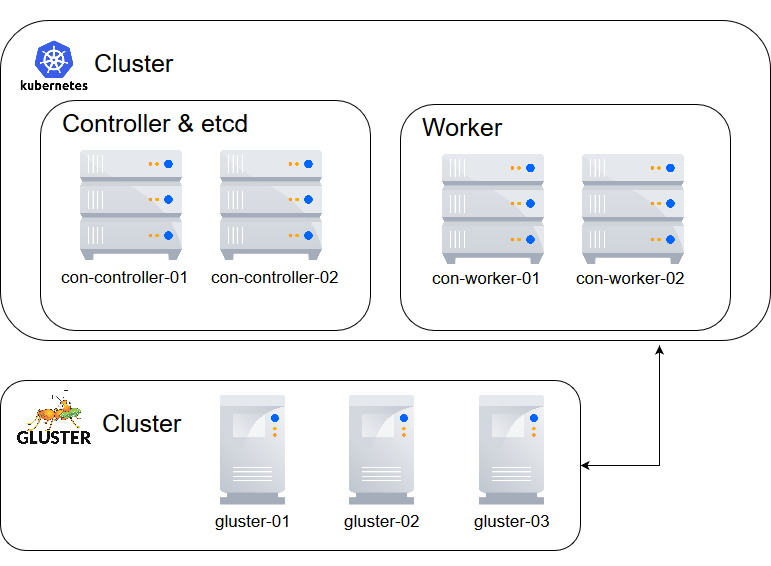
\includegraphics[width=1\textwidth,angle=0]{gfx/cluster_neu.png}
\caption[Cluster: Neue Architektur]{Cluster: Neue Architektur}
\label{fig:clusterneu}
\end{figure}
Die Abbildung \ref{fig:clusterneu} zeigt den geplanten zukünftigen Aufbau des Systems. Während am Kubernetes Cluster keine Änderung durchgeführt wurde, wurde der NFS Server durch ein Speichercluster aus drei Systemen ersetzt. Dieses agiert als eigenes Cluster und kann so auch unabhängig vom Kubernetes Cluster betrieben und auch in anderen Projekten verwendet werden. 


\section{Umsetzung}
Die Integration von GlusterFS in das Kubernetes Cluster besteht aus zwei Schritten. Sie beginnt mit dem Aufsetzen der virtuellen Maschinen und der Installation und Konfiguration des Speicherclusters. Sobald dieses eigenständige System funktional ist, beginnt mit der Integration in das Kubernetes Cluster und dem Einrichten für die dynamische Datenträgererstellung der zweite Schritt.

\subsection{Installation und Konfiguration von GlusterFS}
Die Umsetzung beginnt mit dem Erzeugen drei neuer virtueller Maschinen. Diese erhalten jeweils ein Gigabyte Arbeitsspeicher, zwei Prozessorkerne sowie zwei Festplatten. Die Erste ist dabei für die Linux-Distribution Debian und die Daten des Betriebssystems zuständig während auf der Zweiten die Daten von GlusterFS abgelegt werden.
Um die Installation und Konfiguration möglichst einfach zu halten, wird dies aus einer Kombination von mehreren Skripten für Ansible umgesetzt. Für die Installation unter Debian wird die von Jeff Geerling auf Github veröffentlichte Rolle für Ansible genutzt \cite{gluster:ansibledebian}. \medskip

Ist die Installation abgeschlossen, wird die Konfiguration über die von Gluster veröffentlichten Ansible Rollen \cite{gluster:ansible} vorgenommen. Diese enthalten unterschiedliche Rollen für Wartung, die Aktivierung von Funktionen, das Aufsetzen und Verwalten des Clusters und das Erstellen und Verwalten von Datenträgern.
Für die Konfiguration müssen unter Nutzung der Rolle \textit{gluster.infra} zuerst die Datenträger erstellt und anschließend diese und das Speichercluster durch \textit{gluster.cluster} konfiguriert werden. Werden hier bereits virtuelle Datenträger für die Verwendung im Kubernetes Cluster oder in einem anderen Projekt erstellt, bieten die Parameter die Möglichkeit, die Anzahl an Redundanzen und weitere Einstellungen zu konfigurieren. \medskip

Abschließend werden die neuen Systeme noch in eine Backup-Routine integriert. Dafür wird das Skript, welches bereits beim zentralen NFS Server genutzt wurde, erneut verwendet. 


\subsection{Einbinden von GlusterFS in Kubernetes}
Nachdem das Speichercluster installiert wurde, kann es im Kubernetes Cluster für die dynamische Erstellung von Datenträgern eingerichtet werden. Eine Möglichkeit wäre das Einbinden eines zuvor erstellten virtuellen Datenträgers durch den bereits verwendeten \textit{nfs-client-provisioner}. Dies würde bedeuten, dass alle gespeicherten Daten in getrennten Verzeichnissen auf diesem Datenträger erzeugt werden. \medskip


Um für jede Anwendung automatisch einen virtuellen Datenträger in GlusterFS erstellen zu lassen, welcher an die Nutzer der Anwendung ausgehändigt werden kann, wird Heketi benötigt. Heketi ist eine Software, welche eine \ac{REST} Schnittstelle für das Erzeugen und Verwalten von GlusterFS-Datenträgern bietet. \medskip

Um diese Anwendung zu installieren, sind einige Schritte notwendig \cite{gluster:includekubernetesteps}. Um diese Schritte zu automatisieren, hat Gluster ein Skript veröffentlicht \cite{gluster:includekubernete}. Durch dieses wird Heketi im Kubernetes Cluster bereitgestellt und die Kommunikation mit dem Speichercluster sichergestellt. Damit Heketi einwandfrei funktioniert, wird noch eine passende \textit{topology.json} benötigt. In dieser Datei werden, damit Heketi die Architektur des Speicherclusters kennt, die einzelnen Nodes des GlusterFS Systems, sowie ihr Hostname, ihre IP-Adresse und ihre Datenträger definiert.

\section{Fazit}
Der Wechsel von einem zentralen NFS Server als Speicherlösung auf ein GlusterFS Cluster war durch die verfügbaren Skripte einfach möglich. Auch bieten diese Skripte Funktionen für die Verwaltung und Wartung des Clusters wie zum Beispiel die Skalierung und das manuelle Erstellen von Datenträgern. \medskip

Die Verwendung im Kubernetes Cluster gestaltet sich durch die Verwendung von Heketi ebenfalls einfach. Wie auch zuvor bei dem NFS Server ist es nach der Integration im Kubernetes Cluster möglich, ohne die unterliegende Architektur des Speichers zu bemerken, Datenträger dynamisch erstellen zu lassen. Diese können anschließend bei Bedarf durch Dritte eingebunden und modifiziert werden.
% MEHR MEHR MEHR - Eigene Erfahrungen
\chapter{Zusammenfassung und Ausblick}
\label{cha:schluss}
Dieses Kapitel bildet den Abschluss dieser Thesis und dient dazu, die Ergebnisse zusammenzufassen und einen Ausblick auf zukünftige Themen zu bieten.

\section{Zusammenfassung} % (fold)
\label{sec:zusammenfassung}
Diese Bachelorarbeit beschäftigte sich mit dem Finden einer geeigneten Kubernetes Persistenzlösung für das aktuelle Projekt, die prototypische Umsetzung der ALM v2. Dabei wurde zuerst die Idee des Projektes betrachtet und mögliche Anwendungsfälle der Software analysiert und basierend darauf Anforderungen erstellt, welche für die Evaluation der Speicherlösungen verwendet wurden. \medskip

Anschließend wurden die in der Kubernetes Dokumentation genannten Volume Plugins mit den funktionalen Anforderungen, wie den Zugriffsmodi oder die On-Premises Kompatibilität, abgeglichen, um die zu evaluierenden Speicherlösungen einzugrenzen. Dabei zeigte sich, dass fünf Lösungen diese Anforderungen erfüllen und für die weitere Analyse und Bewertung infrage kommen. \medskip

Anforderungen wie die Datensicherheit erfüllten nahezu alle Persistenzlösungen. Die größten Unterschiede zeigten sich im Ressourcenbedarf. Während NFS die wenigsten Ressourcen benötigt, muss um alle Anforderungen zu erfüllen auf verschiedene zusätzliche Software zurückgegriffen werden, was sowohl die Komplexität erhöht als auch die Wartbarkeit verschlechtert. Daher fiel die Entscheidung auf GlusterFS, welche bis auf die Datensicherung alle Anforderungen ohne zusätzliche Software erfüllt und auf virtuellen Maschinen mit einer moderaten Ausstattung lauffähig ist. Als Abschluss der Evaluation wurde eine Handlungsempfehlung formuliert. \medskip

Nach der Auswahl der geeignetsten Software wurde das bestehende System analysiert und ein Konzept für die Umsetzung der Handlungsempfehlung erarbeitet. Um die vorher existierende Lösung zu ersetzen, wurde ein eigenständiges GlusterFS Cluster erstellt, welches eigenständig lauffähig ist und nicht im Kubernetes Cluster läuft. Für diese Installation, sowie die Integration in das existierende Cluster stehen Skripte zur Verfügung, welche eine fast vollständig automatisierte Einrichtung ermöglichen. Für die Datensicherung wurde das neue System, wie auch zuvor das alte, in eine Backup-Routine integriert. \medskip

\section{Ausblick} % (fold)
\label{sec:ausblick}
In dieser Bachelorarbeit wurde ein geeignetes Konzept für die Speicherung von Daten für die prototypische ALM v2.0 entworfen. Da das Projekt im ständigen Wandel ist, ist es nötig, diese Entscheidung bei wechselnden Anforderungen erneut zu hinterfragen. \medskip

Zusätzlich ist die Entwicklung der in Kubernetes verfügbaren Persistenzlösungen zu verfolgen. Durch die CSI und Flexvolume Schnittstelle ist für Dritte möglich, neue Volume Plugins zu entwickeln, welche für die Anforderungen gut geeignet sind. Neue Lösungen wie \textit{Rook}\footnote{\label{foot:rook}https://github.com/rook/rook}, welches sich zurzeit in der Entwicklung befindet und in noch keiner stabilen Version vorliegt, vereinen mehrere Anwendungen wie zum Beispiel Ceph, NFS und den verteilten Object Speicher Minio in einer Lösung. Sie bieten daher die Möglichkeit, für unterschiedliche Einsatzzwecke universal genutzt zu werden. \medskip

Als letzter Punkt sind die möglichen Einsatzzwecke, um welche das GlusterFS System erweitert werden kann, zu betrachten. So können die derzeit noch im Unternehmen verwendenden NFS Servern in der Speicherlösung integriert werden oder ein Standortübergreifendes Speichersystem aufgebaut werden.
% Cloudtechnologien
% Messungen mehr
% Backups auf Glusterfs sinnvoll?
% evtl für it? falls es sich bewährt
%Configsmap?

%kubectl erklären
%RWX für cluster atlassian
%Erklären, dass ROok noch in etnwicklung ist.
%\include{chapters/examples/chapter01}
%\include{chapters/examples/chapter02}
%\include{chapters/examples/chapter03}
%*************************************************************************
% Other Stuff in the Back
%*************************************************************************
\cleardoublepage%********************************************************************
% Bibliography
%*******************************************************
% work-around to have small caps also here in the headline
% https://tex.stackexchange.com/questions/188126/wrong-header-in-bibliography-classicthesis
% Thanks to Enrico Gregorio
\defbibheading{bibintoc}[\bibname]{%
  \phantomsection
  \manualmark
  \markboth{\spacedlowsmallcaps{#1}}{\spacedlowsmallcaps{#1}}%
  \addtocontents{toc}{\protect\vspace{\beforebibskip}}%
  \addcontentsline{toc}{chapter}{\tocEntry{#1}}%
  \chapter*{#1}%
}
{\raggedright
\printbibliography[heading=bibintoc]
}

%*************************************************************************
% Backmatter
%*************************************************************************
\appendix
%\renewcommand{\thechapter}{\alph{chapter}}
\cleardoublepage
\part{Appendix}
%********************************************************************
% Appendix
%*******************************************************
% If problems with the headers: get headings in appendix etc. right
%\markboth{\spacedlowsmallcaps{Appendix}}{\spacedlowsmallcaps{Appendix}}
\chapter{Anhang}
\section{Kubernetes Persistenzlösungen}
\begin{table}[h!]
    \centering
    \begin{tabular}{lcccc} \hline
    \textbf{Volume Plugin} & \textbf{On-Premises} & \textbf{RWO} & \textbf{ROX} & \textbf{RWX}\\ \hline
    AWSElasticBlockStore & & x & & \\
    AzureFile & & x & x & x \\
    AzureDisk & & x & & \\
    CephFS & x & x & x & x\\
    CSI & \multicolumn{4}{c}{Abhängig von Treiber} \\
    Cinder & x & x & & \\
    emptyDir & x & x& & \\
    FC & x & x & x & \\
    Flexvolume & \multicolumn{4}{c}{Abhängig von Treiber} \\
    Flocker & x & x & & \\
    GCEPersistentDisk & & x & x& \\
    Glusterfs & x & x & x& x\\
    HostPath & x & x & & \\
    iSCSI & x & x &x & \\
    %local & x & x& &\\
    Quobyte & x & x & x& x\\
    NFS & x & x & x& x\\
    RBD & x & x &x & \\
    VsphereVolume & x & x & & \\
    PortworxVolume & x & x & & x \\
    ScaleIO & x & x & x& \\
    StorageOS & x & x & & \\

	 \end{tabular}
    \caption{Volume Plugins in der Kubernetes Dokumentation}
    \label{marktuebersicht}
 \end{table}
%\include{chapters/examples/appendix01}
%\include{chapters/examples/appendix02}

%*************************************************************************
% Game Over: Restore, Restart, or Quit?
%*************************************************************************
\end{document}
%*************************************************************************
